\subsection{Erweiterte Utility-Spike-Maps nach Scope und Gewichtungsprofil}
\label{app:utility-spike-erweitert}

Die folgenden Abbildungen zeigen die additive Utility als dreidimensionale H/k-Landschaft. Für jedes Gewichtungsprofil werden eine transparente und eine kräftigere Variante der Utility-Ebene ausgegeben; das Treatment mit der höchsten Utility ist jeweils hervorgehoben.

\begin{longtable}{llllrrrr}
\caption{Utility-Spike-Maps: bestes Treatment je Scope und Gewichtungsprofil} \label{tab:spike-utility-best-by-scope-persona} \\
\toprule
scope & persona & figure & best\_hk & best\_utility & success\_rate\_pct & avg\_tokens\_k & avg\_runtime\_s \\
\midrule
\endfirsthead
\caption[]{Utility-Spike-Maps: bestes Treatment je Scope und Gewichtungsprofil} \\
\toprule
scope & persona & figure & best\_hk & best\_utility & success\_rate\_pct & avg\_tokens\_k & avg\_runtime\_s \\
\midrule
\endhead
\midrule
\multicolumn{8}{r}{Continued on next page} \\
\midrule
\endfoot
\bottomrule
\endlastfoot
Global & Accuracy First & fig\_08\_spike\_global\_accuracy\_first.png & h5/k5 & 0,1899 & 31,4 & 876,8 & 317,8 \\
Global & Cost Sensitive & fig\_08\_spike\_global\_cost\_sensitive.png & h10/k0 & 0,0704 & 9,0 & 120,8 & 63,2 \\
Global & Time Sensitive & fig\_08\_spike\_global\_time\_sensitive.png & h0/k5 & 0,0770 & 29,0 & 774,7 & 279,7 \\
Global & Stress 80 & fig\_08\_spike\_global\_stress\_80.png & h10/k0 & 0,0654 & 9,0 & 120,8 & 63,2 \\
GitLab & Accuracy First & fig\_08\_spike\_gitlab\_accuracy\_first.png & h5/k5 & 0,1661 & 28,1 & 967,3 & 255,0 \\
GitLab & Cost Sensitive & fig\_08\_spike\_gitlab\_cost\_sensitive.png & h5/k0 & 0,0972 & 15,8 & 251,4 & 79,4 \\
GitLab & Time Sensitive & fig\_08\_spike\_gitlab\_time\_sensitive.png & h5/k0 & 0,0974 & 15,8 & 251,4 & 79,4 \\
GitLab & Stress 80 & fig\_08\_spike\_gitlab\_stress\_80.png & h5/k0 & 0,0821 & 15,8 & 251,4 & 79,4 \\
Reddit & Accuracy First & fig\_08\_spike\_reddit\_accuracy\_first.png & h5/k5 & 0,5586 & 69,0 & 573,3 & 175,5 \\
Reddit & Cost Sensitive & fig\_08\_spike\_reddit\_cost\_sensitive.png & h5/k5 & 0,4130 & 69,0 & 573,3 & 175,5 \\
Reddit & Time Sensitive & fig\_08\_spike\_reddit\_time\_sensitive.png & h5/k5 & 0,4406 & 69,0 & 573,3 & 175,5 \\
Reddit & Stress 80 & fig\_08\_spike\_reddit\_stress\_80.png & h5/k5 & 0,3609 & 69,0 & 573,3 & 175,5 \\
Shopping & Accuracy First & fig\_08\_spike\_shopping\_accuracy\_first.png & h0/k2 & 0,1471 & 21,4 & 440,4 & 228,5 \\
Shopping & Cost Sensitive & fig\_08\_spike\_shopping\_cost\_sensitive.png & h0/k2 & 0,0811 & 21,4 & 440,4 & 228,5 \\
Shopping & Time Sensitive & fig\_08\_spike\_shopping\_time\_sensitive.png & h0/k2 & 0,0787 & 21,4 & 440,4 & 228,5 \\
Shopping & Stress 80 & fig\_08\_spike\_shopping\_stress\_80.png & h0/k0 & 0,0536 & 7,1 & 106,4 & 66,7 \\
Shopping Admin & Accuracy First & fig\_08\_spike\_shopping\_admin\_accuracy\_first.png & h2/k2 & 0,1127 & 23,6 & 1141,0 & 494,4 \\
Shopping Admin & Cost Sensitive & fig\_08\_spike\_shopping\_admin\_cost\_sensitive.png & h10/k0 & 0,0717 & 9,1 & 151,5 & 69,6 \\
Shopping Admin & Time Sensitive & fig\_08\_spike\_shopping\_admin\_time\_sensitive.png & h10/k0 & 0,0724 & 9,1 & 151,5 & 69,6 \\
Shopping Admin & Stress 80 & fig\_08\_spike\_shopping\_admin\_stress\_80.png & h10/k0 & 0,0673 & 9,1 & 151,5 & 69,6 \\
\end{longtable}


\clearpage
\subsubsection{Global}
\begin{figure}[htbp]
    \centering
    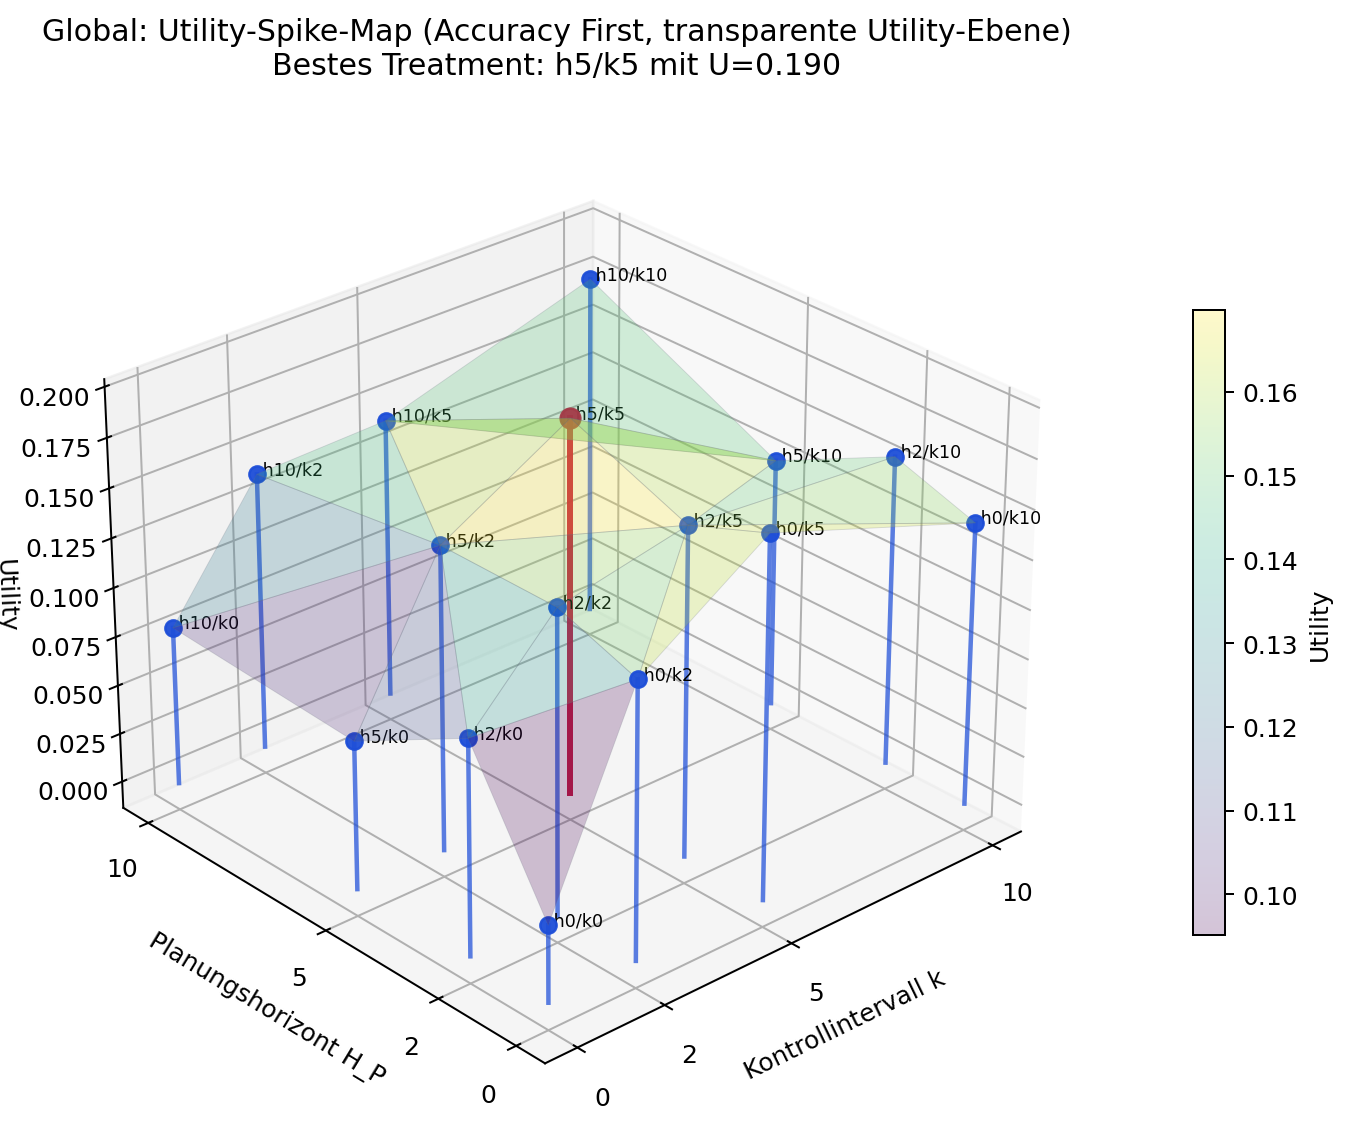
\includegraphics[width=\textwidth]
    {figures/fig_08_spike_transparent_global_accuracy_first.png}
    \caption{Global: Utility-Spike-Map mit transparenter Utility-Ebene für das Gewichtungsprofil Accuracy First}
    \label{fig:app-spike-transparent-global-accuracy-first}
\end{figure}

\begin{figure}[htbp]
    \centering
    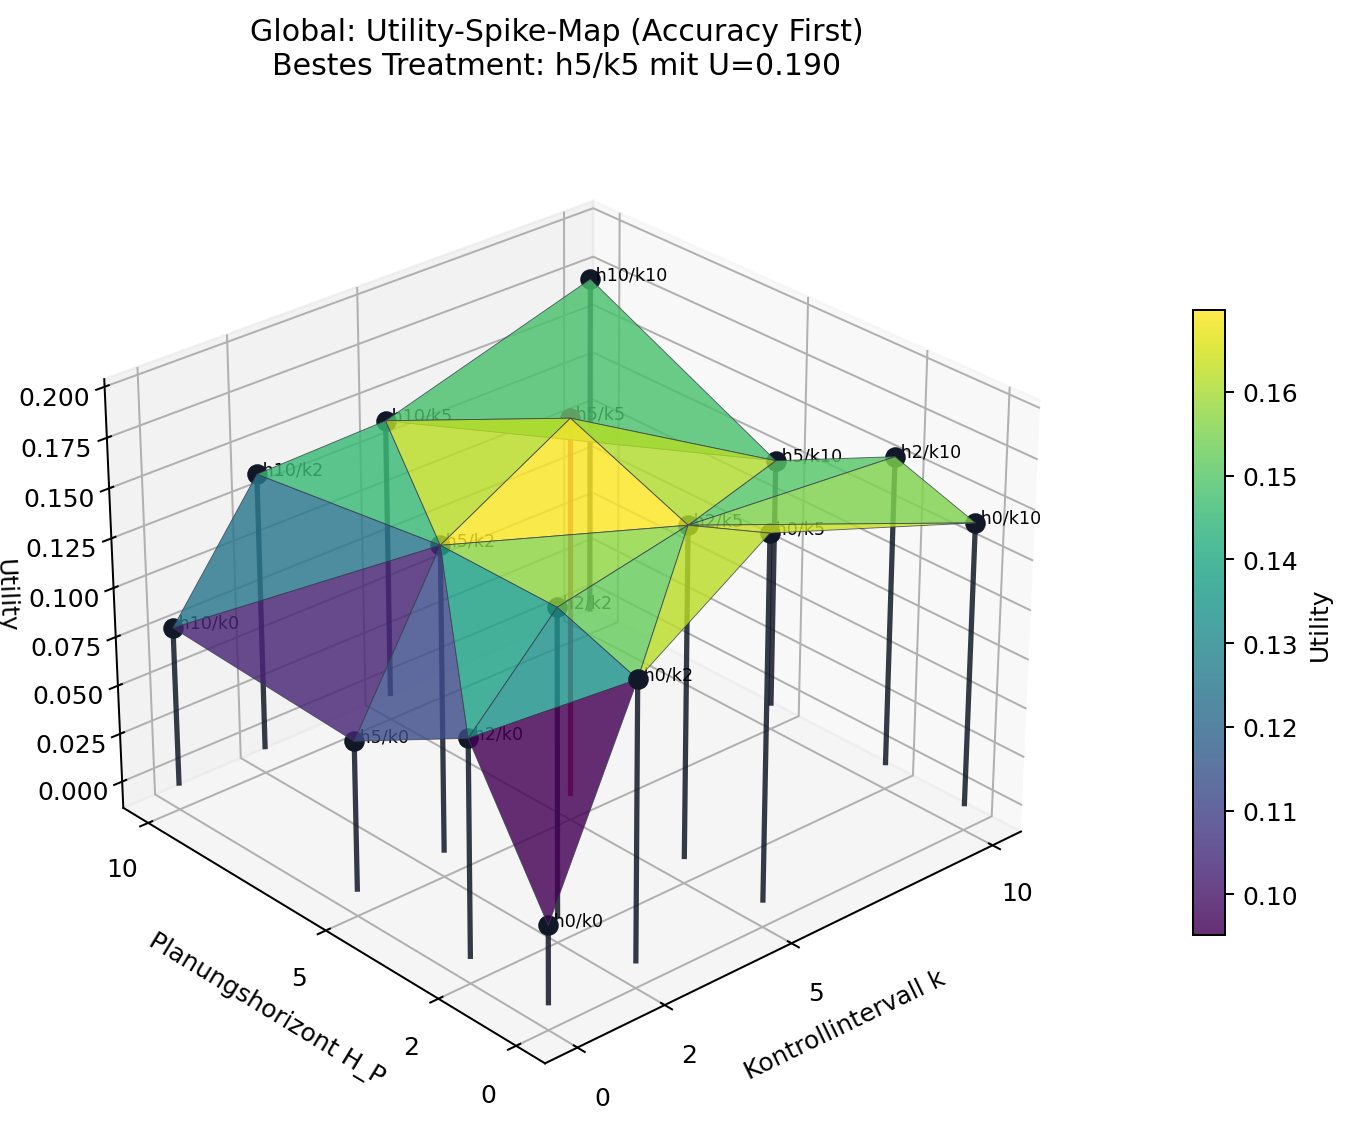
\includegraphics[width=\textwidth]
    {figures/fig_08_spike_global_accuracy_first.png}
    \caption{Global: Utility-Spike-Map mit kräftiger Utility-Ebene für das Gewichtungsprofil Accuracy First}
    \label{fig:app-spike-global-accuracy-first}
\end{figure}

\begin{figure}[htbp]
    \centering
    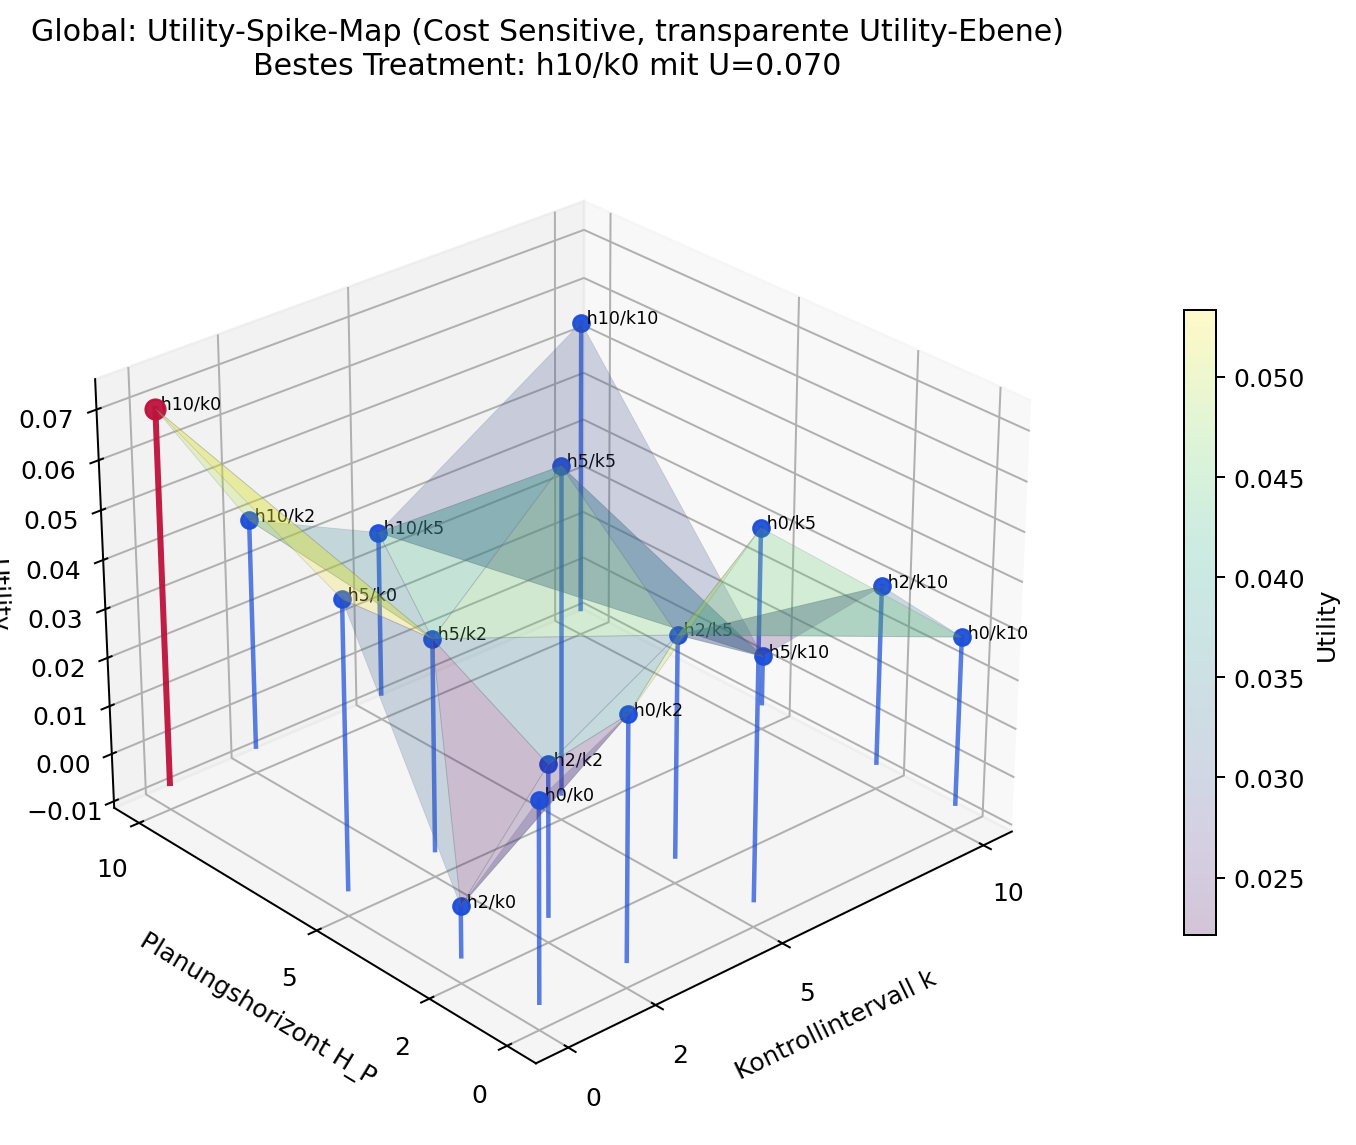
\includegraphics[width=\textwidth]
    {figures/fig_08_spike_transparent_global_cost_sensitive.png}
    \caption{Global: Utility-Spike-Map mit transparenter Utility-Ebene für das Gewichtungsprofil Cost Sensitive}
    \label{fig:app-spike-transparent-global-cost-sensitive}
\end{figure}

\begin{figure}[htbp]
    \centering
    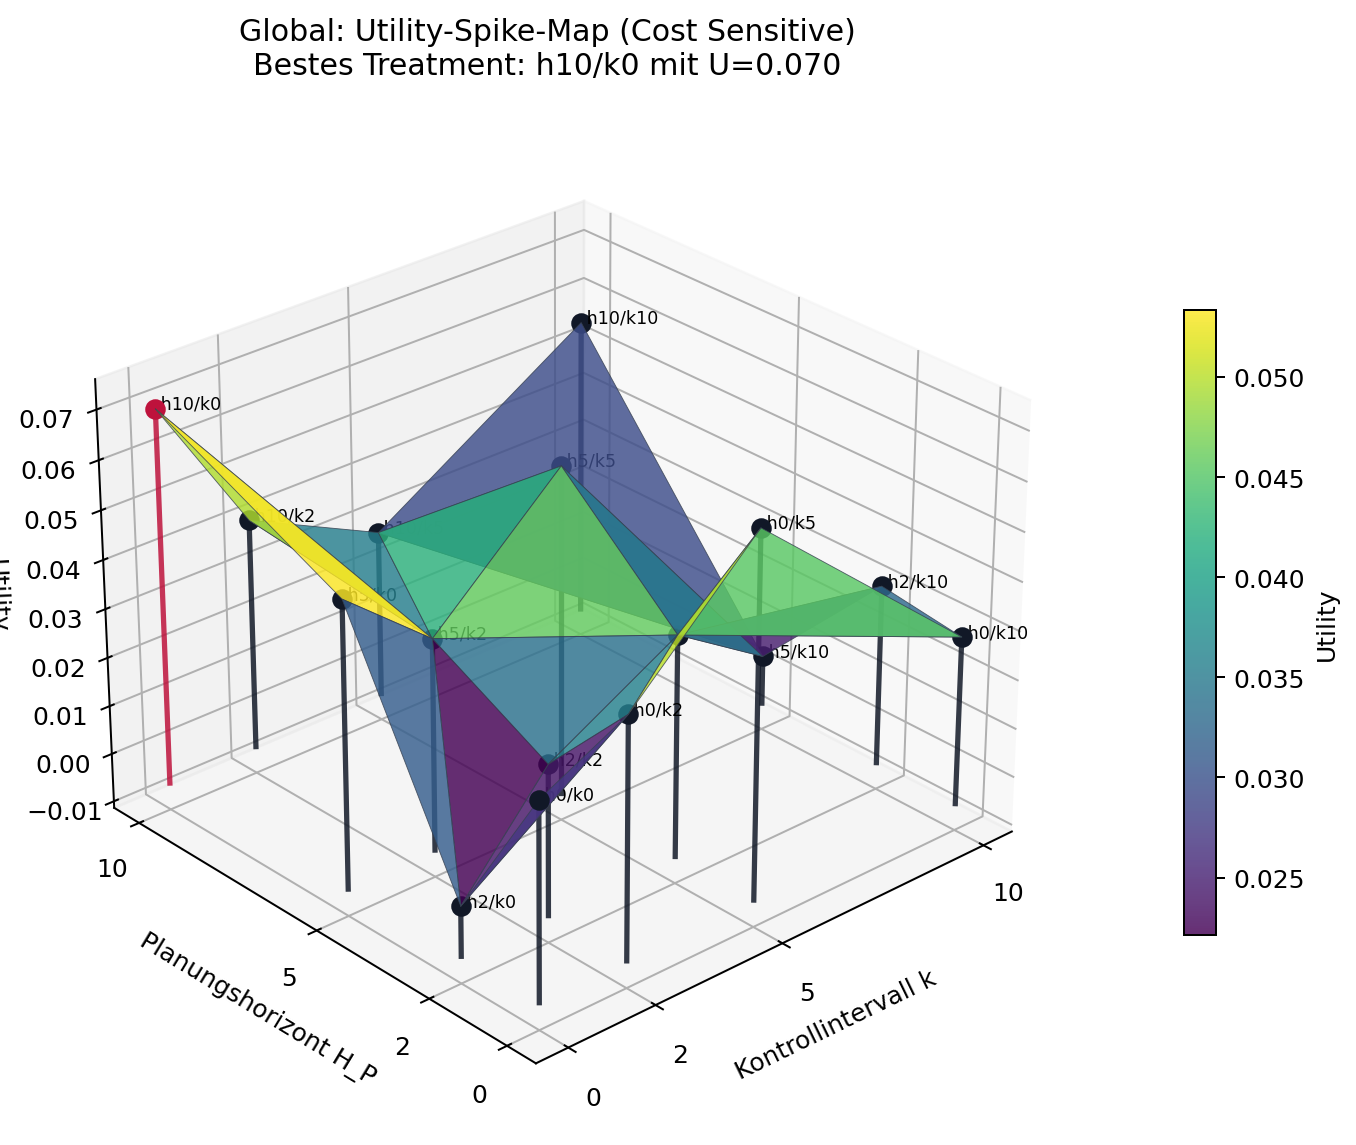
\includegraphics[width=\textwidth]
    {figures/fig_08_spike_global_cost_sensitive.png}
    \caption{Global: Utility-Spike-Map mit kräftiger Utility-Ebene für das Gewichtungsprofil Cost Sensitive}
    \label{fig:app-spike-global-cost-sensitive}
\end{figure}

\begin{figure}[htbp]
    \centering
    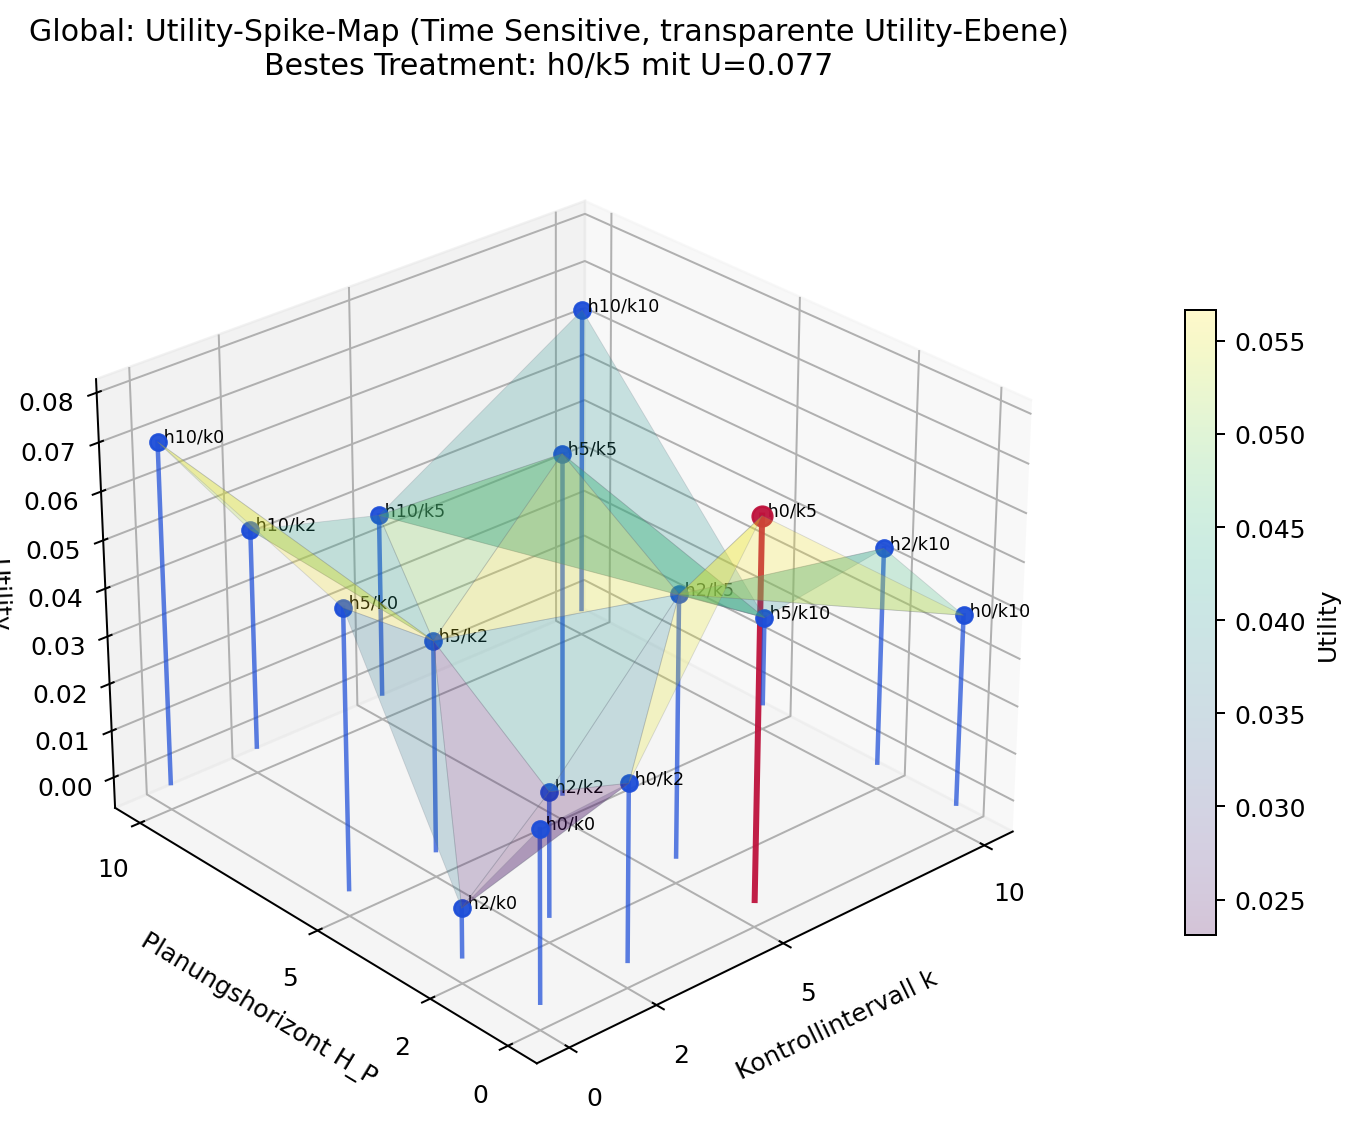
\includegraphics[width=\textwidth]
    {figures/fig_08_spike_transparent_global_time_sensitive.png}
    \caption{Global: Utility-Spike-Map mit transparenter Utility-Ebene für das Gewichtungsprofil Time Sensitive}
    \label{fig:app-spike-transparent-global-time-sensitive}
\end{figure}

\begin{figure}[htbp]
    \centering
    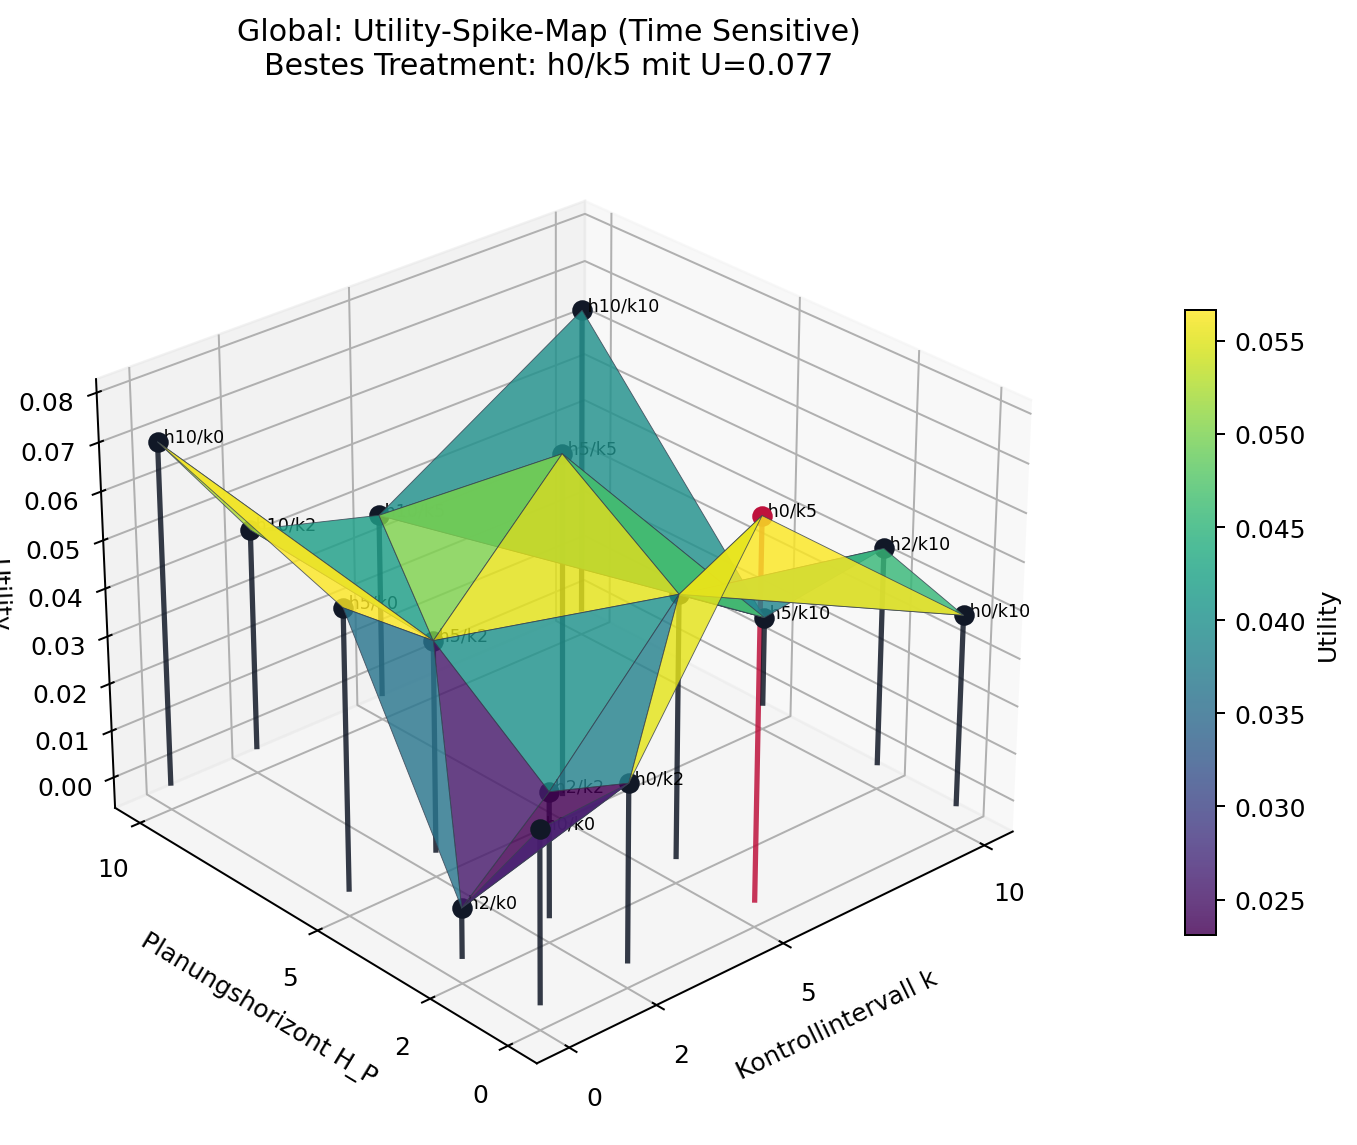
\includegraphics[width=\textwidth]
    {figures/fig_08_spike_global_time_sensitive.png}
    \caption{Global: Utility-Spike-Map mit kräftiger Utility-Ebene für das Gewichtungsprofil Time Sensitive}
    \label{fig:app-spike-global-time-sensitive}
\end{figure}

\begin{figure}[htbp]
    \centering
    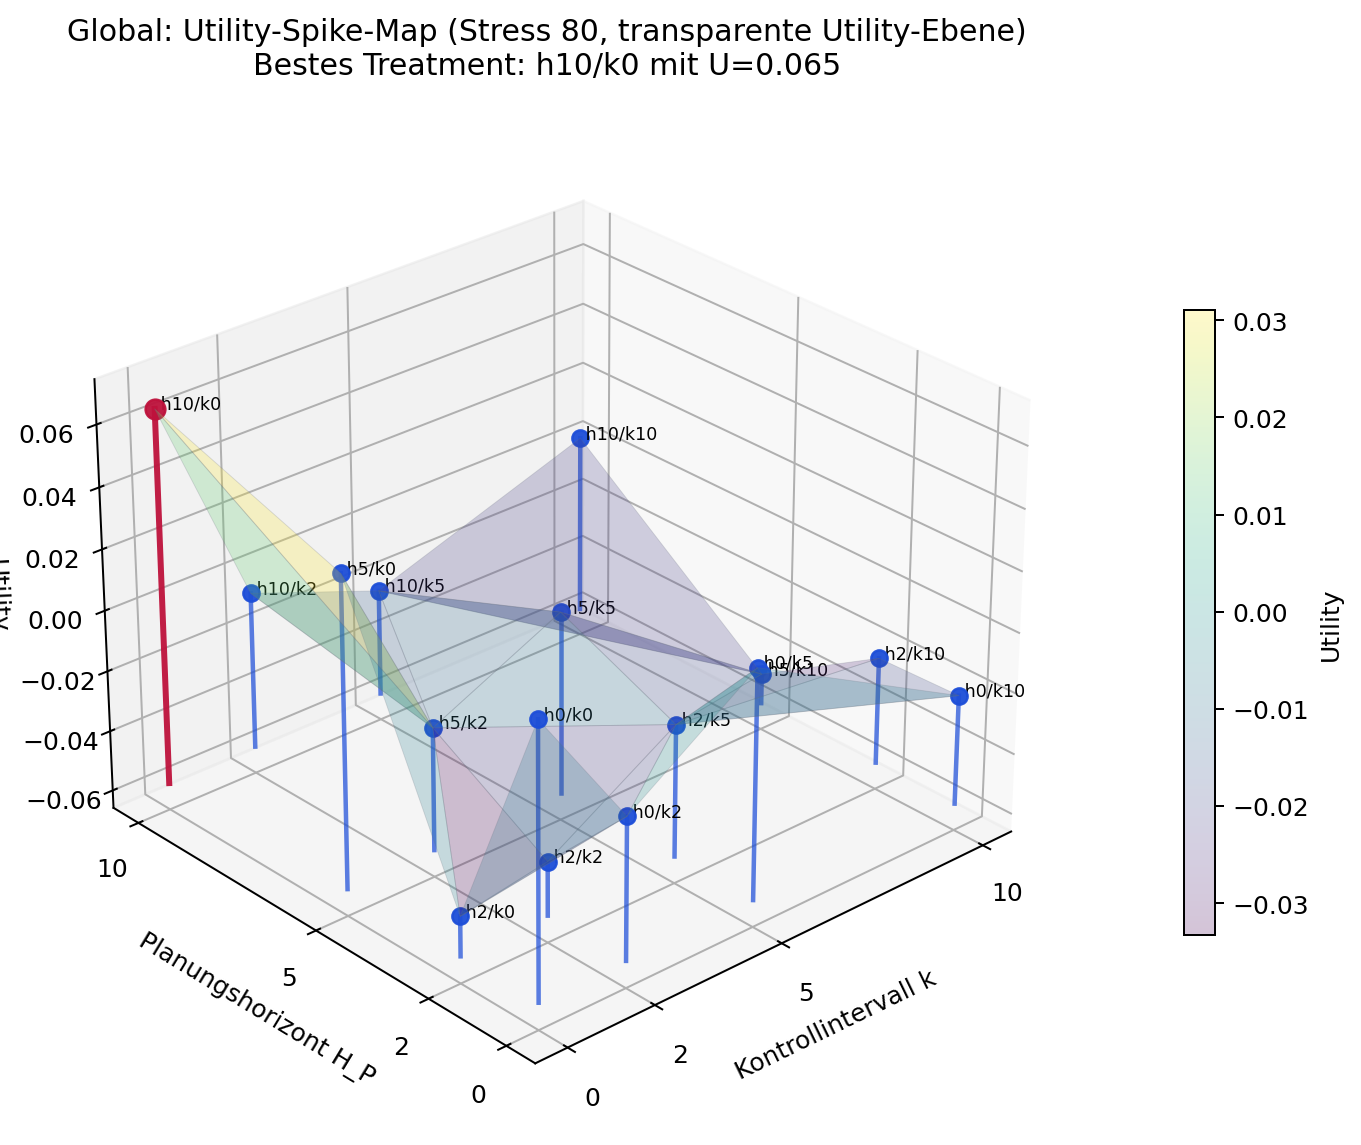
\includegraphics[width=\textwidth]
    {figures/fig_08_spike_transparent_global_stress_80.png}
    \caption{Global: Utility-Spike-Map mit transparenter Utility-Ebene für das Gewichtungsprofil Stress 80}
    \label{fig:app-spike-transparent-global-stress-80}
\end{figure}

\begin{figure}[htbp]
    \centering
    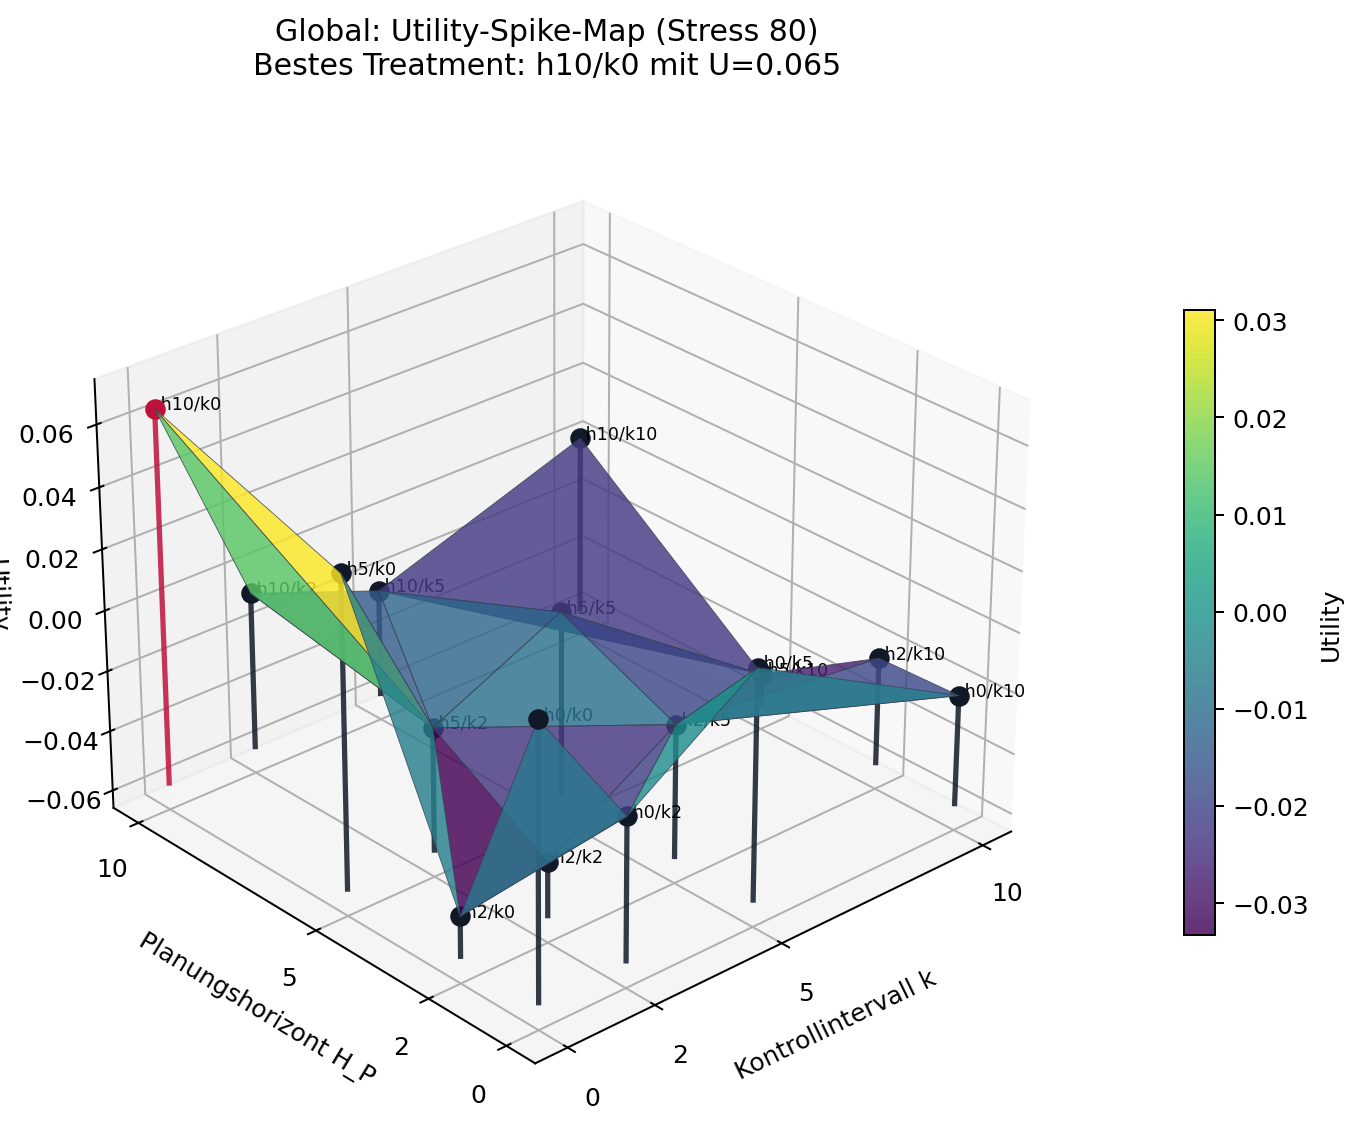
\includegraphics[width=\textwidth]
    {figures/fig_08_spike_global_stress_80.png}
    \caption{Global: Utility-Spike-Map mit kräftiger Utility-Ebene für das Gewichtungsprofil Stress 80}
    \label{fig:app-spike-global-stress-80}
\end{figure}

\clearpage
\subsubsection{GitLab}
\begin{figure}[htbp]
    \centering
    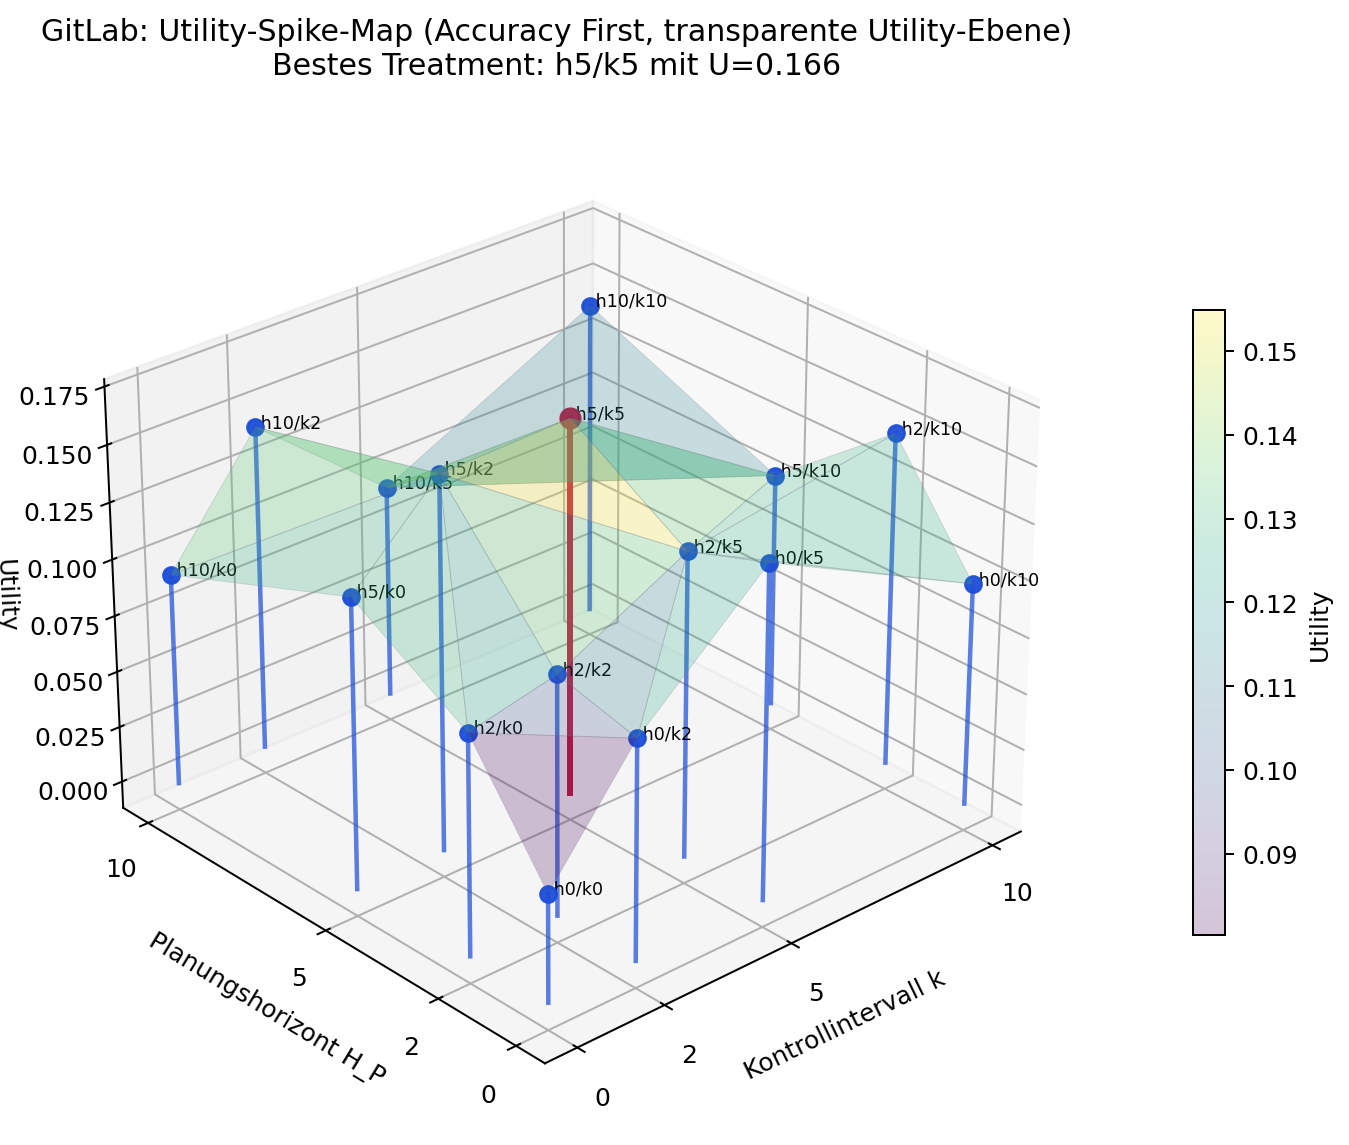
\includegraphics[width=\textwidth]
    {figures/fig_08_spike_transparent_gitlab_accuracy_first.png}
    \caption{GitLab: Utility-Spike-Map mit transparenter Utility-Ebene für das Gewichtungsprofil Accuracy First}
    \label{fig:app-spike-transparent-gitlab-accuracy-first}
\end{figure}

\begin{figure}[htbp]
    \centering
    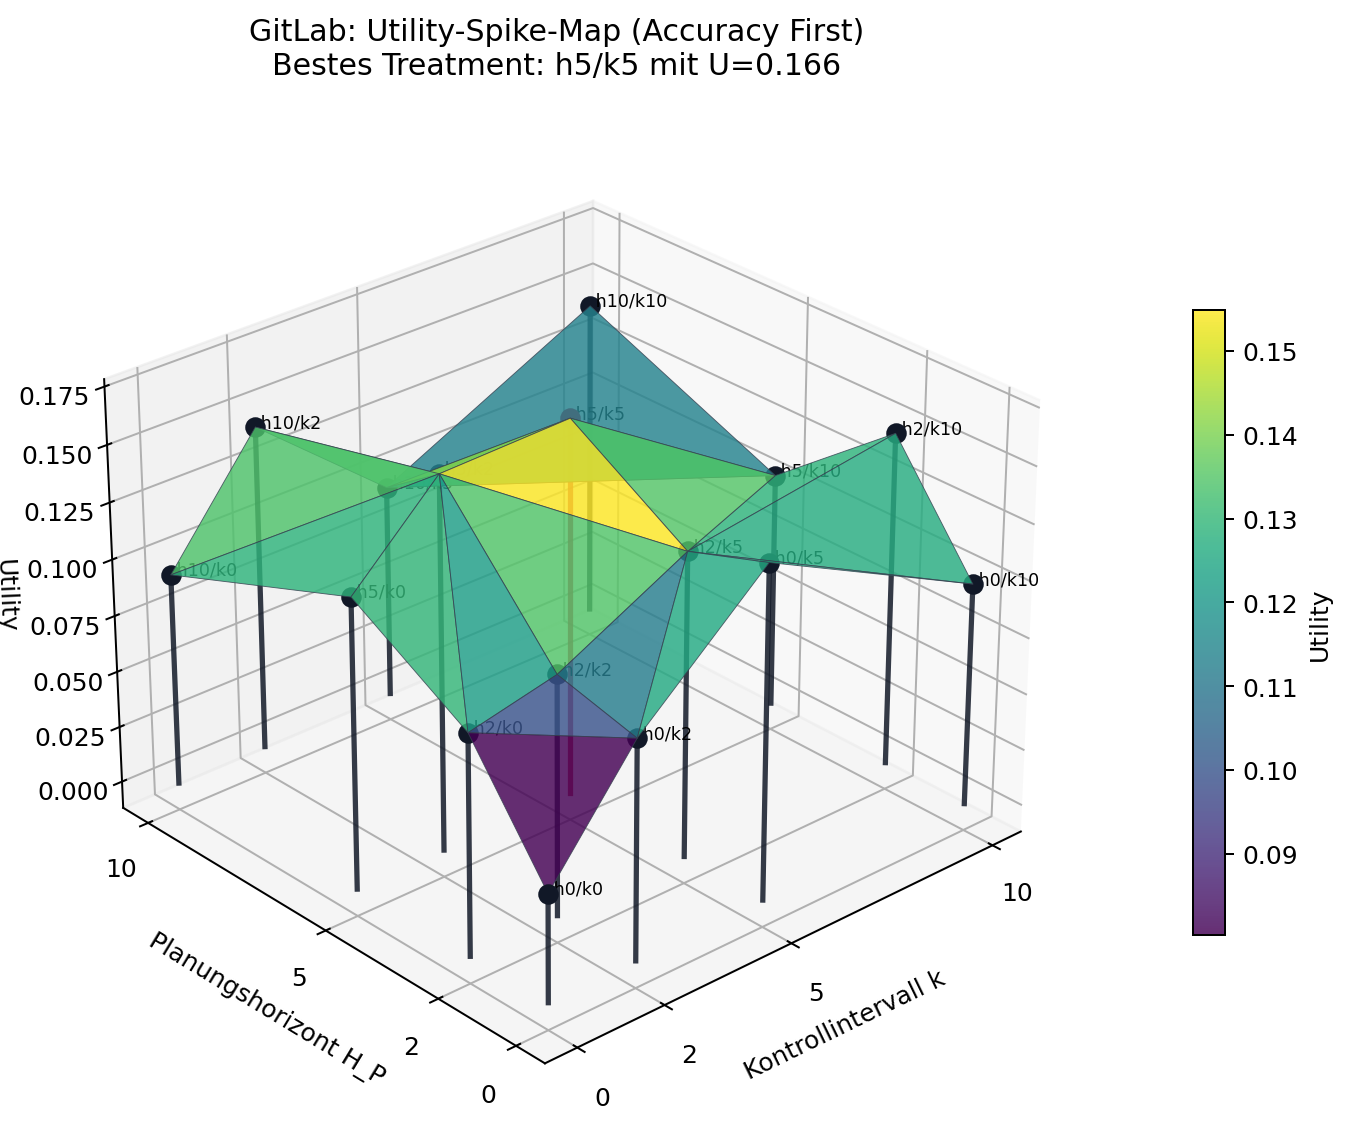
\includegraphics[width=\textwidth]
    {figures/fig_08_spike_gitlab_accuracy_first.png}
    \caption{GitLab: Utility-Spike-Map mit kräftiger Utility-Ebene für das Gewichtungsprofil Accuracy First}
    \label{fig:app-spike-gitlab-accuracy-first}
\end{figure}

\begin{figure}[htbp]
    \centering
    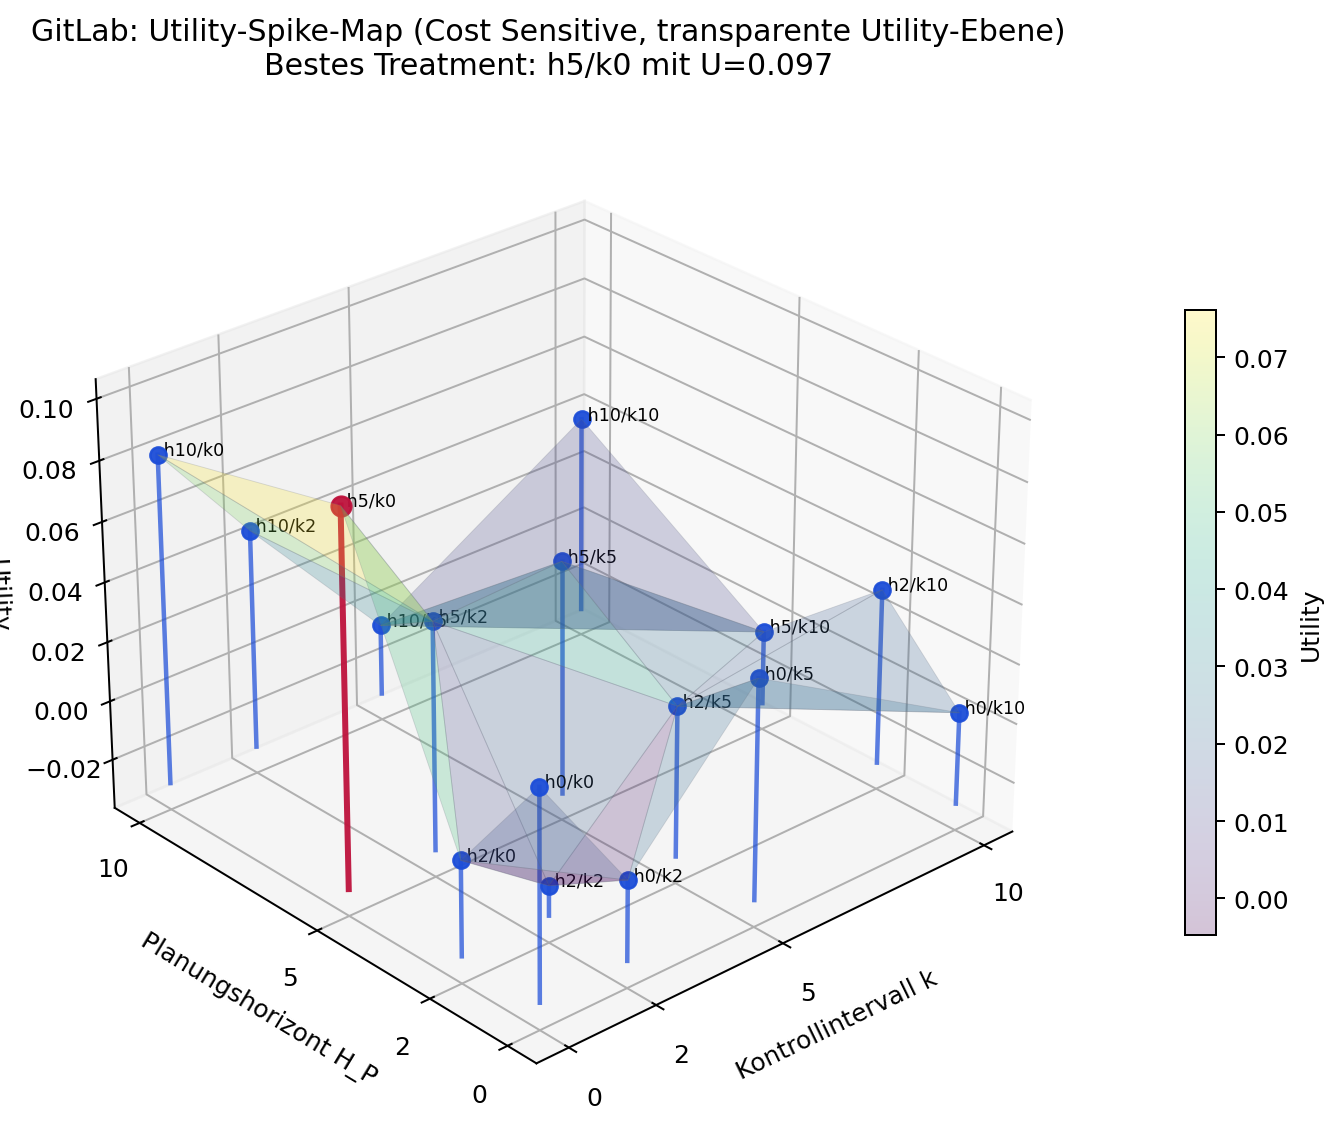
\includegraphics[width=\textwidth]
    {figures/fig_08_spike_transparent_gitlab_cost_sensitive.png}
    \caption{GitLab: Utility-Spike-Map mit transparenter Utility-Ebene für das Gewichtungsprofil Cost Sensitive}
    \label{fig:app-spike-transparent-gitlab-cost-sensitive}
\end{figure}

\begin{figure}[htbp]
    \centering
    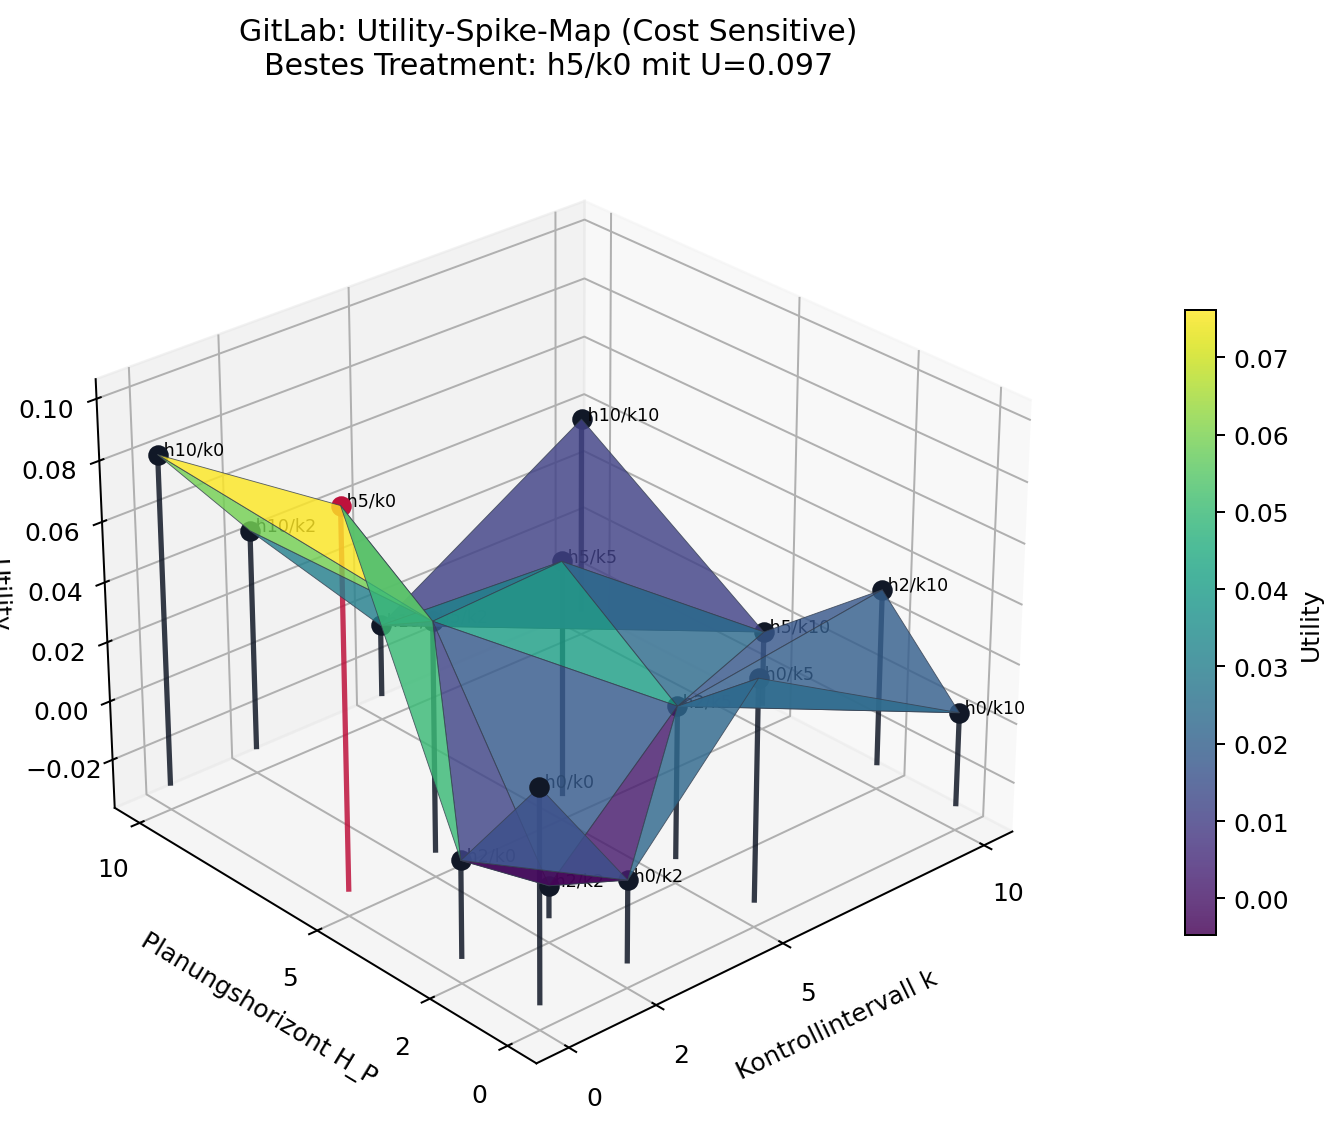
\includegraphics[width=\textwidth]
    {figures/fig_08_spike_gitlab_cost_sensitive.png}
    \caption{GitLab: Utility-Spike-Map mit kräftiger Utility-Ebene für das Gewichtungsprofil Cost Sensitive}
    \label{fig:app-spike-gitlab-cost-sensitive}
\end{figure}

\begin{figure}[htbp]
    \centering
    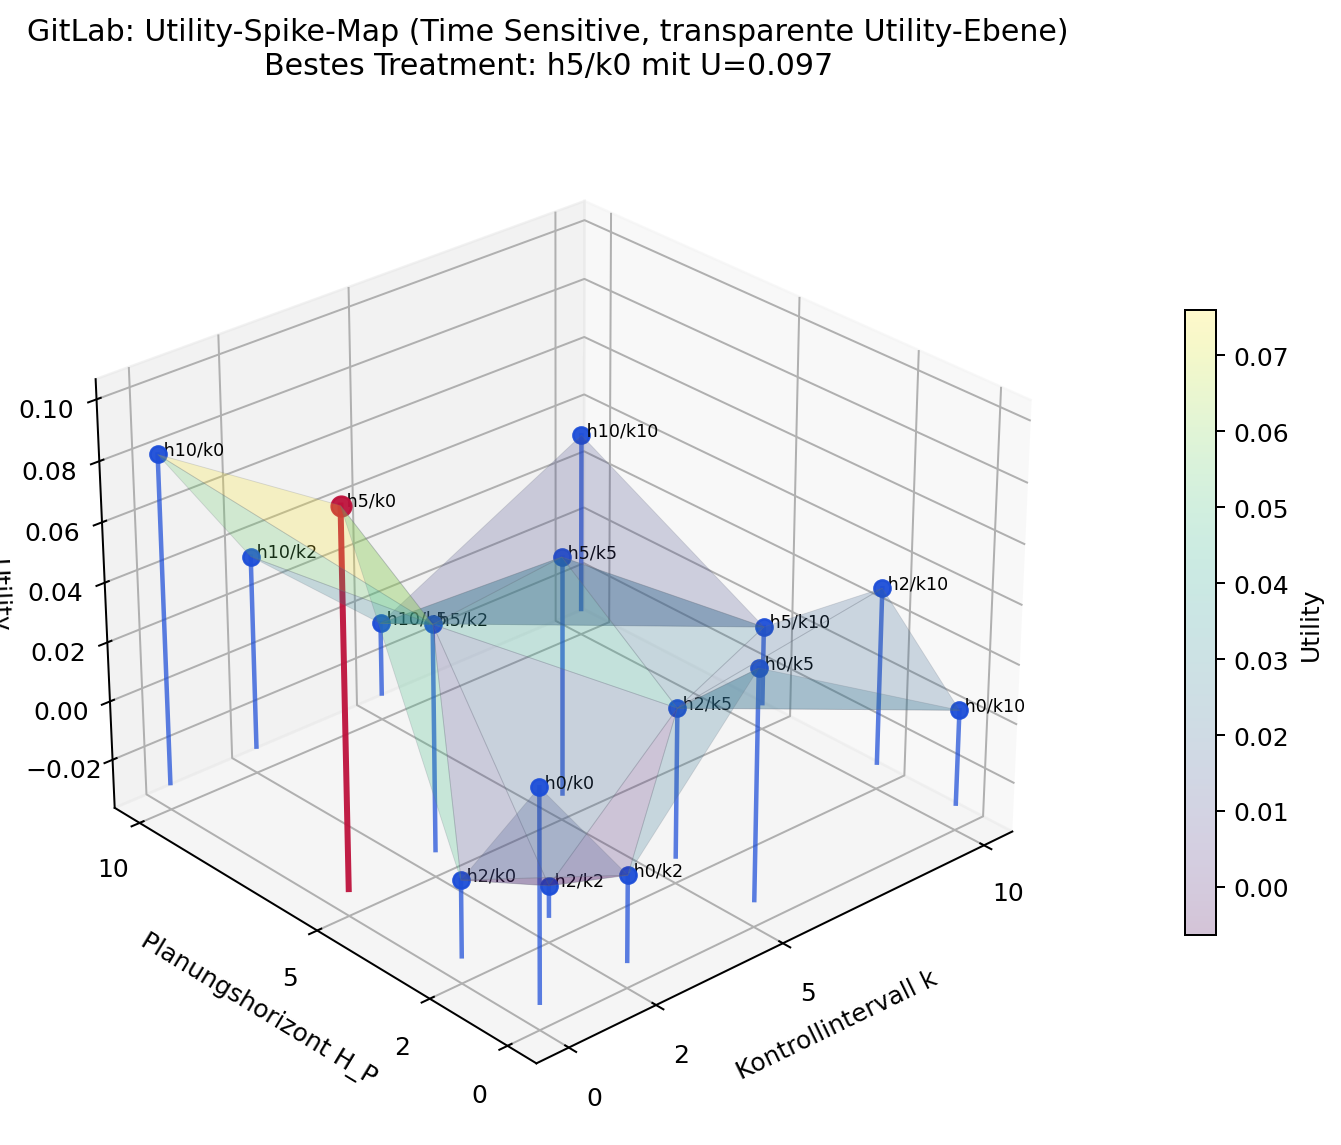
\includegraphics[width=\textwidth]
    {figures/fig_08_spike_transparent_gitlab_time_sensitive.png}
    \caption{GitLab: Utility-Spike-Map mit transparenter Utility-Ebene für das Gewichtungsprofil Time Sensitive}
    \label{fig:app-spike-transparent-gitlab-time-sensitive}
\end{figure}

\begin{figure}[htbp]
    \centering
    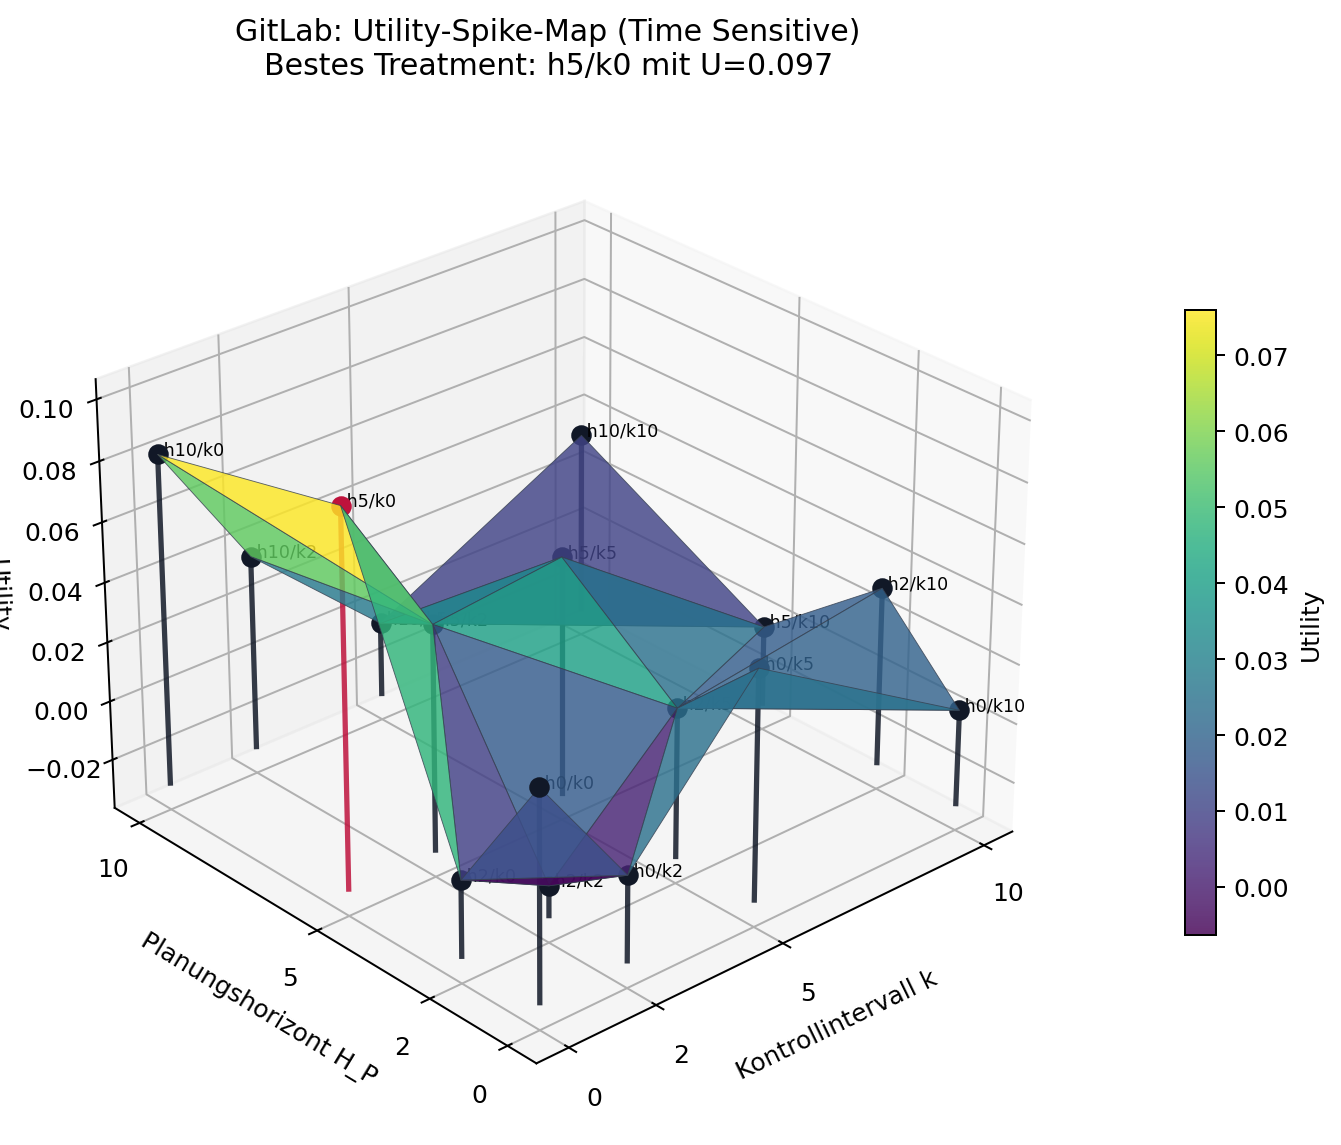
\includegraphics[width=\textwidth]
    {figures/fig_08_spike_gitlab_time_sensitive.png}
    \caption{GitLab: Utility-Spike-Map mit kräftiger Utility-Ebene für das Gewichtungsprofil Time Sensitive}
    \label{fig:app-spike-gitlab-time-sensitive}
\end{figure}

\begin{figure}[htbp]
    \centering
    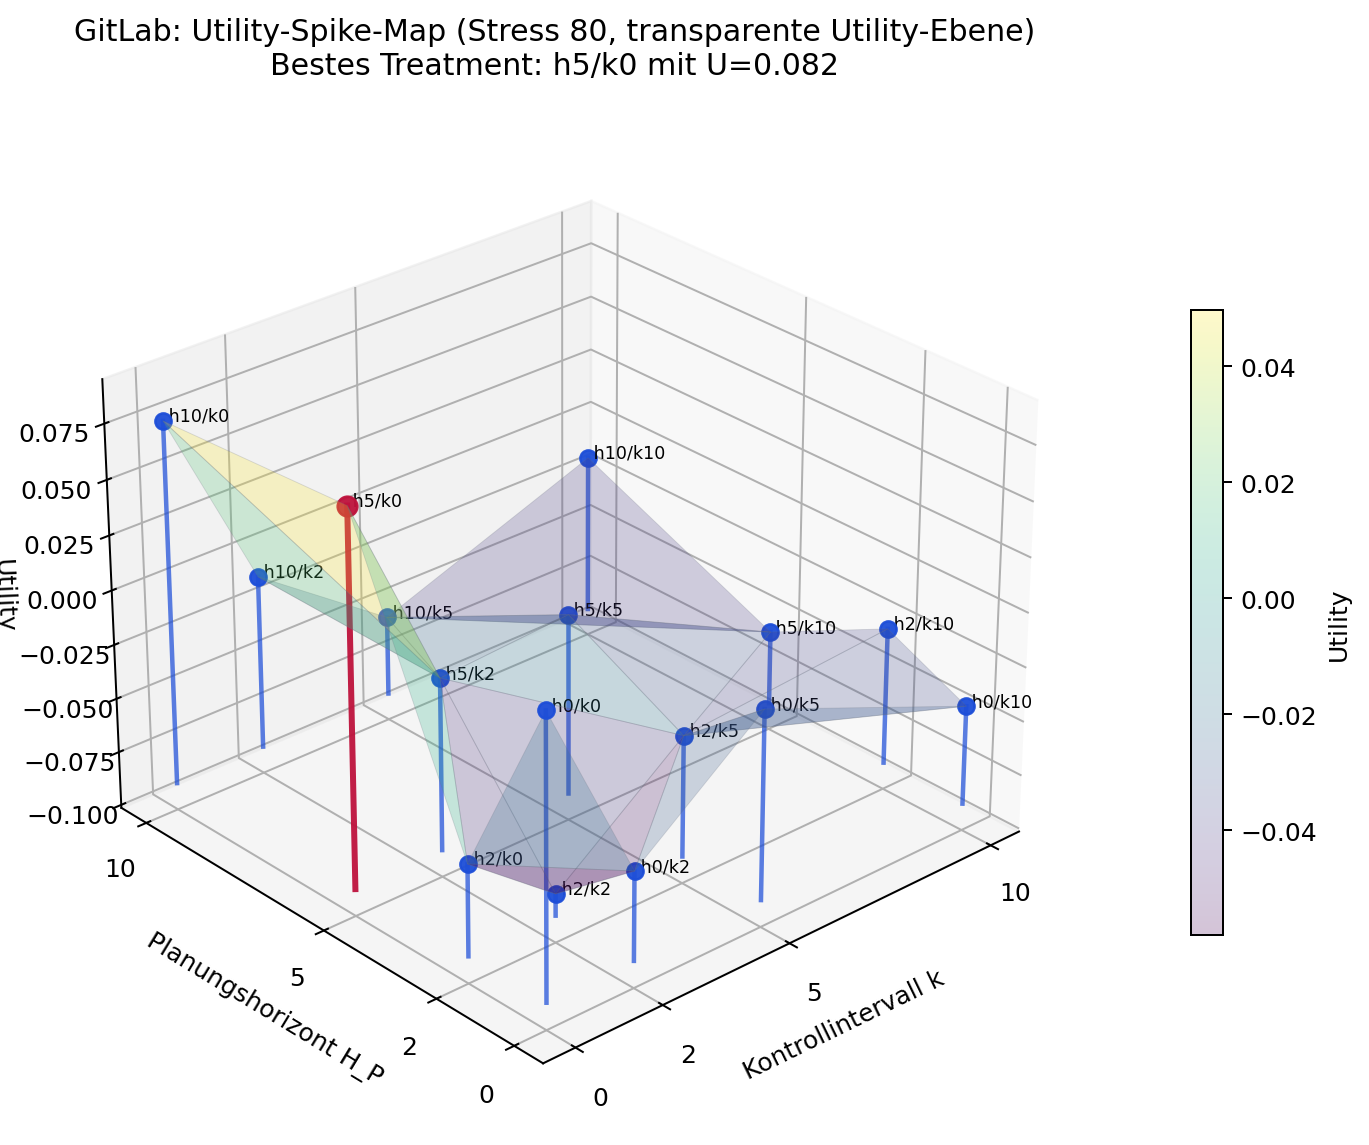
\includegraphics[width=\textwidth]
    {figures/fig_08_spike_transparent_gitlab_stress_80.png}
    \caption{GitLab: Utility-Spike-Map mit transparenter Utility-Ebene für das Gewichtungsprofil Stress 80}
    \label{fig:app-spike-transparent-gitlab-stress-80}
\end{figure}

\begin{figure}[htbp]
    \centering
    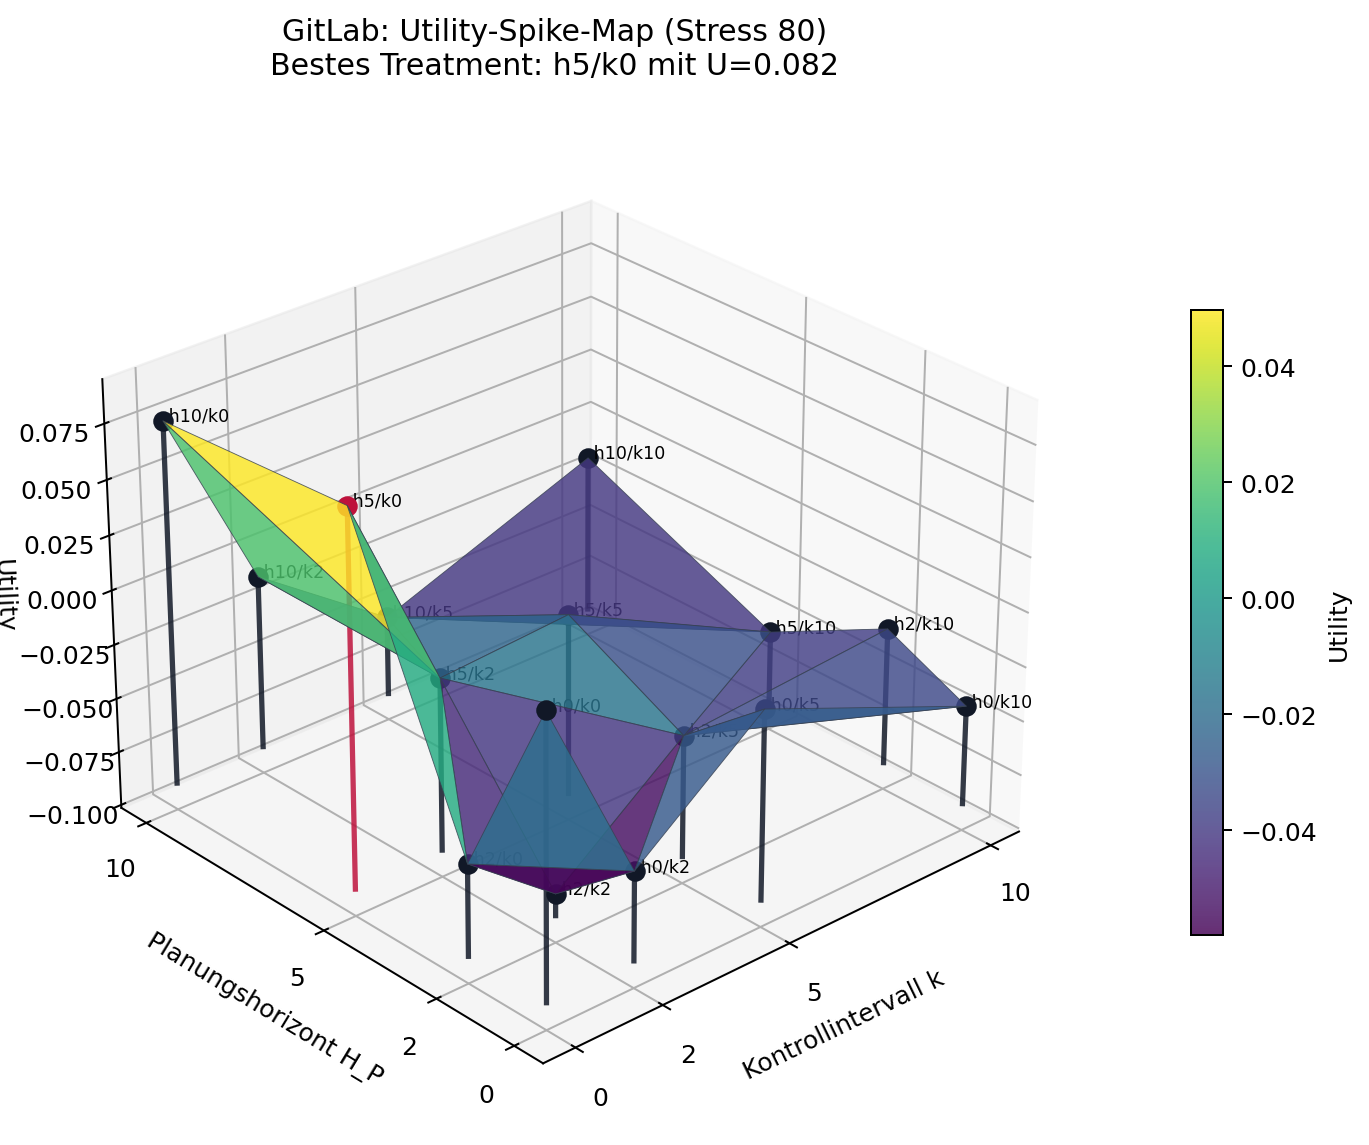
\includegraphics[width=\textwidth]
    {figures/fig_08_spike_gitlab_stress_80.png}
    \caption{GitLab: Utility-Spike-Map mit kräftiger Utility-Ebene für das Gewichtungsprofil Stress 80}
    \label{fig:app-spike-gitlab-stress-80}
\end{figure}

\clearpage
\subsubsection{Reddit}
\begin{figure}[htbp]
    \centering
    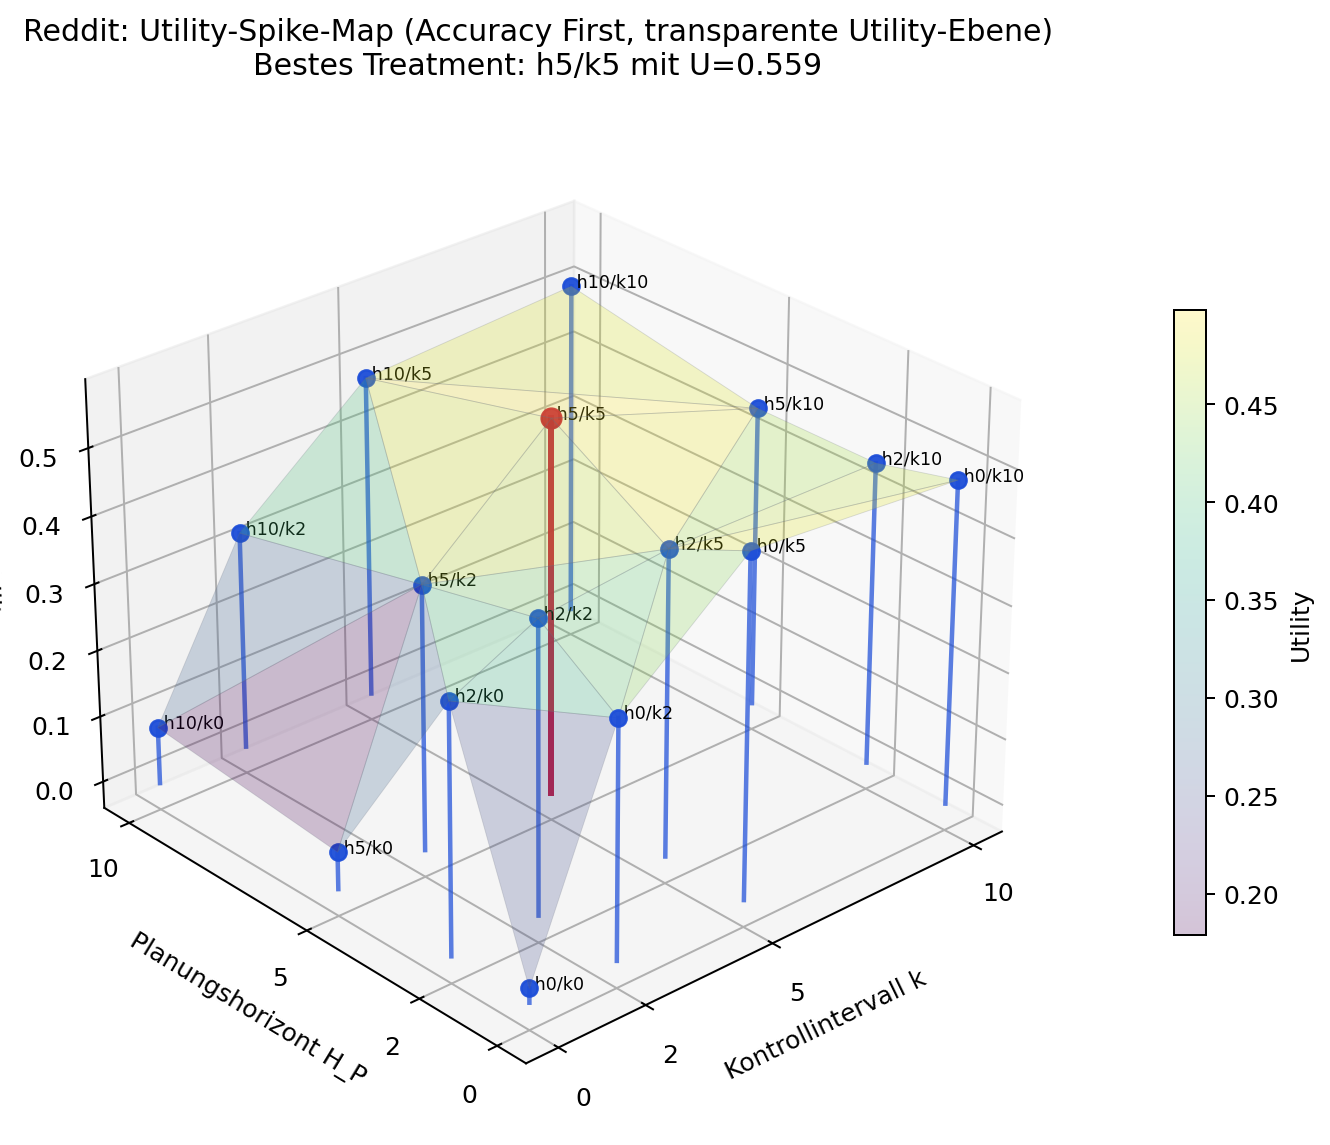
\includegraphics[width=\textwidth]
    {figures/fig_08_spike_transparent_reddit_accuracy_first.png}
    \caption{Reddit: Utility-Spike-Map mit transparenter Utility-Ebene für das Gewichtungsprofil Accuracy First}
    \label{fig:app-spike-transparent-reddit-accuracy-first}
\end{figure}

\begin{figure}[htbp]
    \centering
    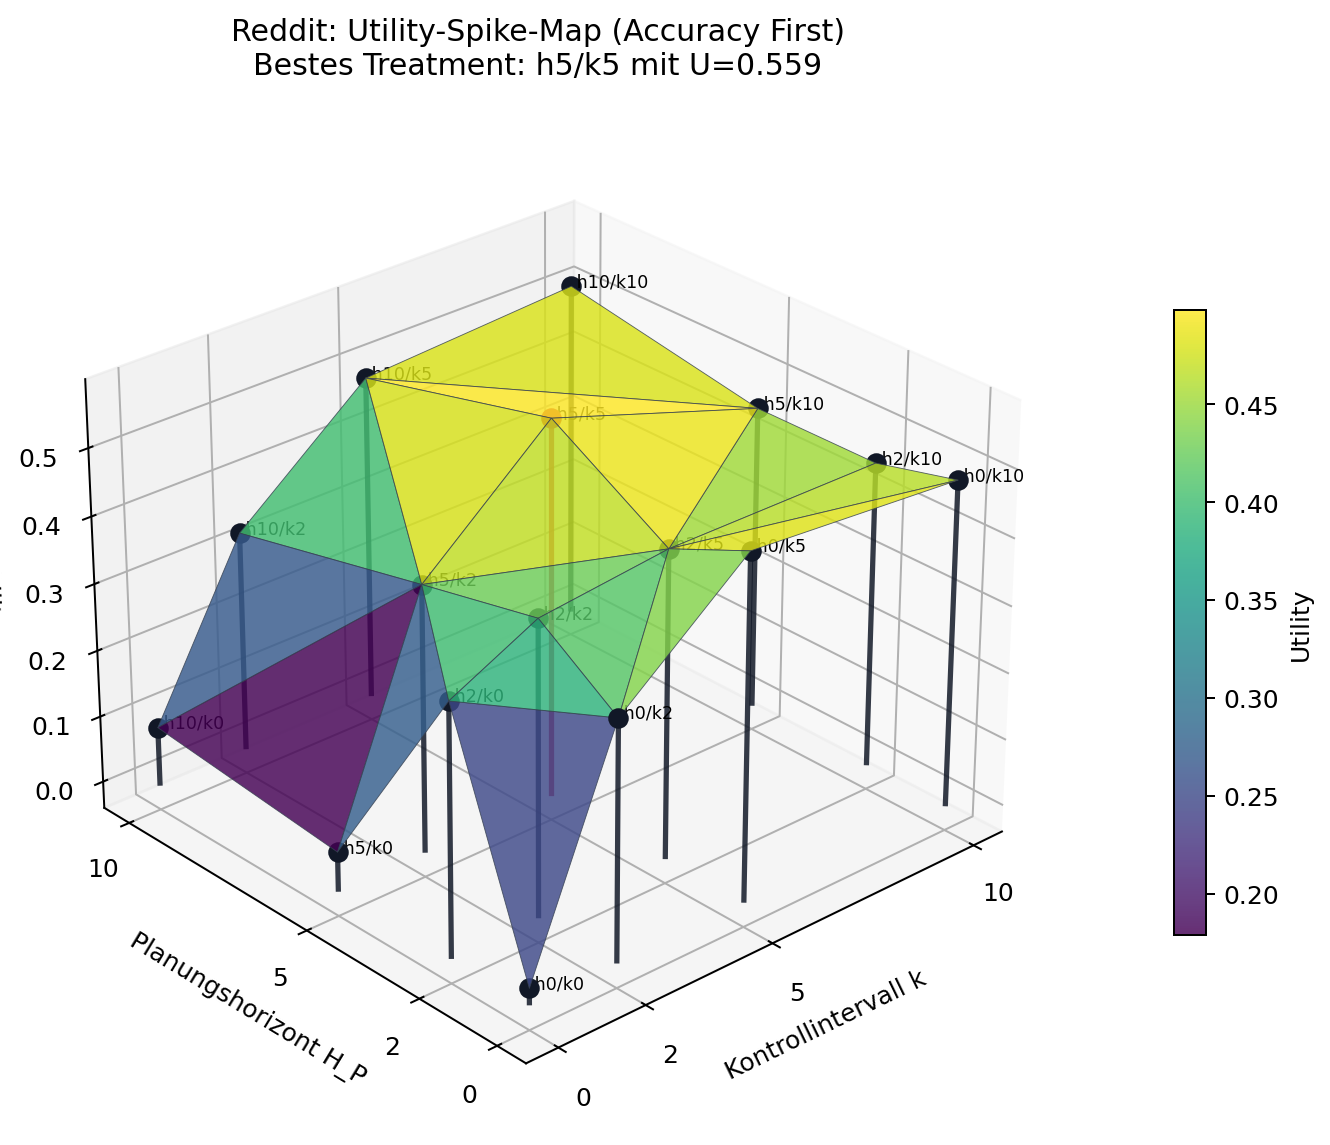
\includegraphics[width=\textwidth]
    {figures/fig_08_spike_reddit_accuracy_first.png}
    \caption{Reddit: Utility-Spike-Map mit kräftiger Utility-Ebene für das Gewichtungsprofil Accuracy First}
    \label{fig:app-spike-reddit-accuracy-first}
\end{figure}

\begin{figure}[htbp]
    \centering
    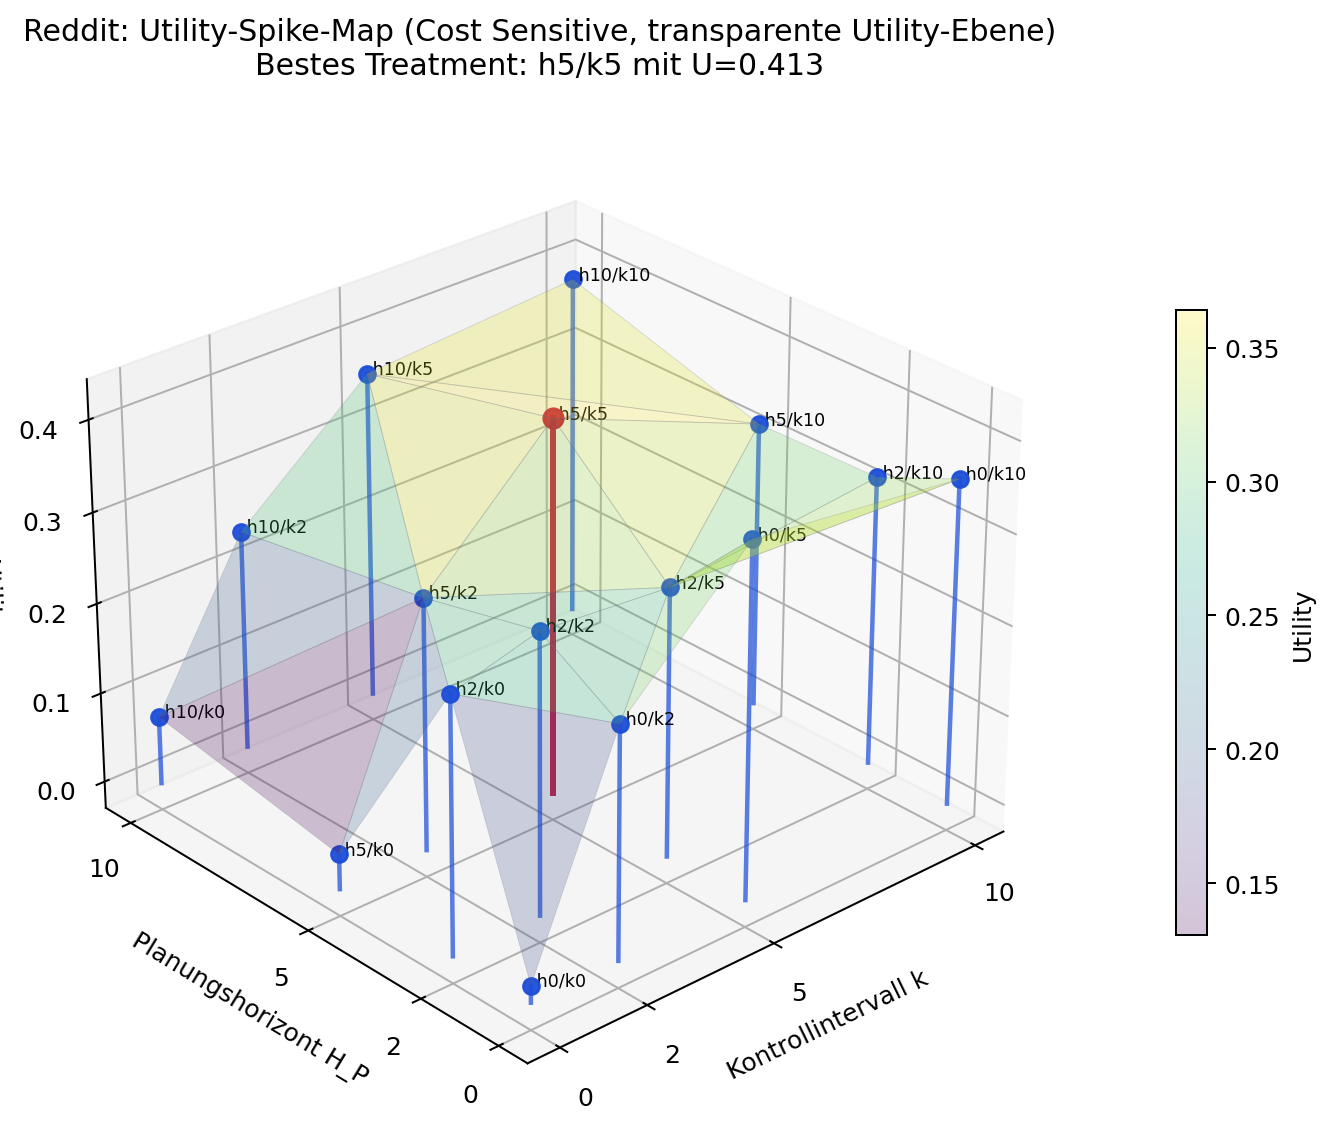
\includegraphics[width=\textwidth]
    {figures/fig_08_spike_transparent_reddit_cost_sensitive.png}
    \caption{Reddit: Utility-Spike-Map mit transparenter Utility-Ebene für das Gewichtungsprofil Cost Sensitive}
    \label{fig:app-spike-transparent-reddit-cost-sensitive}
\end{figure}

\begin{figure}[htbp]
    \centering
    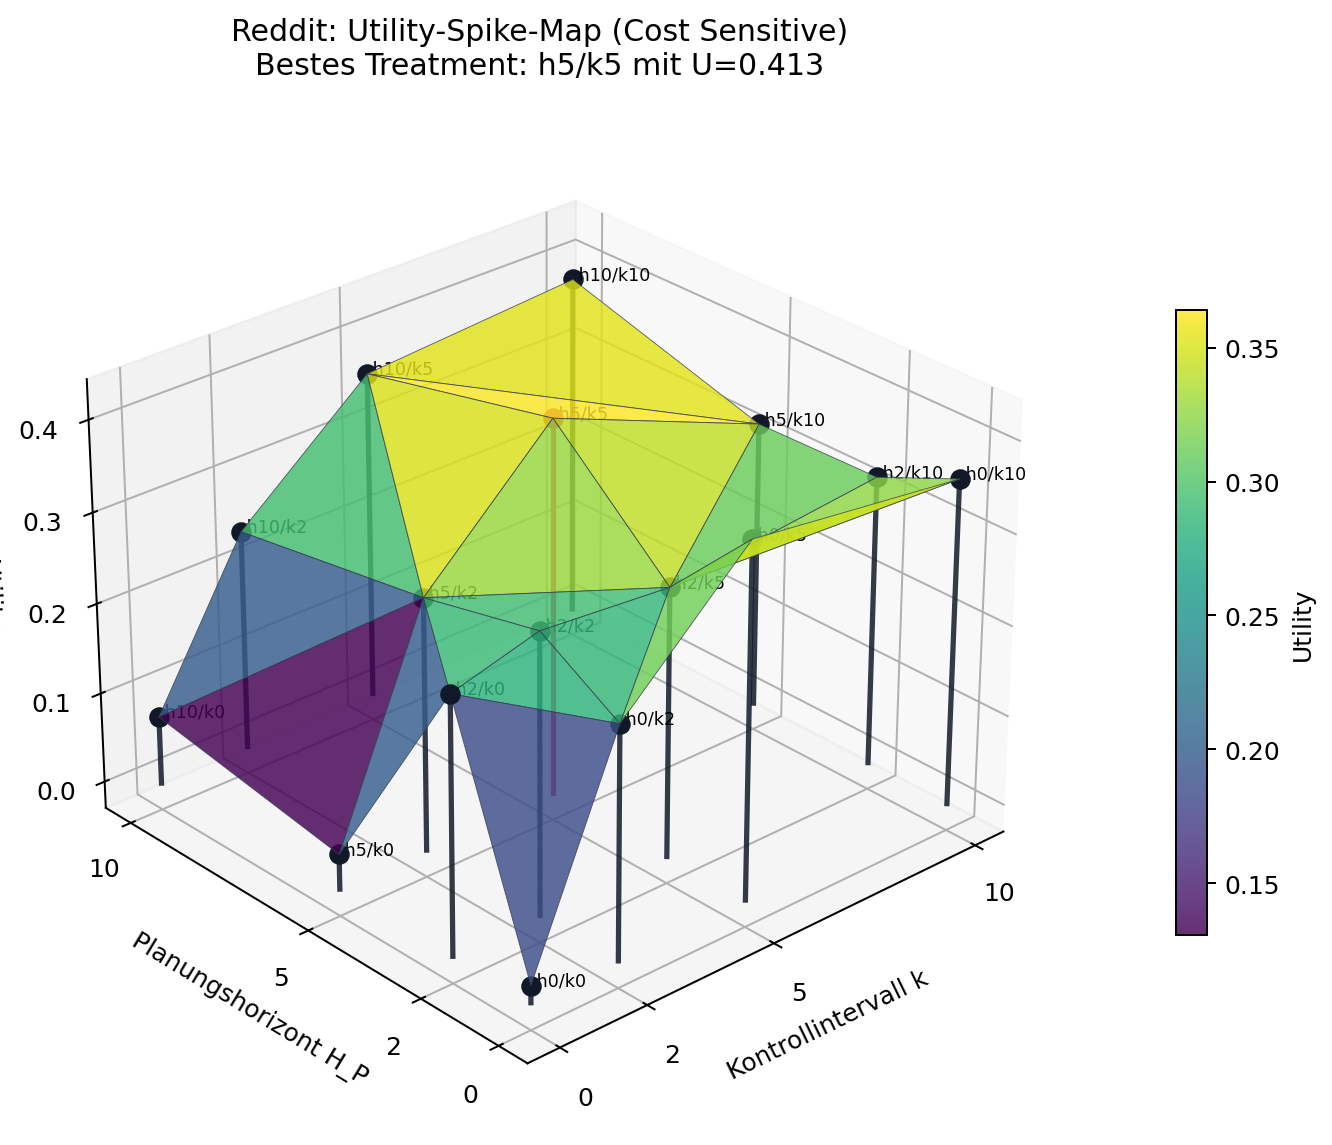
\includegraphics[width=\textwidth]
    {figures/fig_08_spike_reddit_cost_sensitive.png}
    \caption{Reddit: Utility-Spike-Map mit kräftiger Utility-Ebene für das Gewichtungsprofil Cost Sensitive}
    \label{fig:app-spike-reddit-cost-sensitive}
\end{figure}

\begin{figure}[htbp]
    \centering
    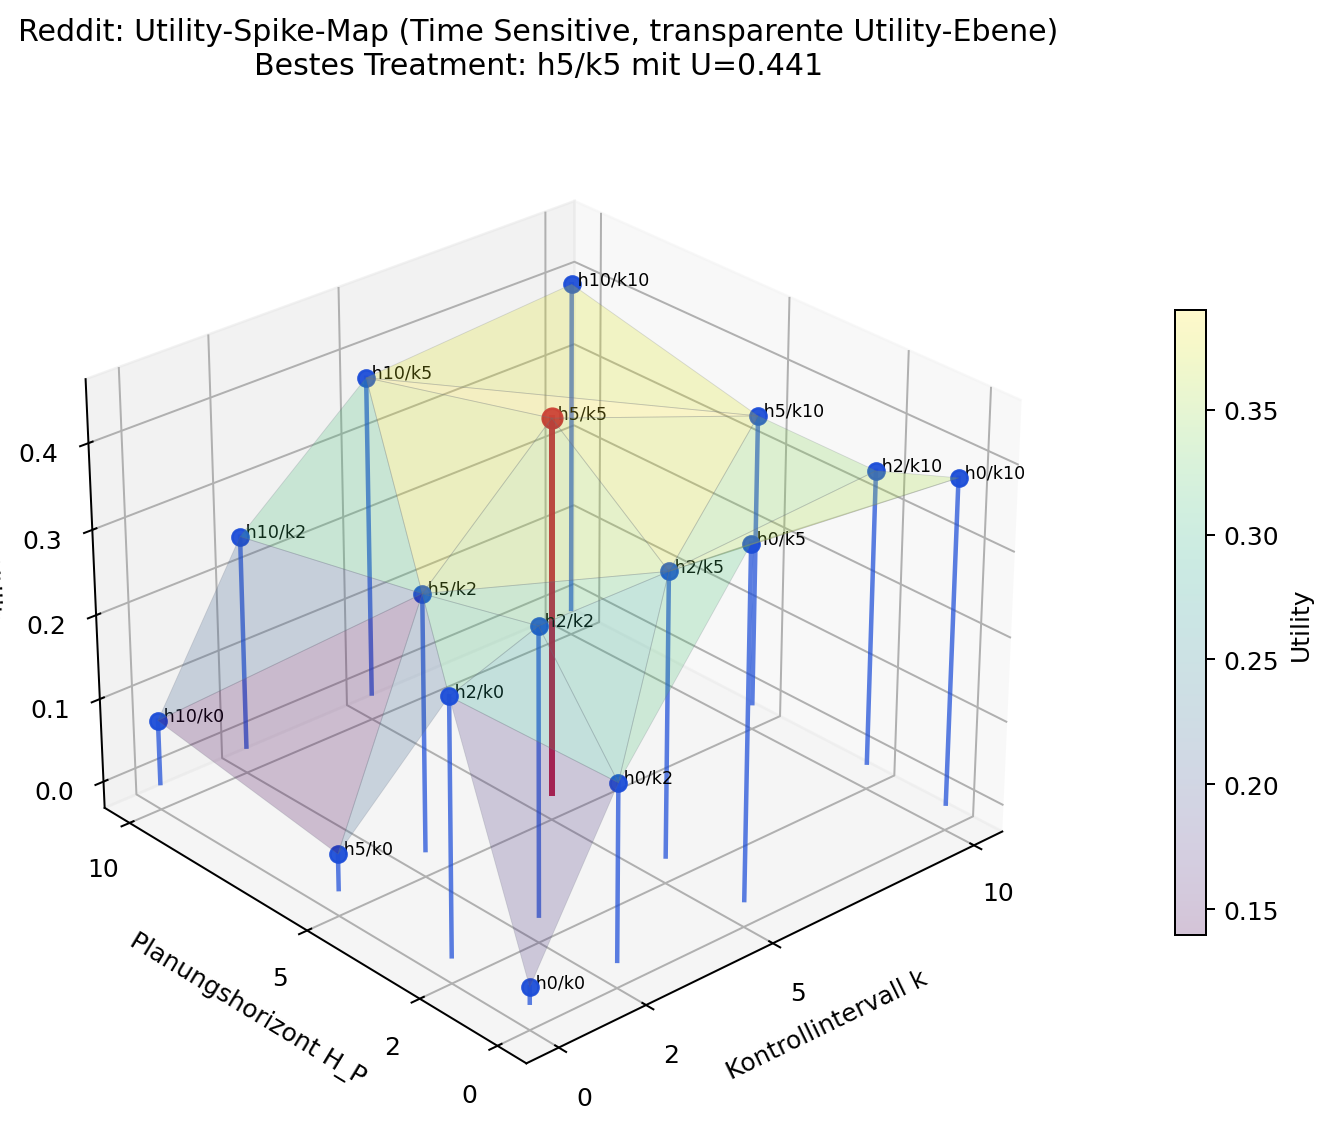
\includegraphics[width=\textwidth]
    {figures/fig_08_spike_transparent_reddit_time_sensitive.png}
    \caption{Reddit: Utility-Spike-Map mit transparenter Utility-Ebene für das Gewichtungsprofil Time Sensitive}
    \label{fig:app-spike-transparent-reddit-time-sensitive}
\end{figure}

\begin{figure}[htbp]
    \centering
    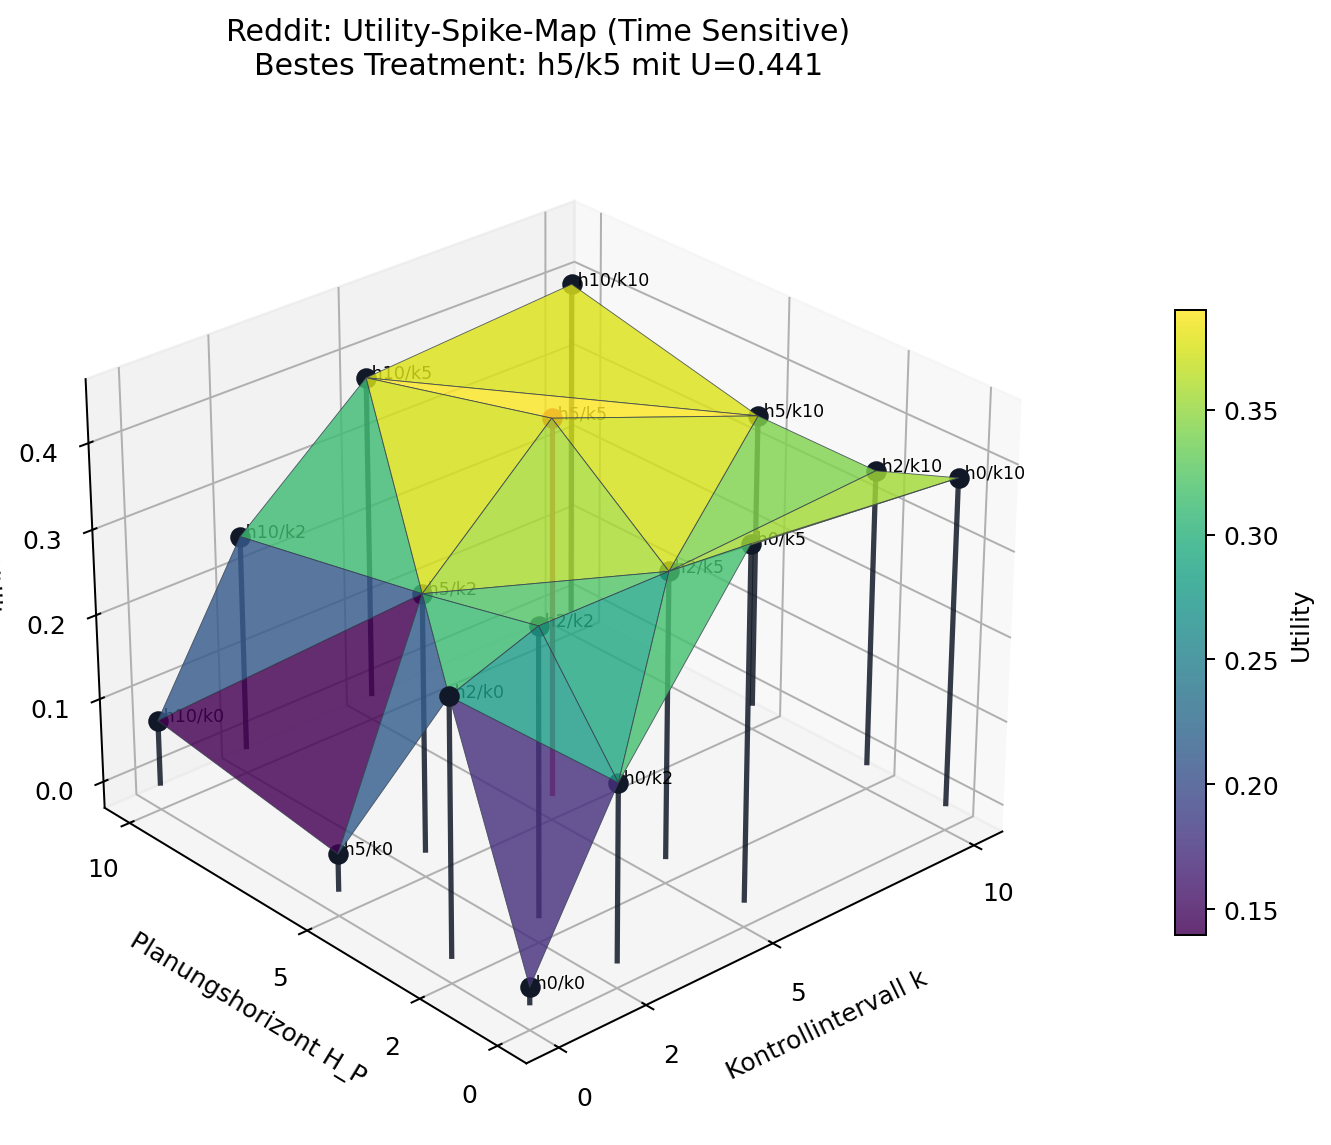
\includegraphics[width=\textwidth]
    {figures/fig_08_spike_reddit_time_sensitive.png}
    \caption{Reddit: Utility-Spike-Map mit kräftiger Utility-Ebene für das Gewichtungsprofil Time Sensitive}
    \label{fig:app-spike-reddit-time-sensitive}
\end{figure}

\begin{figure}[htbp]
    \centering
    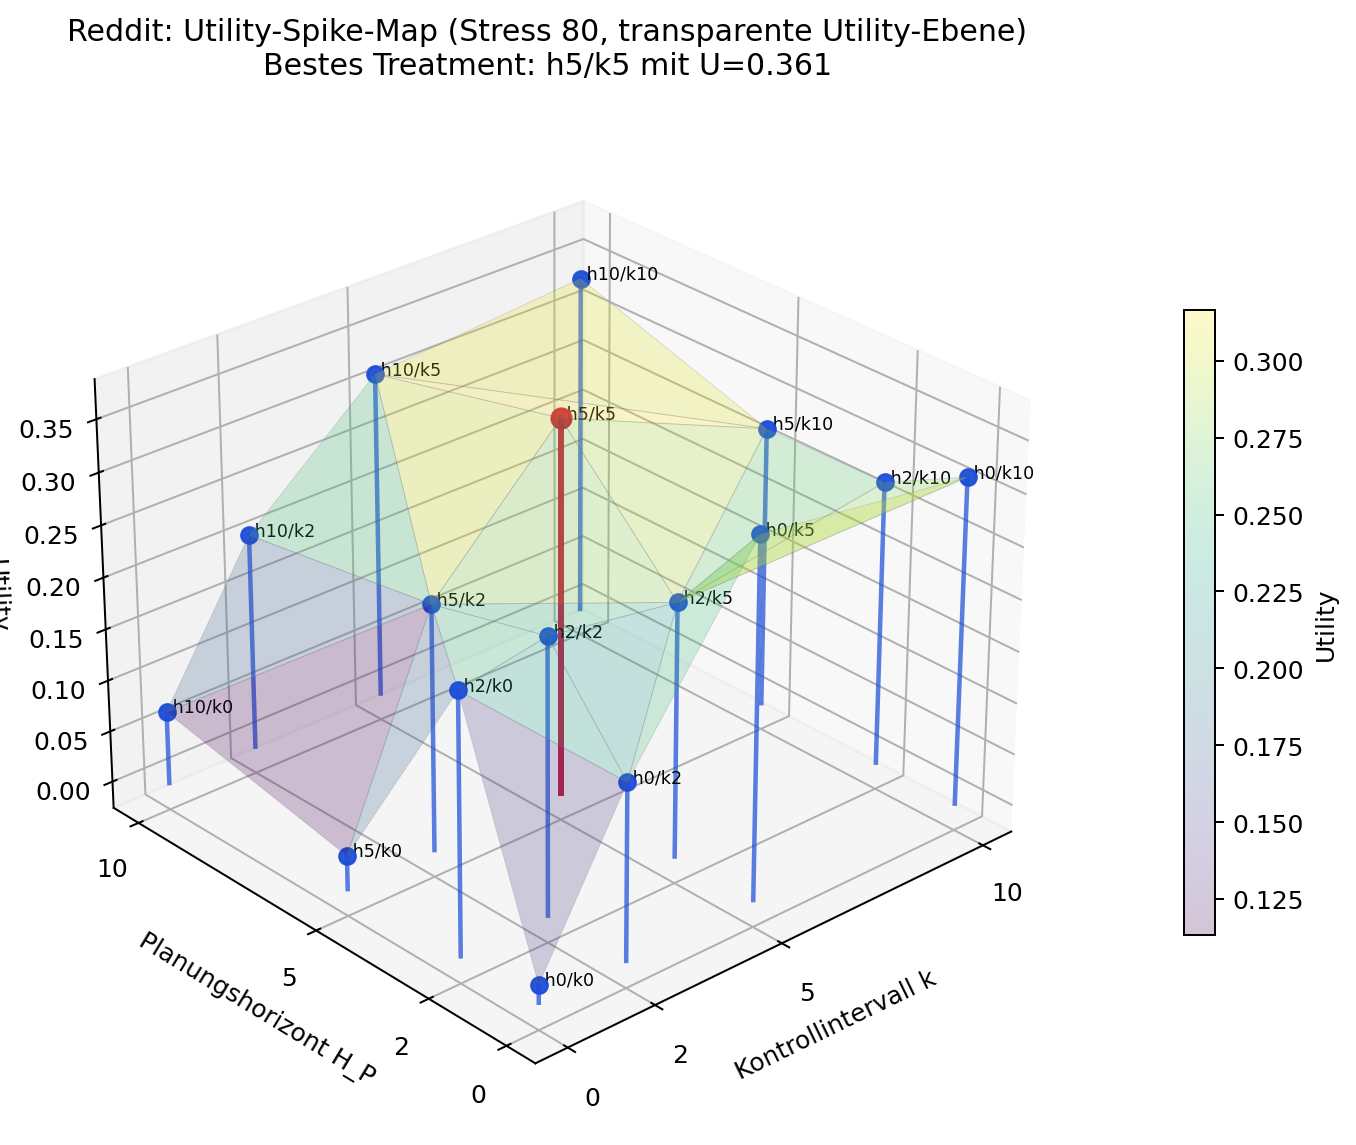
\includegraphics[width=\textwidth]
    {figures/fig_08_spike_transparent_reddit_stress_80.png}
    \caption{Reddit: Utility-Spike-Map mit transparenter Utility-Ebene für das Gewichtungsprofil Stress 80}
    \label{fig:app-spike-transparent-reddit-stress-80}
\end{figure}

\begin{figure}[htbp]
    \centering
    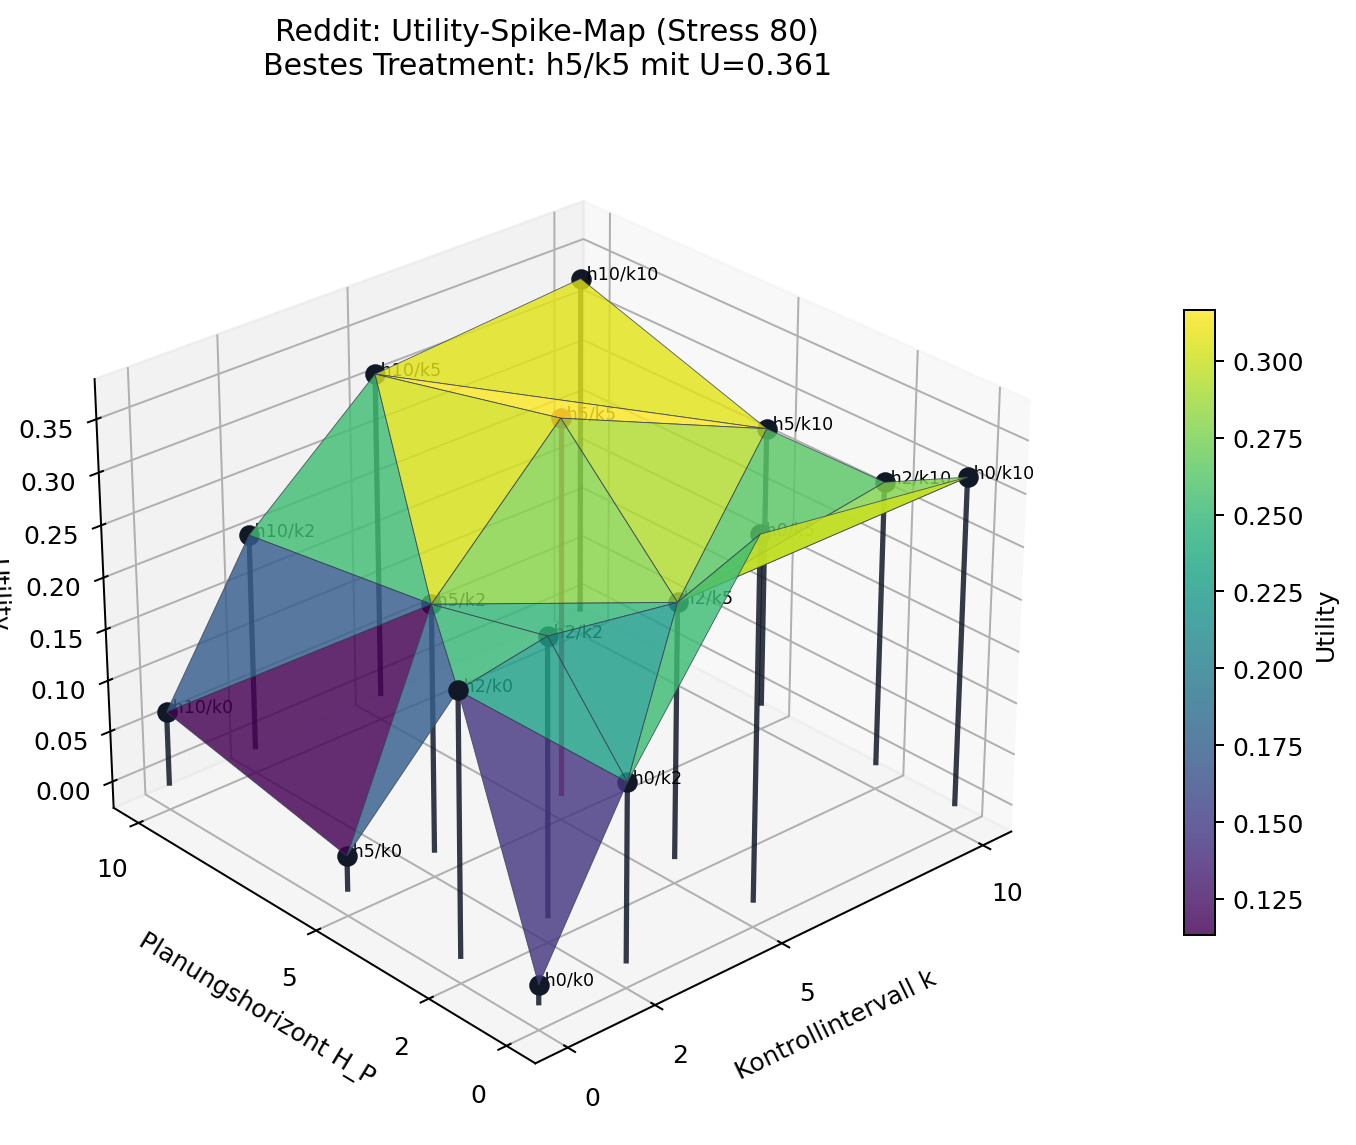
\includegraphics[width=\textwidth]
    {figures/fig_08_spike_reddit_stress_80.png}
    \caption{Reddit: Utility-Spike-Map mit kräftiger Utility-Ebene für das Gewichtungsprofil Stress 80}
    \label{fig:app-spike-reddit-stress-80}
\end{figure}

\clearpage
\subsubsection{Shopping}
\begin{figure}[htbp]
    \centering
    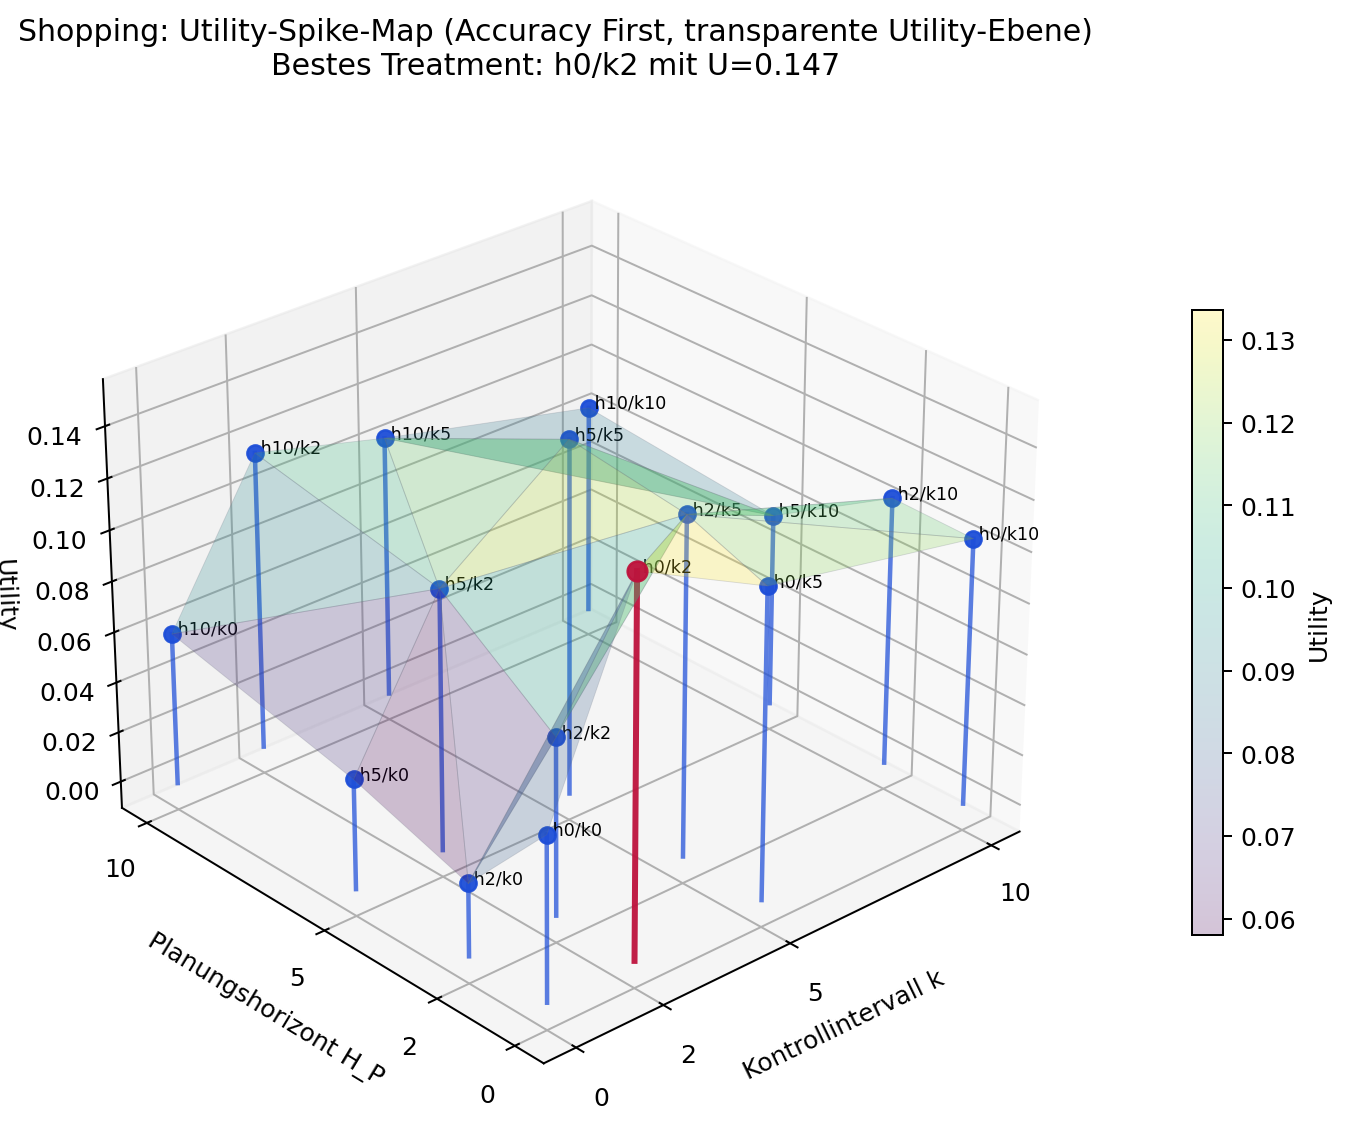
\includegraphics[width=\textwidth]
    {figures/fig_08_spike_transparent_shopping_accuracy_first.png}
    \caption{Shopping: Utility-Spike-Map mit transparenter Utility-Ebene für das Gewichtungsprofil Accuracy First}
    \label{fig:app-spike-transparent-shopping-accuracy-first}
\end{figure}

\begin{figure}[htbp]
    \centering
    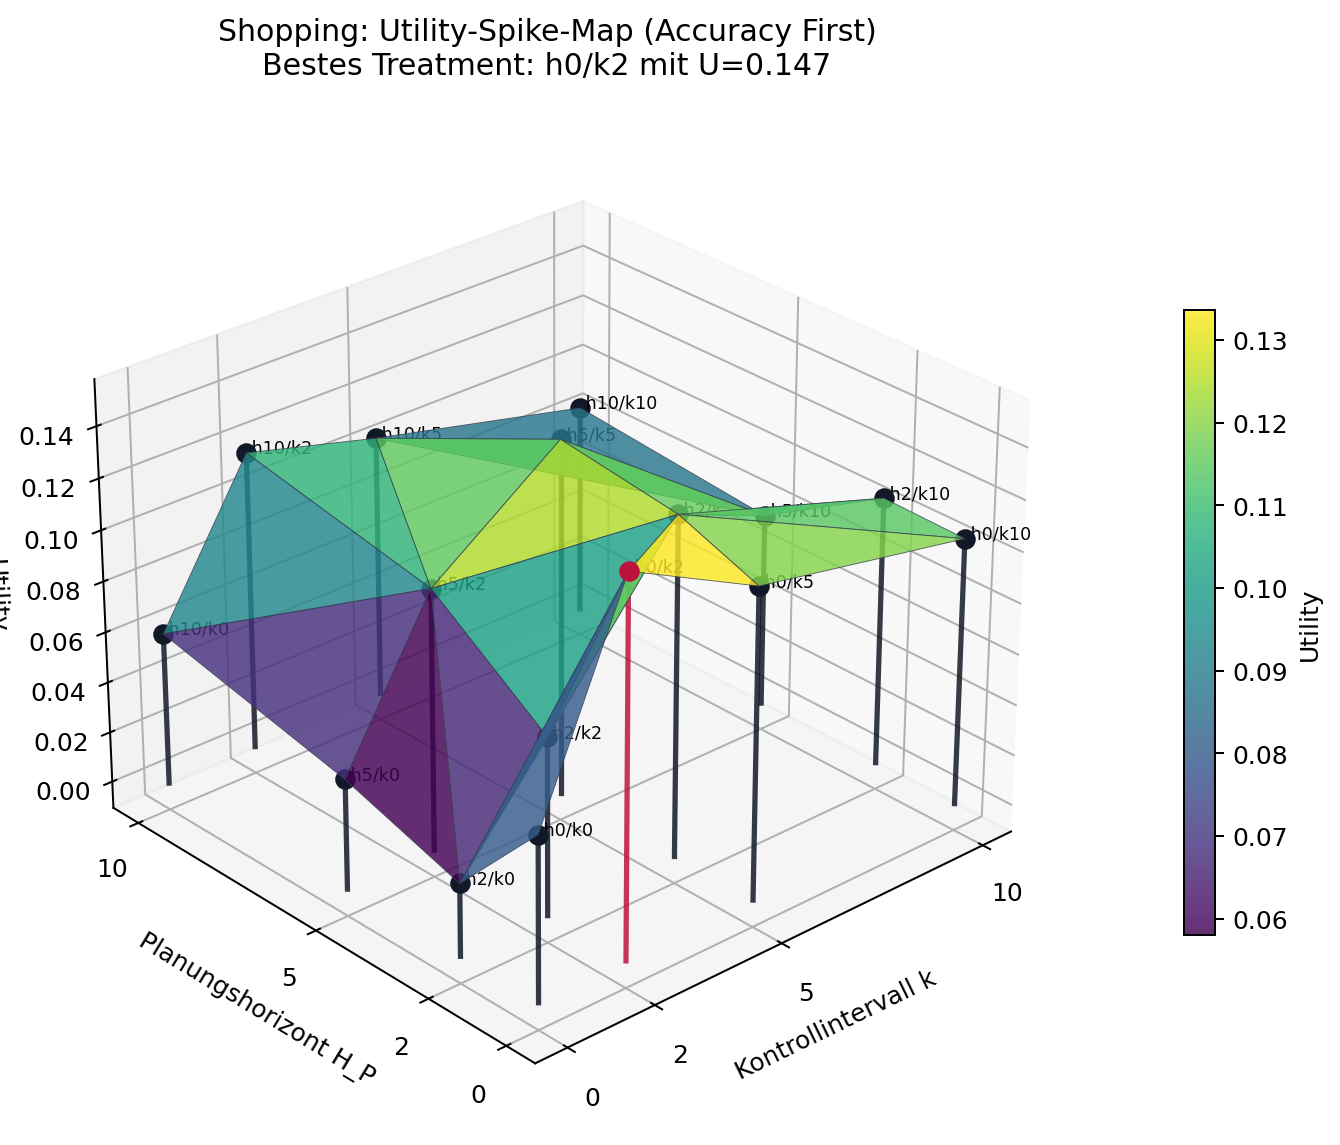
\includegraphics[width=\textwidth]
    {figures/fig_08_spike_shopping_accuracy_first.png}
    \caption{Shopping: Utility-Spike-Map mit kräftiger Utility-Ebene für das Gewichtungsprofil Accuracy First}
    \label{fig:app-spike-shopping-accuracy-first}
\end{figure}

\begin{figure}[htbp]
    \centering
    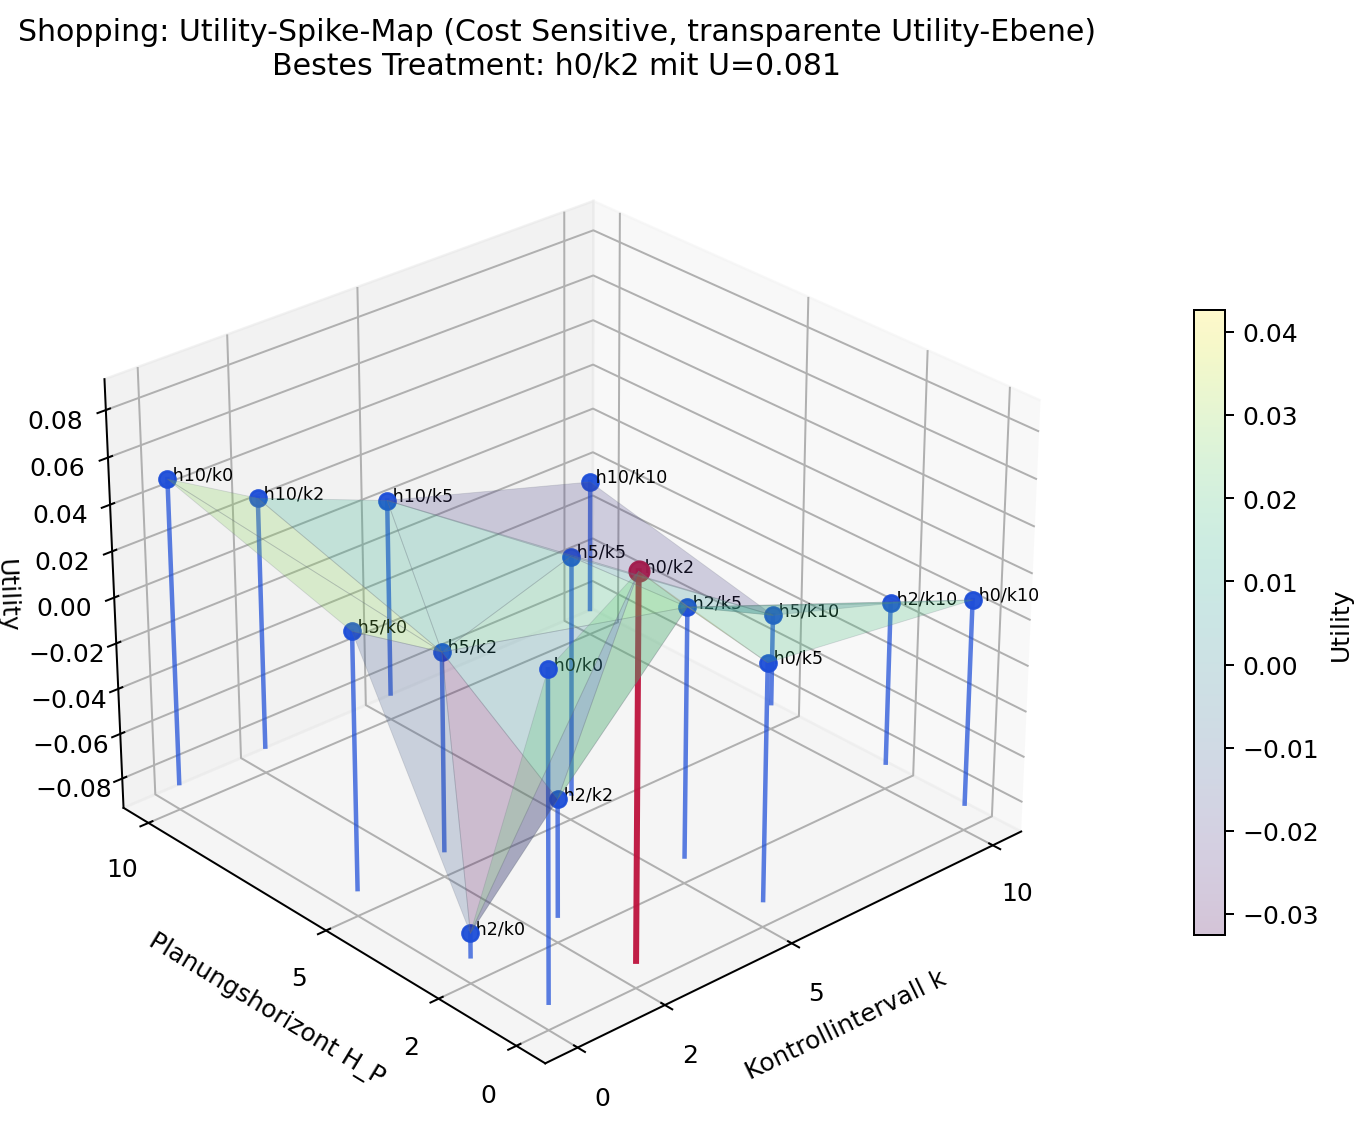
\includegraphics[width=\textwidth]
    {figures/fig_08_spike_transparent_shopping_cost_sensitive.png}
    \caption{Shopping: Utility-Spike-Map mit transparenter Utility-Ebene für das Gewichtungsprofil Cost Sensitive}
    \label{fig:app-spike-transparent-shopping-cost-sensitive}
\end{figure}

\begin{figure}[htbp]
    \centering
    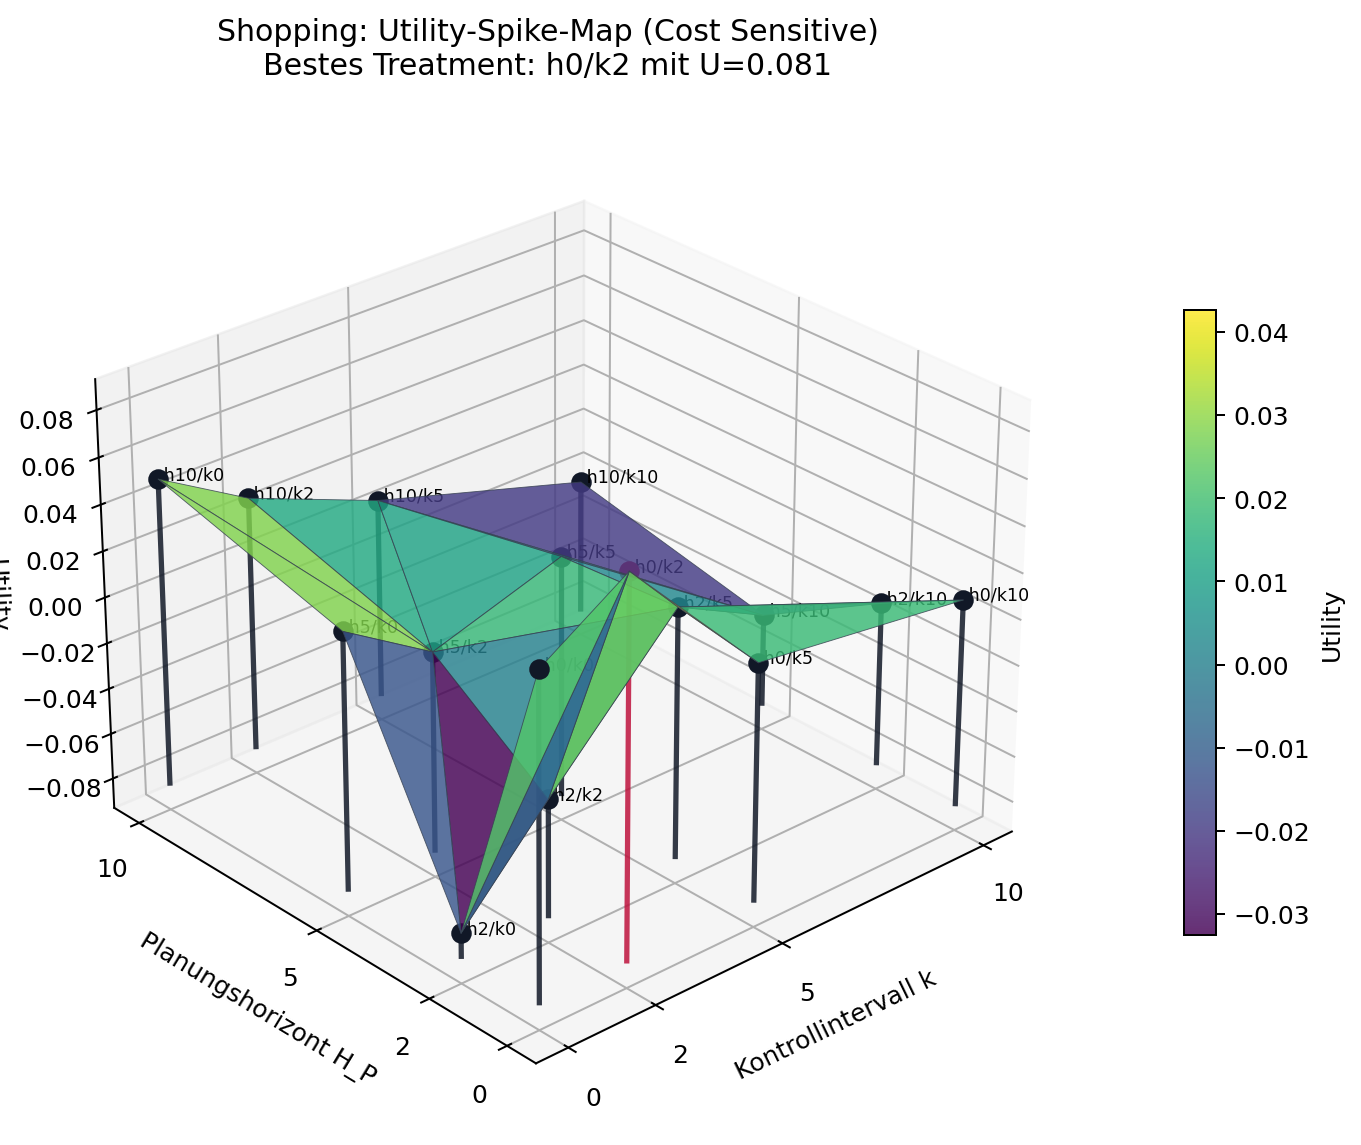
\includegraphics[width=\textwidth]
    {figures/fig_08_spike_shopping_cost_sensitive.png}
    \caption{Shopping: Utility-Spike-Map mit kräftiger Utility-Ebene für das Gewichtungsprofil Cost Sensitive}
    \label{fig:app-spike-shopping-cost-sensitive}
\end{figure}

\begin{figure}[htbp]
    \centering
    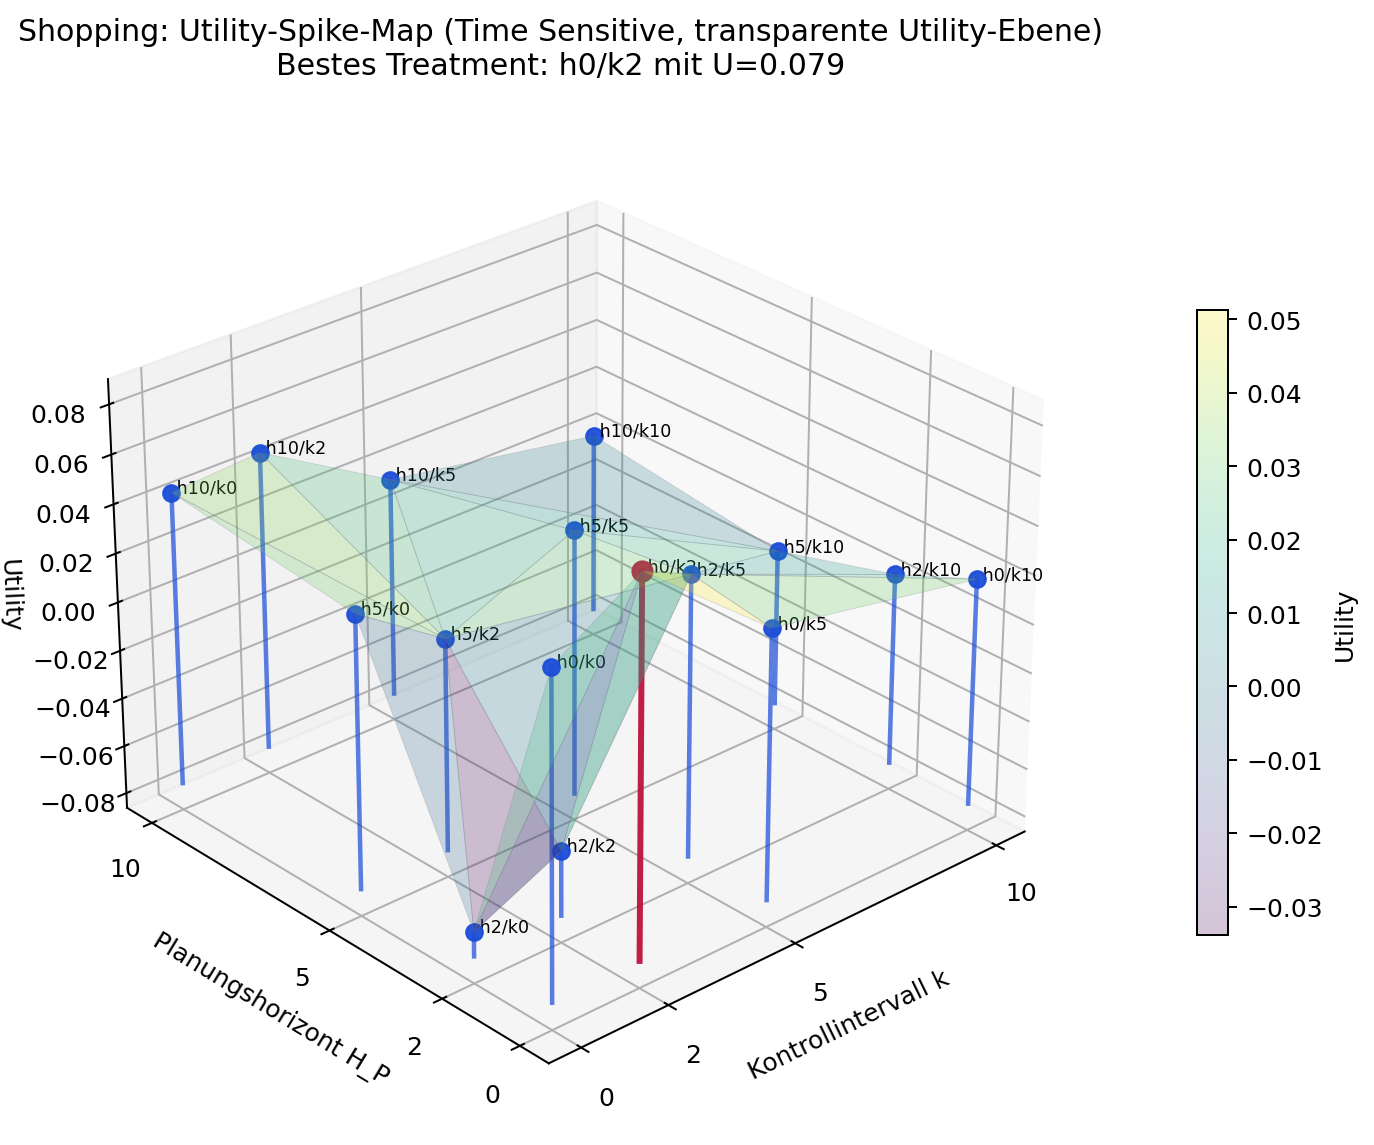
\includegraphics[width=\textwidth]
    {figures/fig_08_spike_transparent_shopping_time_sensitive.png}
    \caption{Shopping: Utility-Spike-Map mit transparenter Utility-Ebene für das Gewichtungsprofil Time Sensitive}
    \label{fig:app-spike-transparent-shopping-time-sensitive}
\end{figure}

\begin{figure}[htbp]
    \centering
    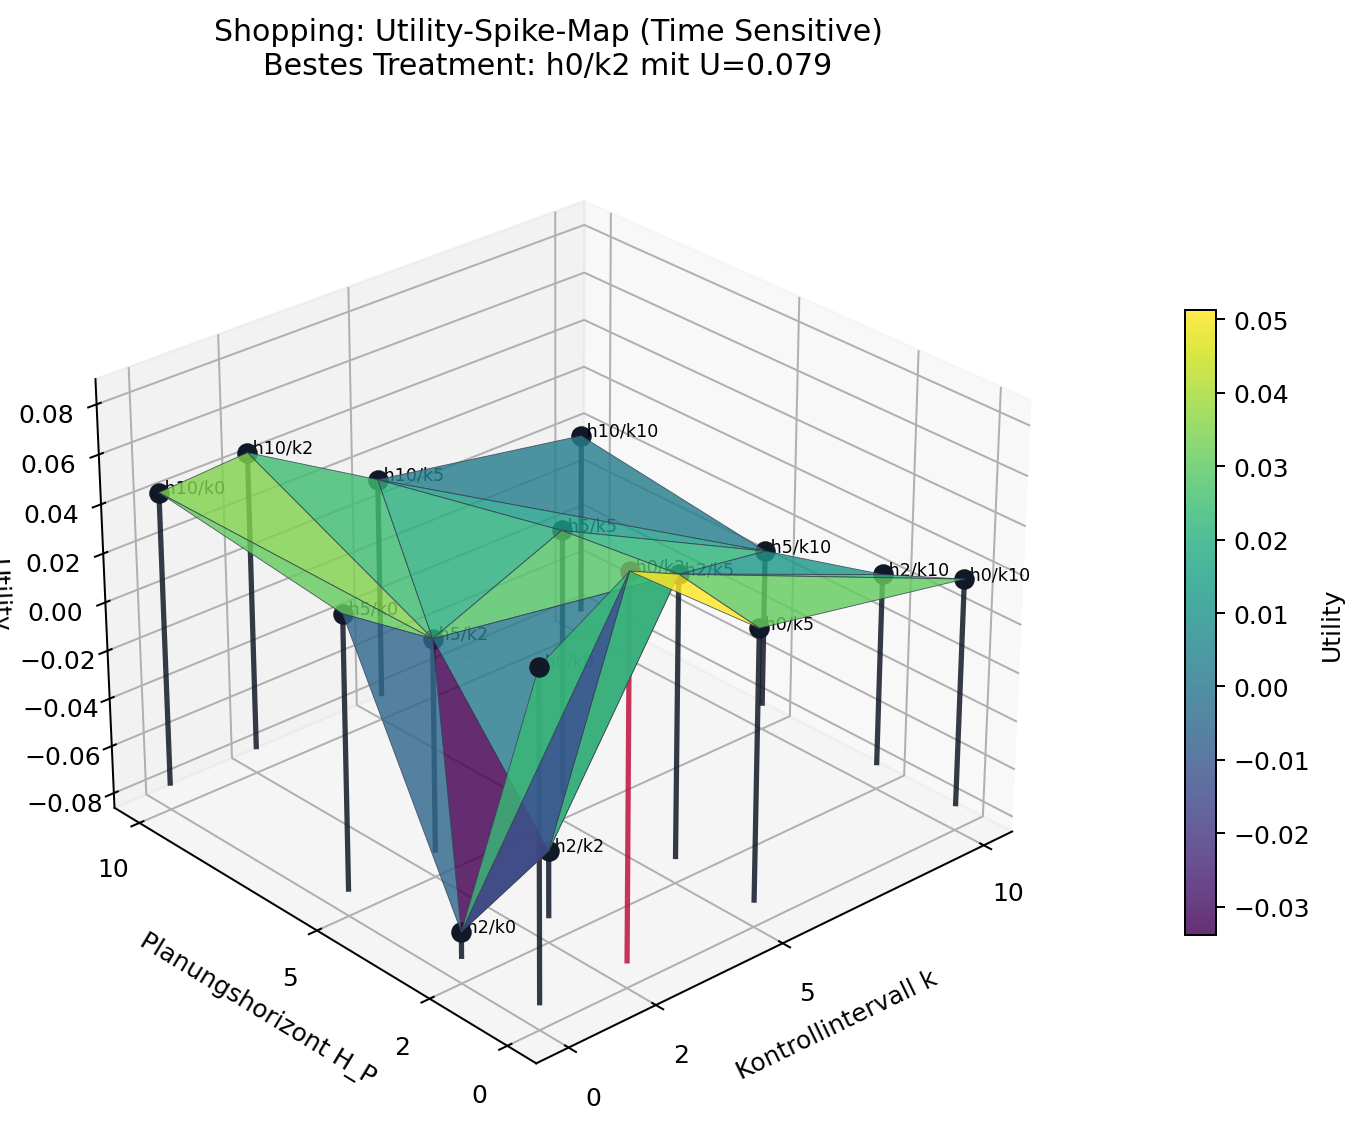
\includegraphics[width=\textwidth]
    {figures/fig_08_spike_shopping_time_sensitive.png}
    \caption{Shopping: Utility-Spike-Map mit kräftiger Utility-Ebene für das Gewichtungsprofil Time Sensitive}
    \label{fig:app-spike-shopping-time-sensitive}
\end{figure}

\begin{figure}[htbp]
    \centering
    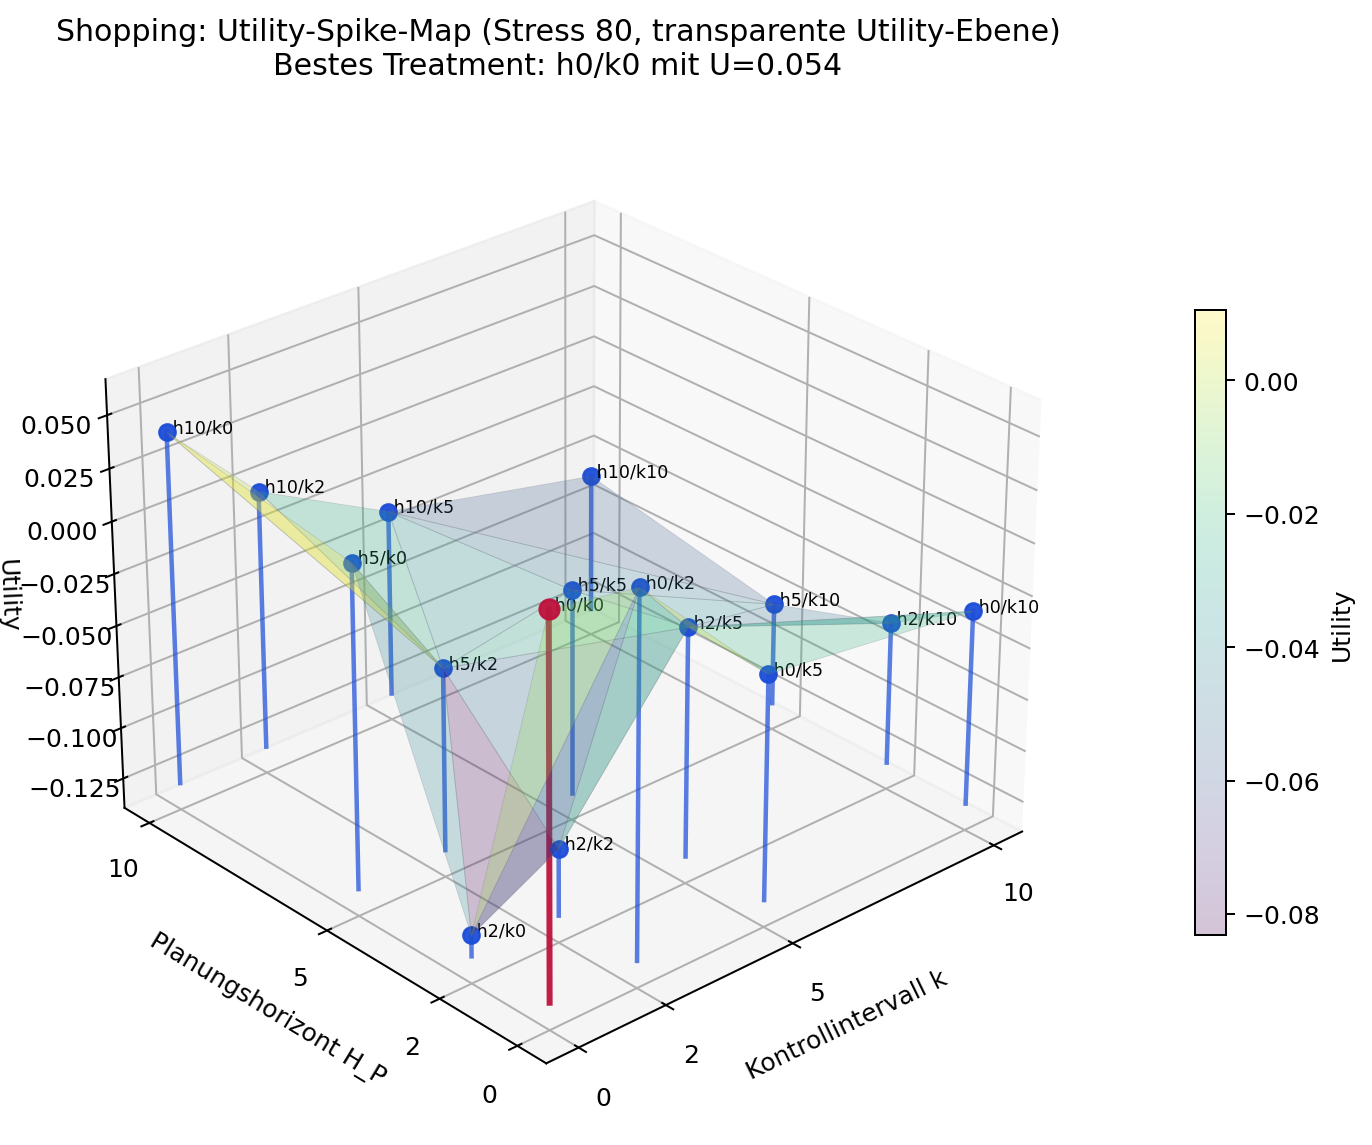
\includegraphics[width=\textwidth]
    {figures/fig_08_spike_transparent_shopping_stress_80.png}
    \caption{Shopping: Utility-Spike-Map mit transparenter Utility-Ebene für das Gewichtungsprofil Stress 80}
    \label{fig:app-spike-transparent-shopping-stress-80}
\end{figure}

\begin{figure}[htbp]
    \centering
    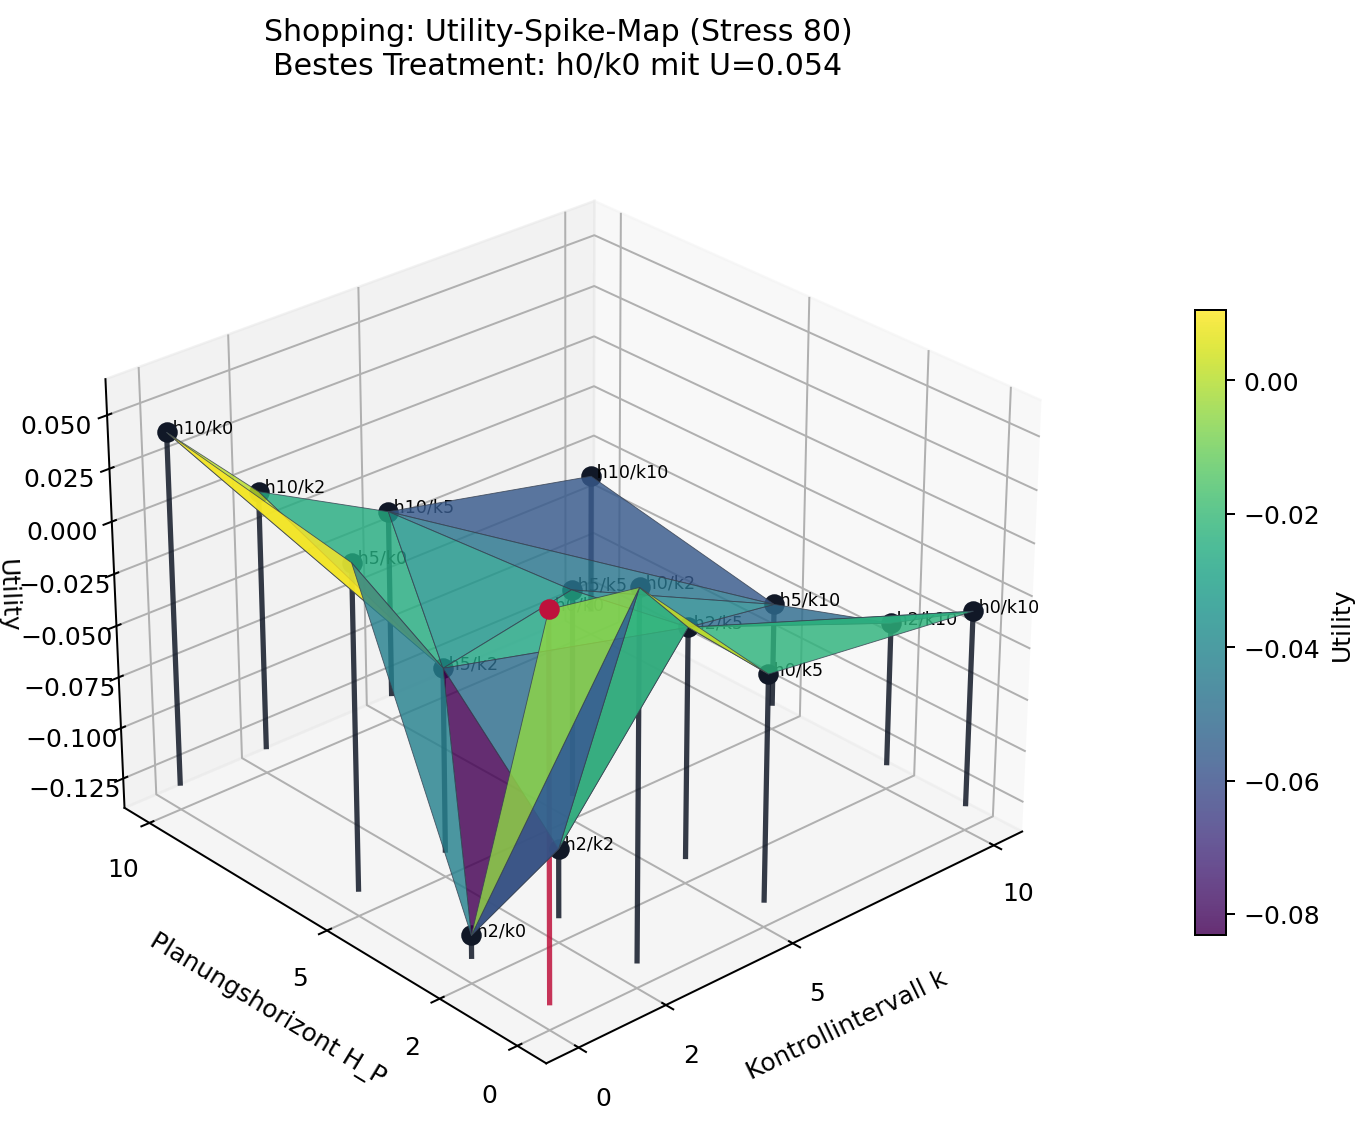
\includegraphics[width=\textwidth]
    {figures/fig_08_spike_shopping_stress_80.png}
    \caption{Shopping: Utility-Spike-Map mit kräftiger Utility-Ebene für das Gewichtungsprofil Stress 80}
    \label{fig:app-spike-shopping-stress-80}
\end{figure}

\clearpage
\subsubsection{Shopping Admin}
\begin{figure}[htbp]
    \centering
    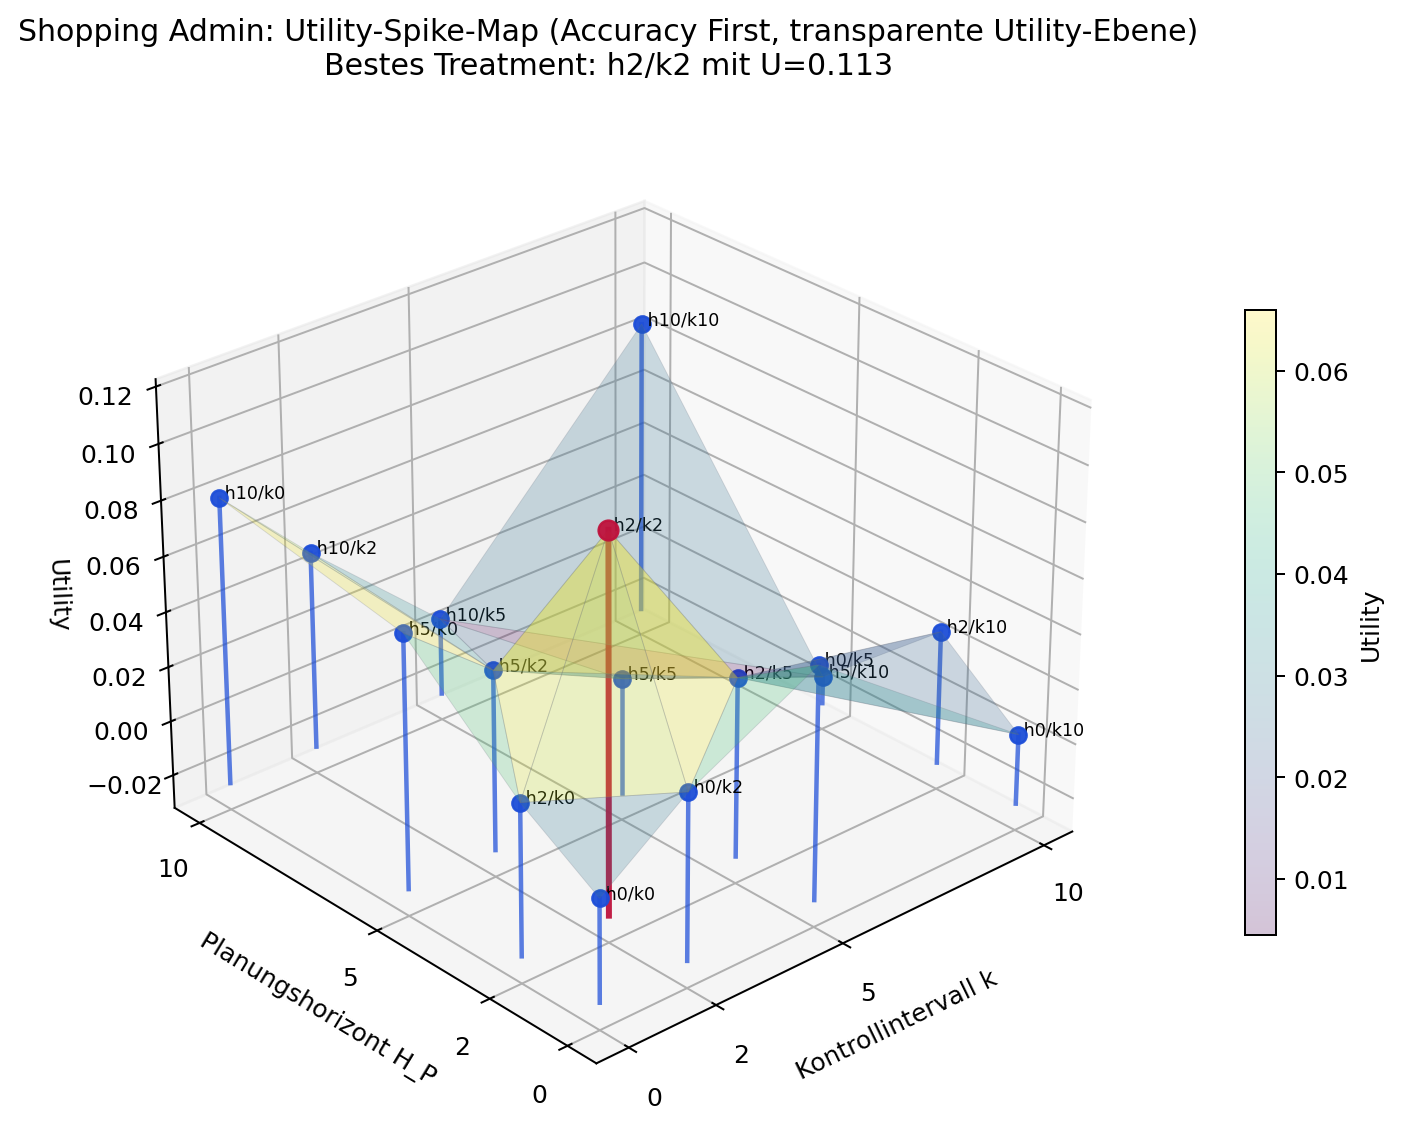
\includegraphics[width=\textwidth]
    {figures/fig_08_spike_transparent_shopping_admin_accuracy_first.png}
    \caption{Shopping Admin: Utility-Spike-Map mit transparenter Utility-Ebene für das Gewichtungsprofil Accuracy First}
    \label{fig:app-spike-transparent-shopping-admin-accuracy-first}
\end{figure}

\begin{figure}[htbp]
    \centering
    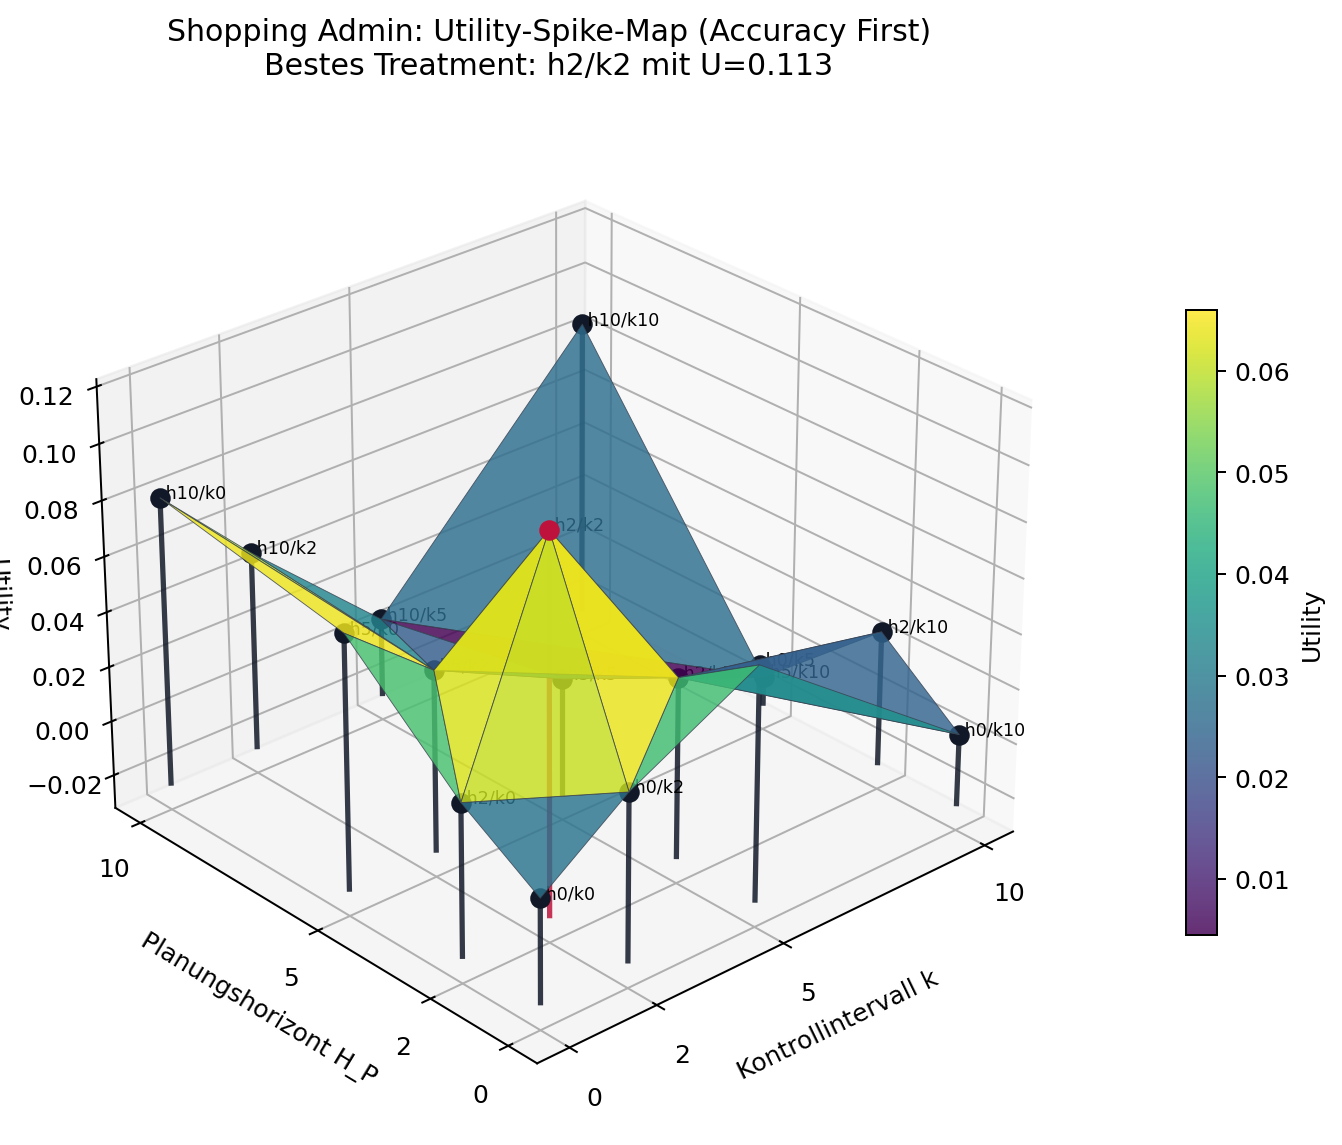
\includegraphics[width=\textwidth]
    {figures/fig_08_spike_shopping_admin_accuracy_first.png}
    \caption{Shopping Admin: Utility-Spike-Map mit kräftiger Utility-Ebene für das Gewichtungsprofil Accuracy First}
    \label{fig:app-spike-shopping-admin-accuracy-first}
\end{figure}

\begin{figure}[htbp]
    \centering
    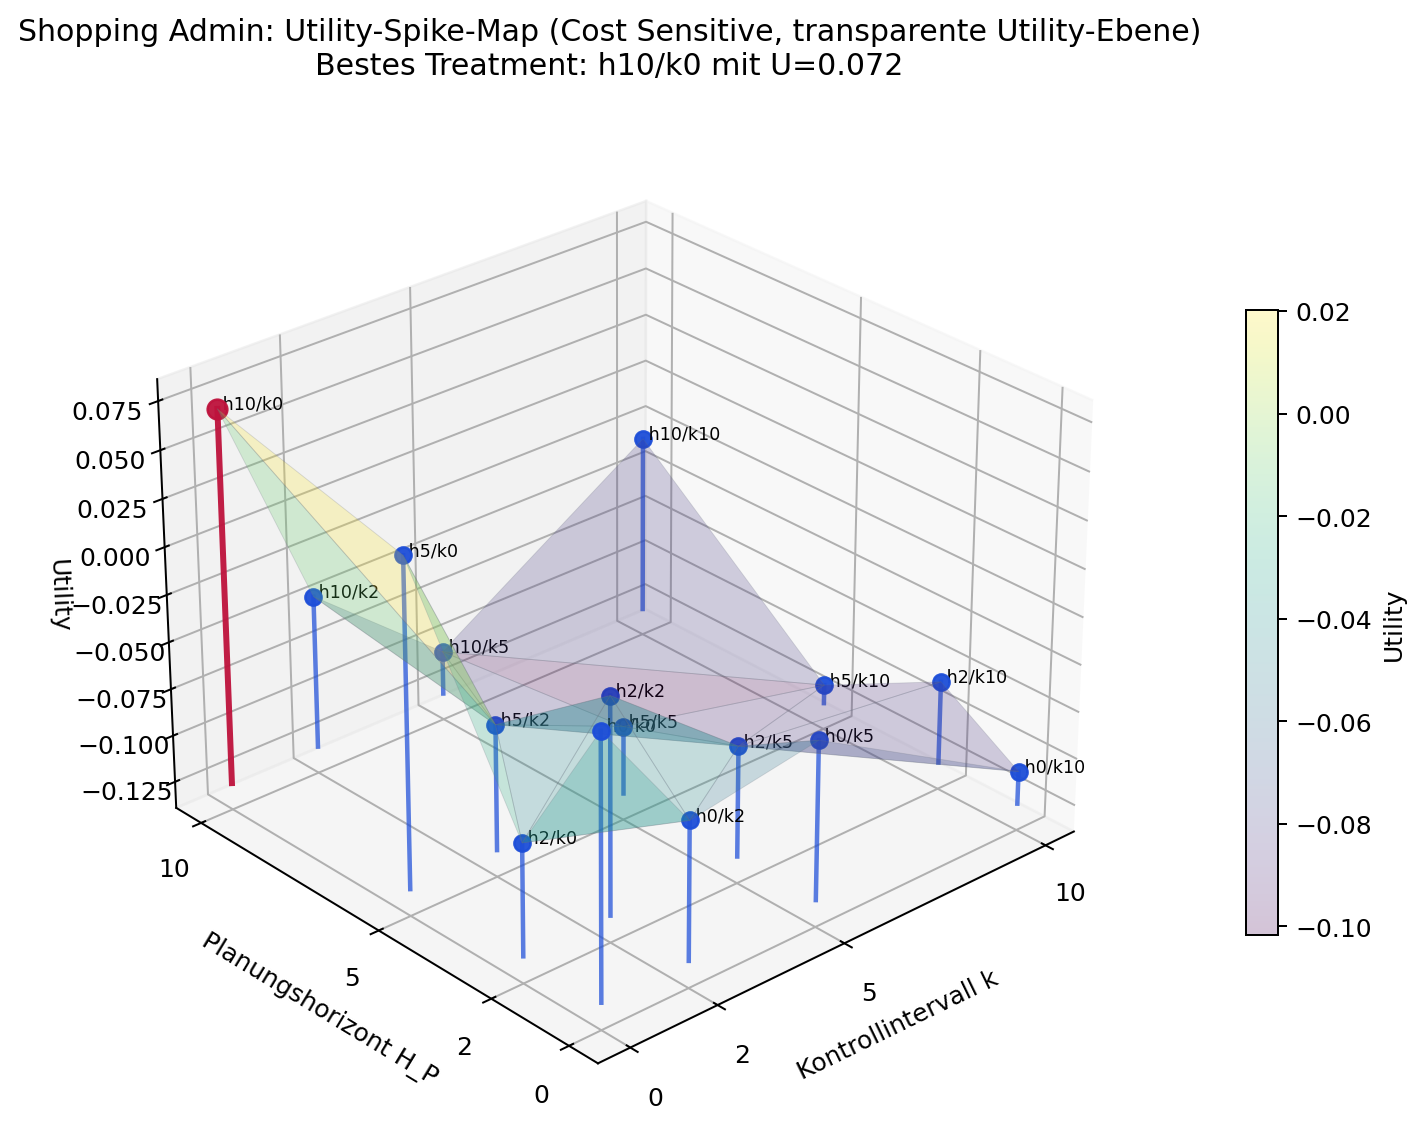
\includegraphics[width=\textwidth]
    {figures/fig_08_spike_transparent_shopping_admin_cost_sensitive.png}
    \caption{Shopping Admin: Utility-Spike-Map mit transparenter Utility-Ebene für das Gewichtungsprofil Cost Sensitive}
    \label{fig:app-spike-transparent-shopping-admin-cost-sensitive}
\end{figure}

\begin{figure}[htbp]
    \centering
    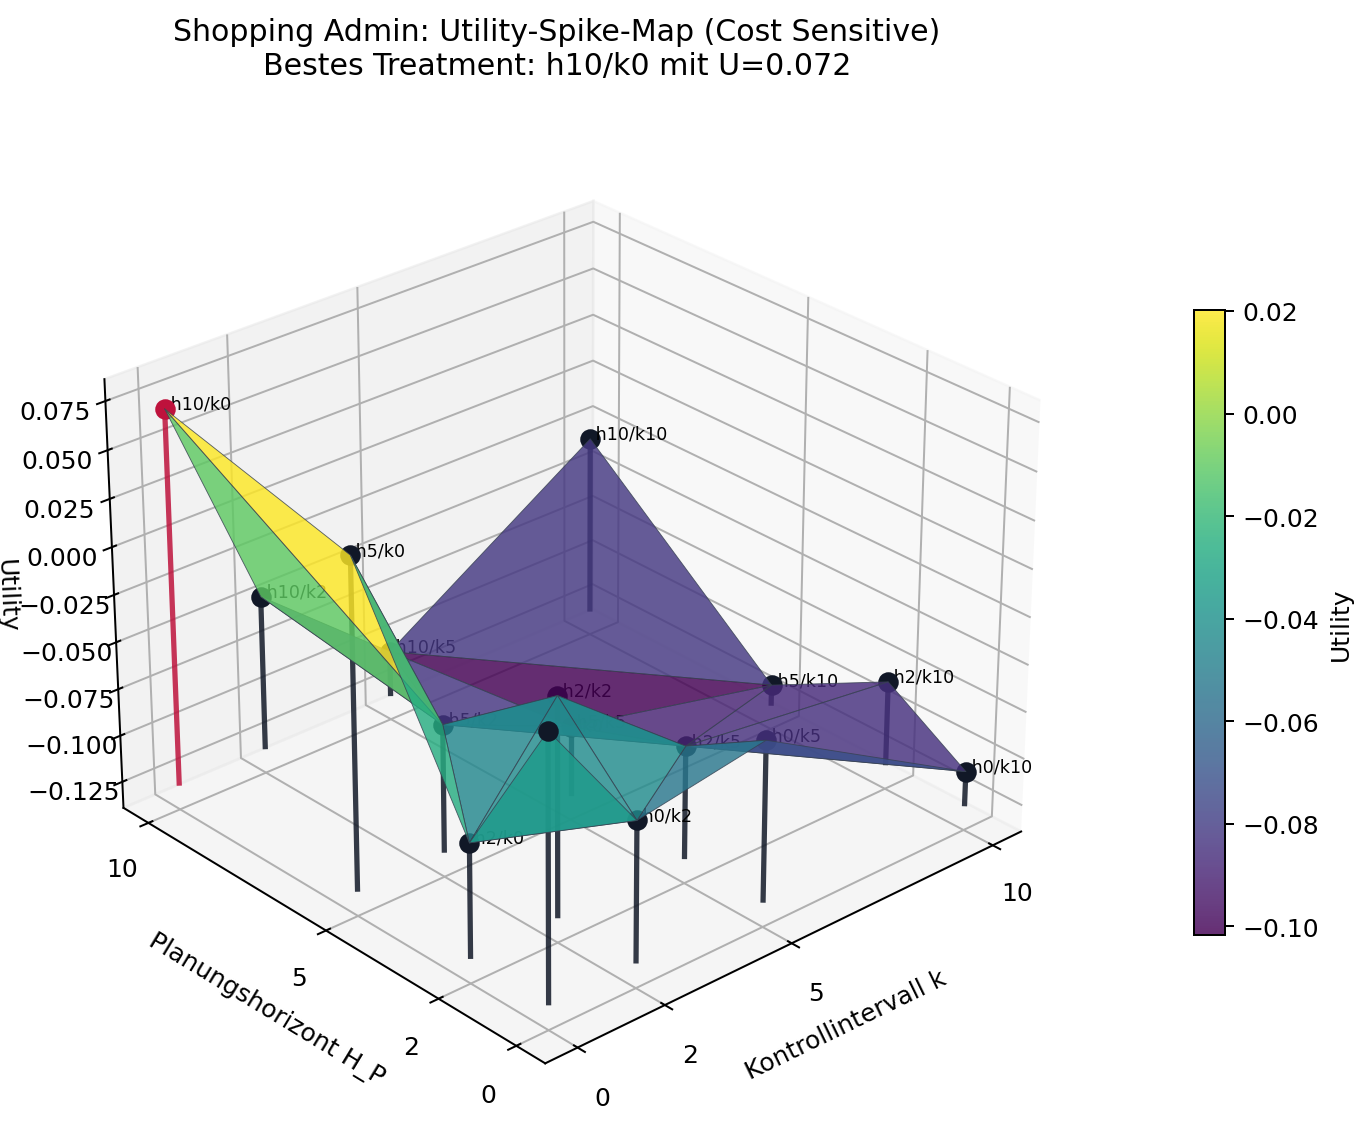
\includegraphics[width=\textwidth]
    {figures/fig_08_spike_shopping_admin_cost_sensitive.png}
    \caption{Shopping Admin: Utility-Spike-Map mit kräftiger Utility-Ebene für das Gewichtungsprofil Cost Sensitive}
    \label{fig:app-spike-shopping-admin-cost-sensitive}
\end{figure}

\begin{figure}[htbp]
    \centering
    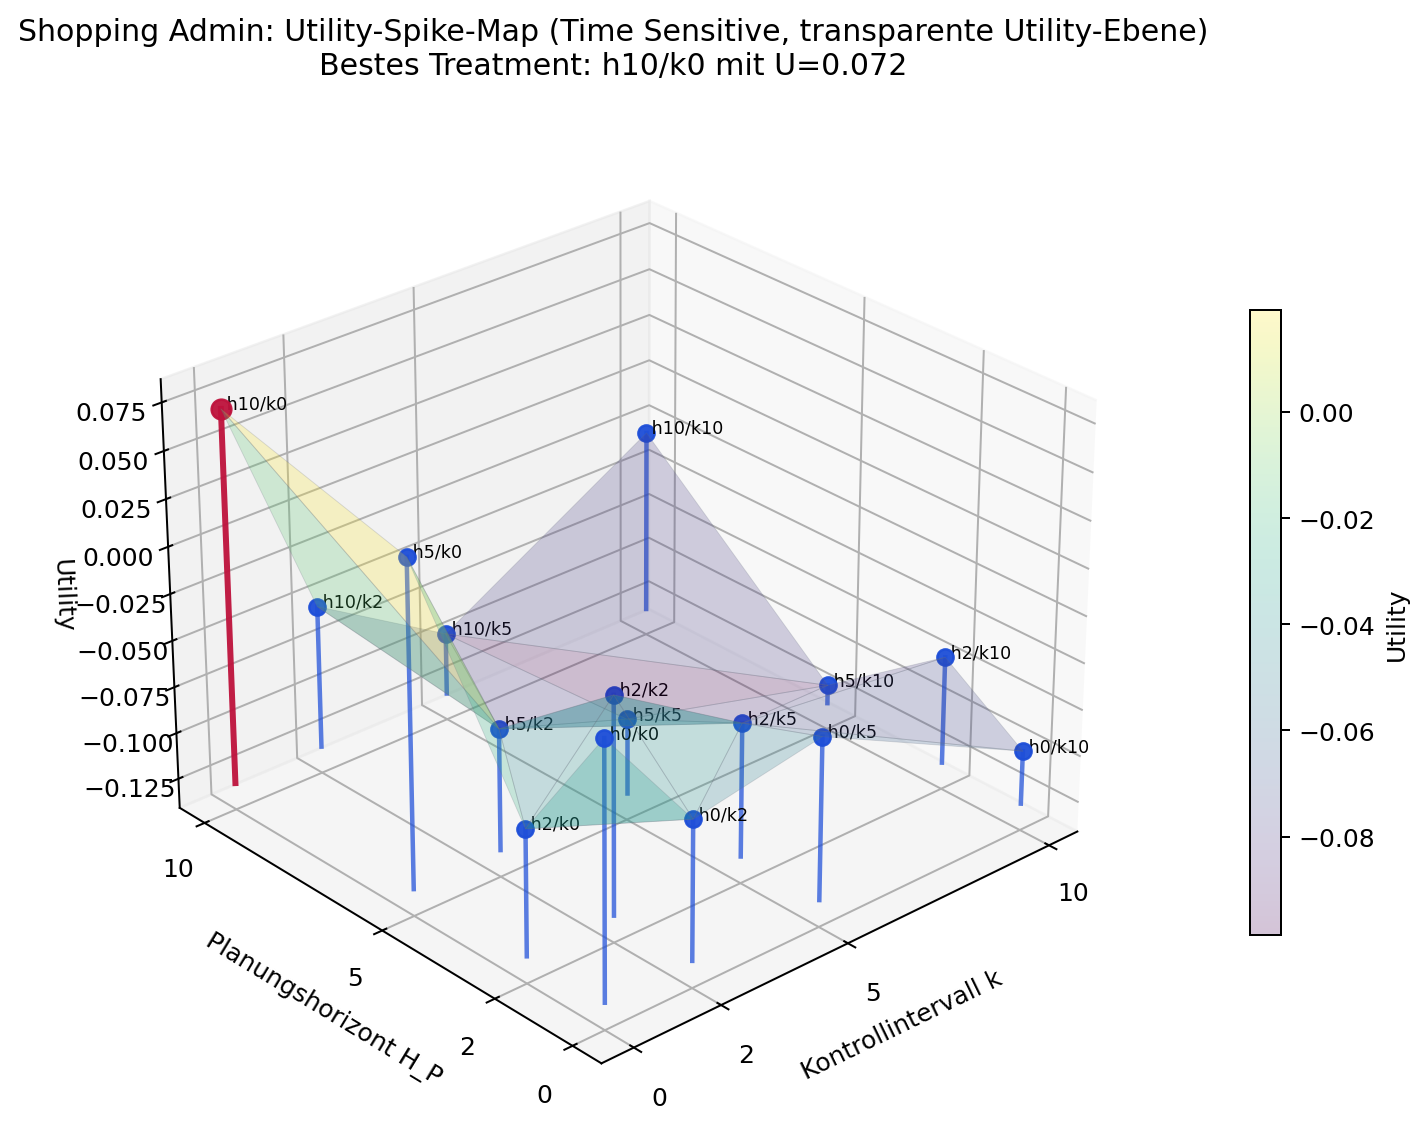
\includegraphics[width=\textwidth]
    {figures/fig_08_spike_transparent_shopping_admin_time_sensitive.png}
    \caption{Shopping Admin: Utility-Spike-Map mit transparenter Utility-Ebene für das Gewichtungsprofil Time Sensitive}
    \label{fig:app-spike-transparent-shopping-admin-time-sensitive}
\end{figure}

\begin{figure}[htbp]
    \centering
    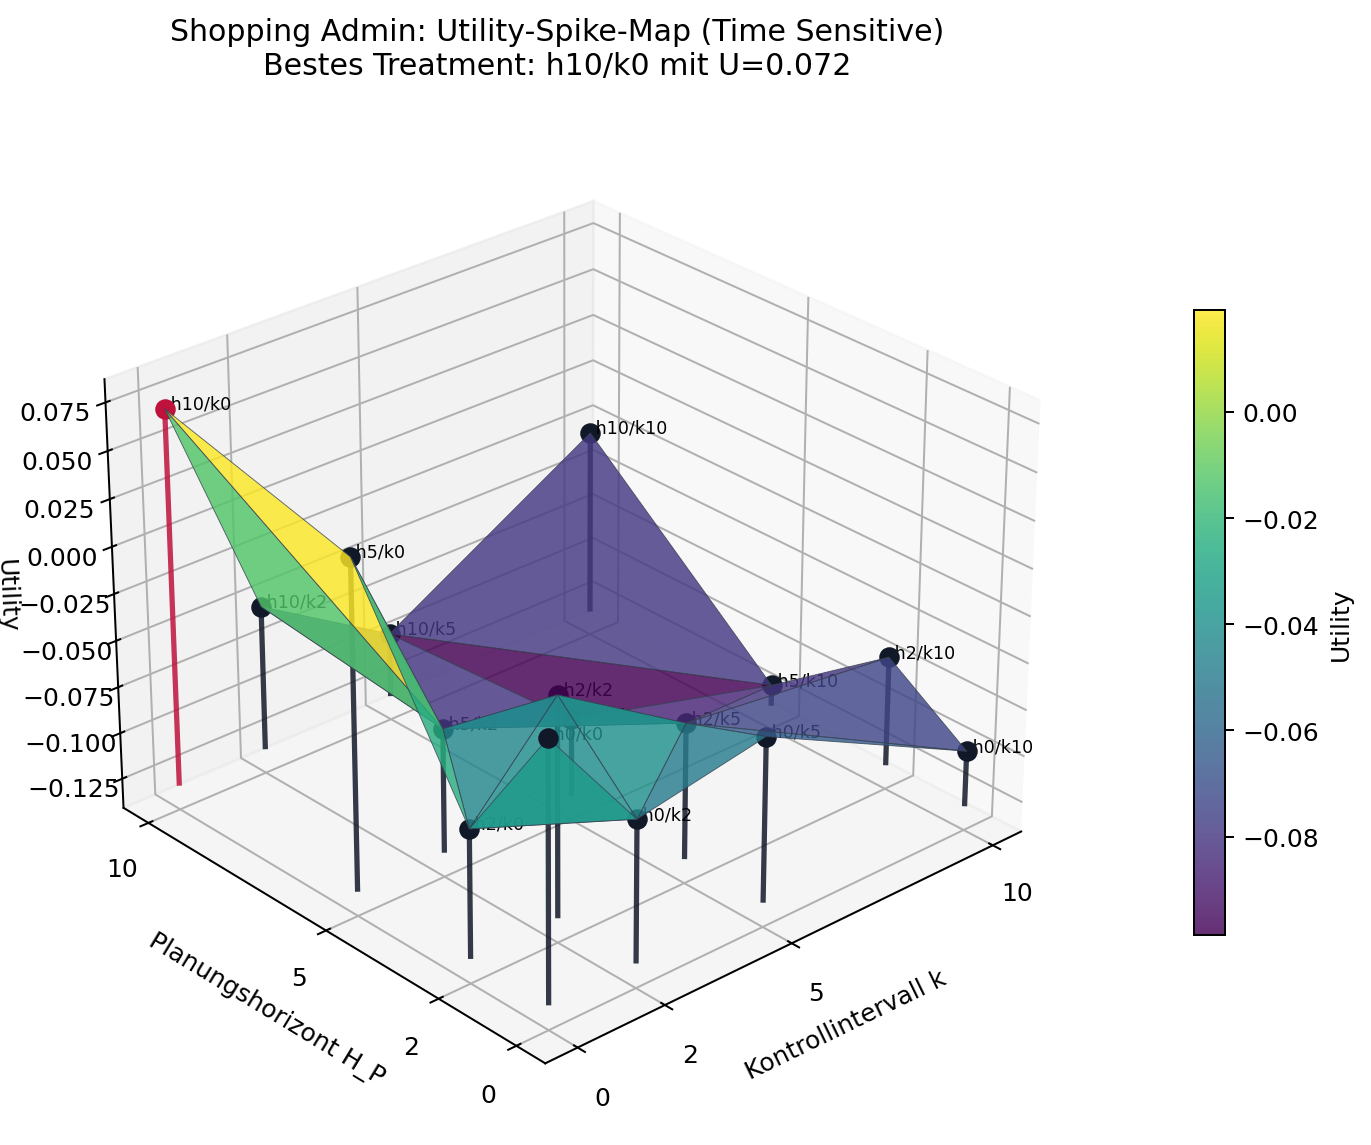
\includegraphics[width=\textwidth]
    {figures/fig_08_spike_shopping_admin_time_sensitive.png}
    \caption{Shopping Admin: Utility-Spike-Map mit kräftiger Utility-Ebene für das Gewichtungsprofil Time Sensitive}
    \label{fig:app-spike-shopping-admin-time-sensitive}
\end{figure}

\begin{figure}[htbp]
    \centering
    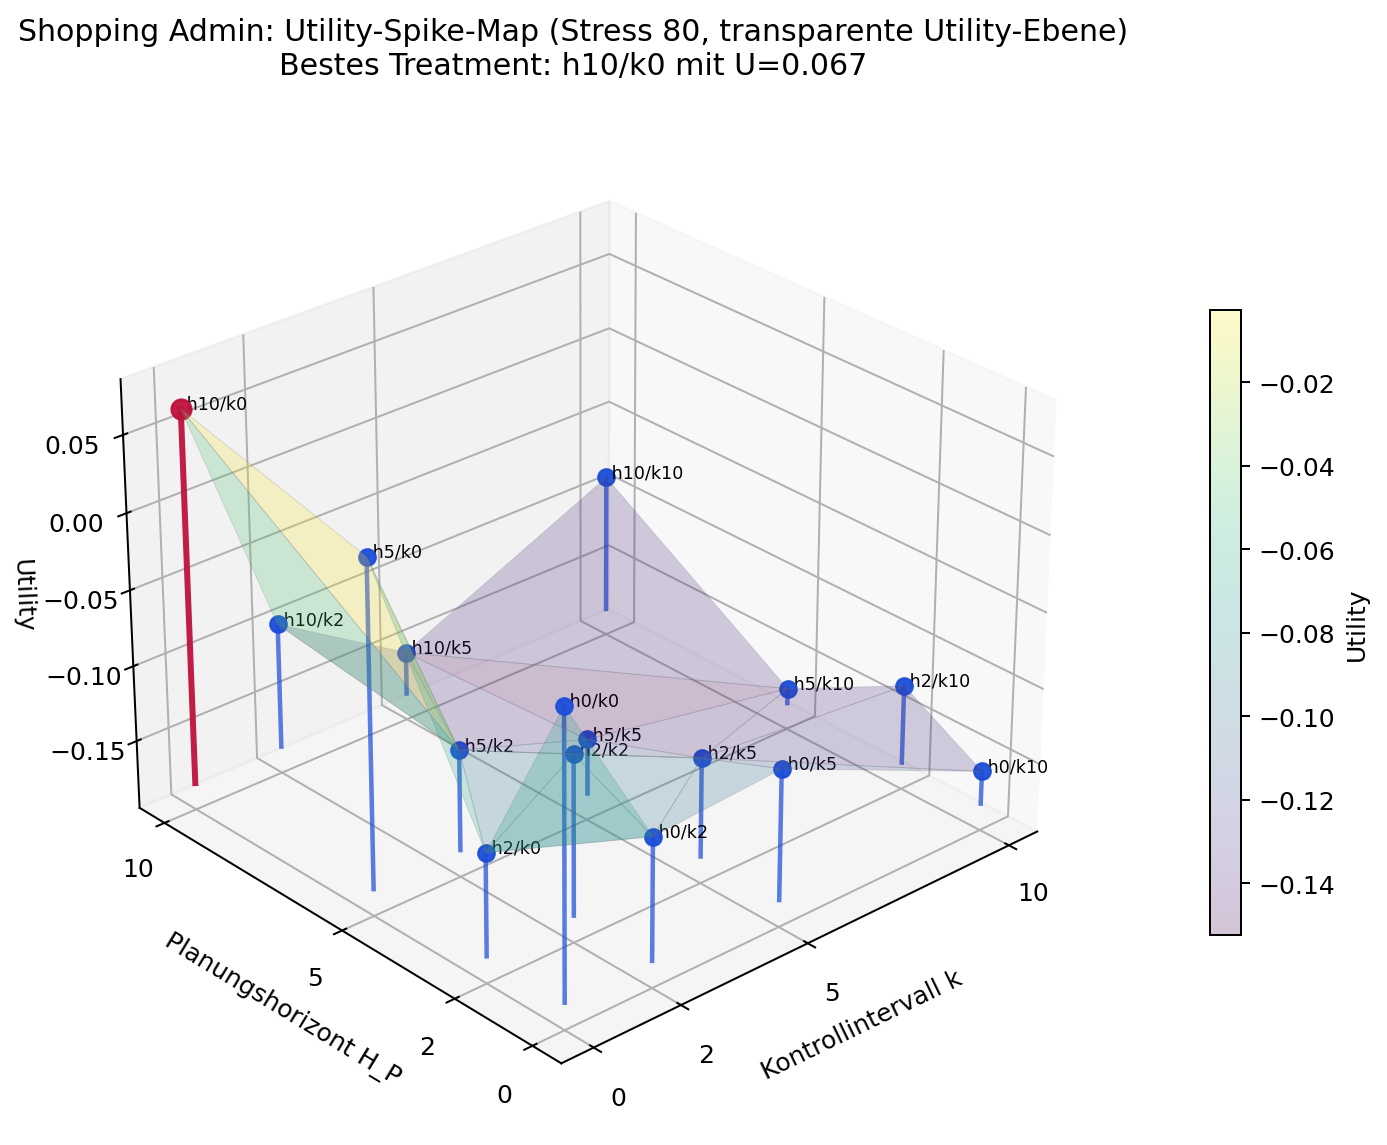
\includegraphics[width=\textwidth]
    {figures/fig_08_spike_transparent_shopping_admin_stress_80.png}
    \caption{Shopping Admin: Utility-Spike-Map mit transparenter Utility-Ebene für das Gewichtungsprofil Stress 80}
    \label{fig:app-spike-transparent-shopping-admin-stress-80}
\end{figure}

\begin{figure}[htbp]
    \centering
    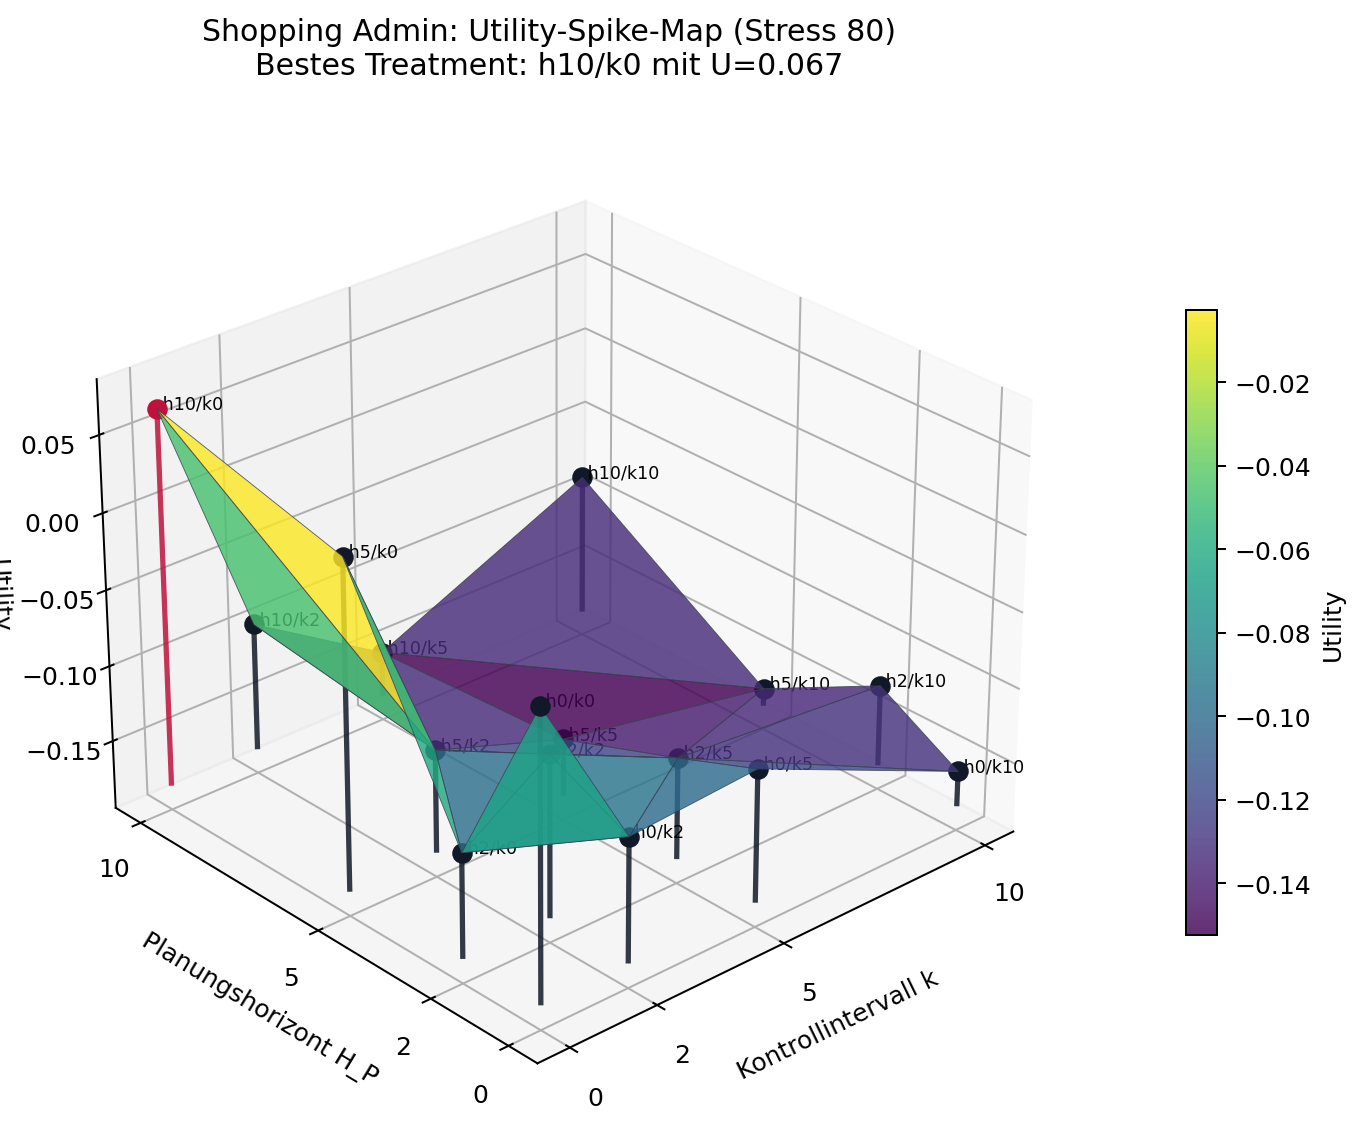
\includegraphics[width=\textwidth]
    {figures/fig_08_spike_shopping_admin_stress_80.png}
    \caption{Shopping Admin: Utility-Spike-Map mit kräftiger Utility-Ebene für das Gewichtungsprofil Stress 80}
    \label{fig:app-spike-shopping-admin-stress-80}
\end{figure}

\clearpage
\subsection{Stabilität im \(\beta/\gamma\)-Gewichtungsraum}
\label{app:beta-gamma-stabilitaet-erweitert}

Die Stabilitätskarten zeigen, welche H/k-Kombination an den jeweiligen Punkten des \(\beta/\gamma\)-Gewichtungsrasters die höchste Utility erreicht. Die anschließende Utility-Karte stellt für jeden Scope die Utility der dort stabilsten H/k-Kombination dar.

\begin{longtable}{llrrrrr}
\caption{Stabilität der H/k-Kombinationen im \(\beta/\gamma\)-Gewichtungsraum nach Scope} \label{tab:weight-space-stability-by-scope} \\
\toprule
scope & hk & weight\_points & win\_share\_pct & mean\_winner\_utility & min\_winner\_utility & max\_winner\_utility \\
\midrule
\endfirsthead
\caption[]{Stabilität der H/k-Kombinationen im \(\beta/\gamma\)-Gewichtungsraum nach Scope} \\
\toprule
scope & hk & weight\_points & win\_share\_pct & mean\_winner\_utility & min\_winner\_utility & max\_winner\_utility \\
\midrule
\endhead
\midrule
\multicolumn{7}{r}{Continued on next page} \\
\midrule
\endfoot
\bottomrule
\endlastfoot
GitLab & h5/k0 & 231 & 65,8 & 0,0958 & 0,0819 & 0,1126 \\
GitLab & h5/k5 & 119 & 33,9 & 0,1728 & 0,1191 & 0,2693 \\
GitLab & h5/k2 & 1 & 0,3 & 0,2807 & 0,2807 & 0,2807 \\
Global & h5/k5 & 136 & 38,7 & 0,1899 & 0,1210 & 0,3143 \\
Global & h10/k0 & 126 & 35,9 & 0,0675 & 0,0653 & 0,0704 \\
Global & h0/k5 & 89 & 25,4 & 0,0951 & 0,0702 & 0,1233 \\
Reddit & h5/k5 & 351 & 100,0 & 0,4708 & 0,3264 & 0,6905 \\
Shopping & h0/k2 & 264 & 75,2 & 0,0988 & 0,0544 & 0,1615 \\
Shopping & h0/k0 & 44 & 12,5 & 0,0539 & 0,0536 & 0,0543 \\
Shopping & h5/k5 & 43 & 12,3 & 0,1922 & 0,1542 & 0,2500 \\
Shopping Admin & h10/k0 & 260 & 74,1 & 0,0723 & 0,0665 & 0,0791 \\
Shopping Admin & h2/k2 & 91 & 25,9 & 0,1375 & 0,0880 & 0,2364 \\
\end{longtable}


\begin{figure}[htbp]
    \centering
    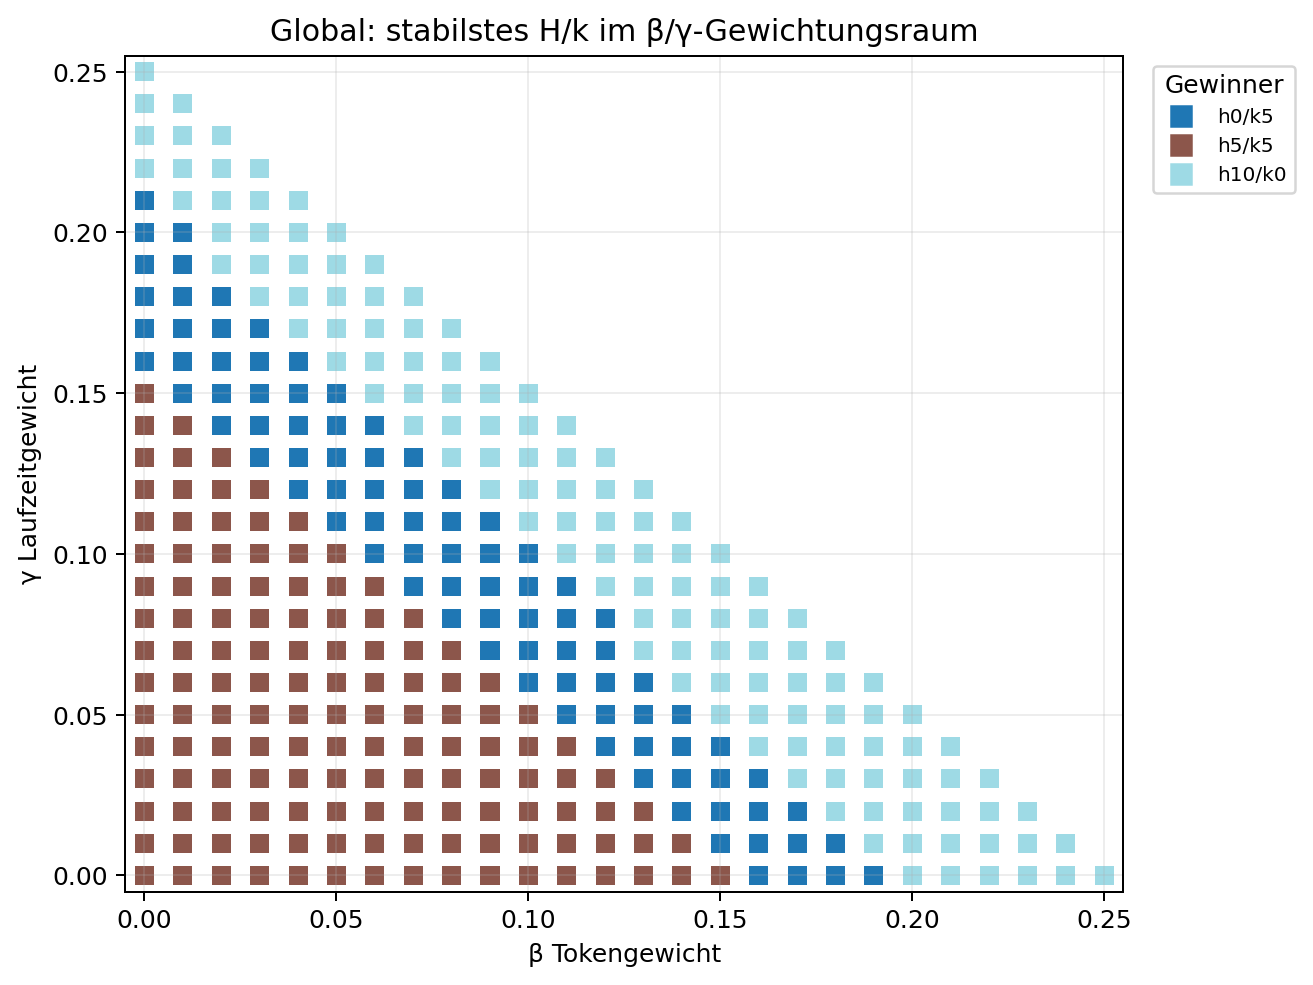
\includegraphics[width=.92\textwidth]
    {figures/fig_09_beta_gamma_winner_global.png}
    \caption{Global: stabilste H/k-Kombination im \(\beta/\gamma\)-Gewichtungsraum}
    \label{fig:app-beta-gamma-winner-global}
\end{figure}

\begin{figure}[htbp]
    \centering
    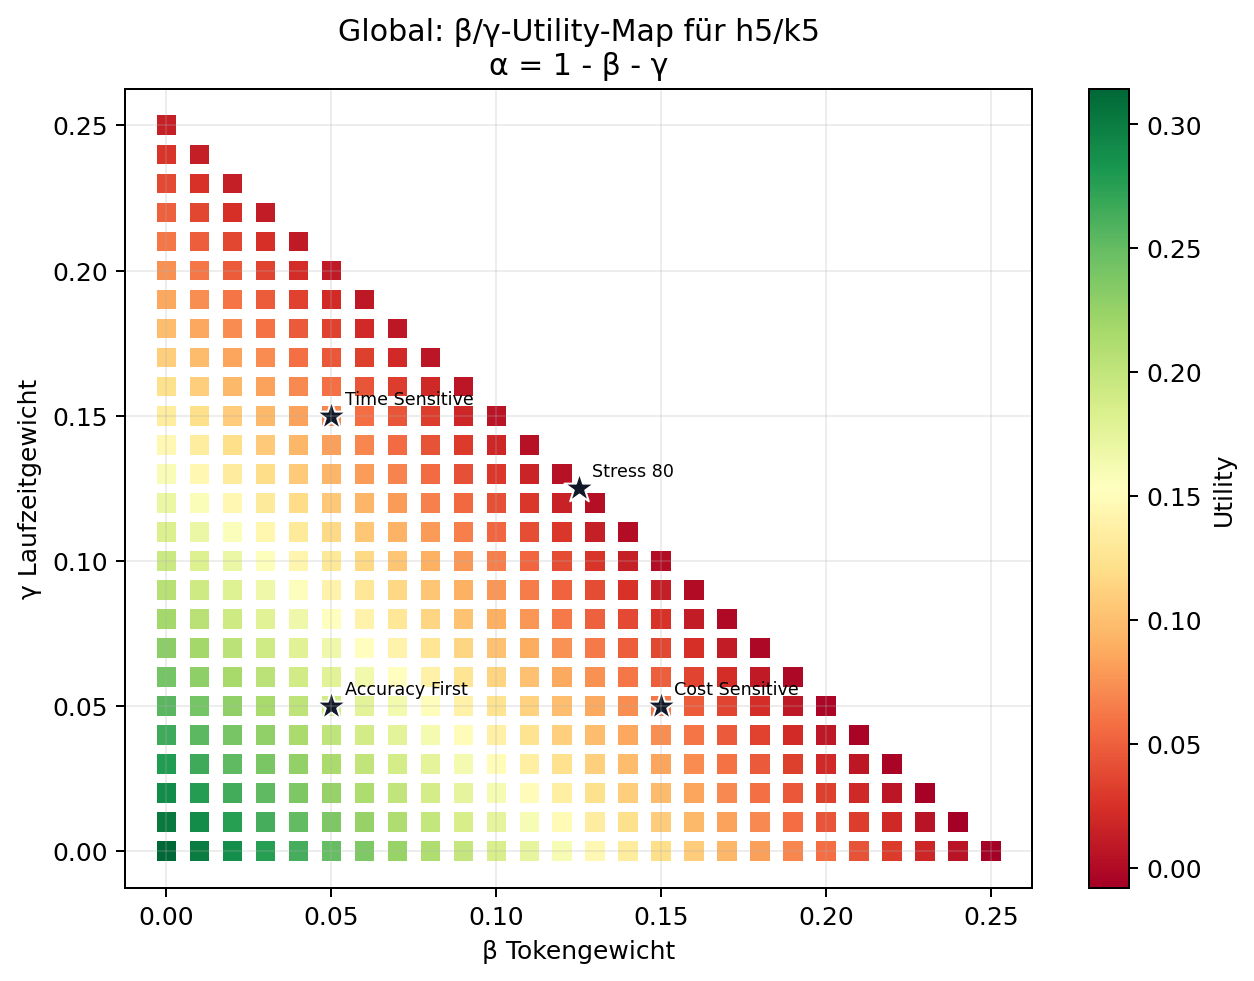
\includegraphics[width=.92\textwidth]
    {figures/fig_09_beta_gamma_utility_global_h5k5.png}
    \caption{Global: \(\beta/\gamma\)-Utility-Map für die stabilste Kombination h5/k5}
    \label{fig:app-beta-gamma-utility-global}
\end{figure}

\begin{figure}[htbp]
    \centering
    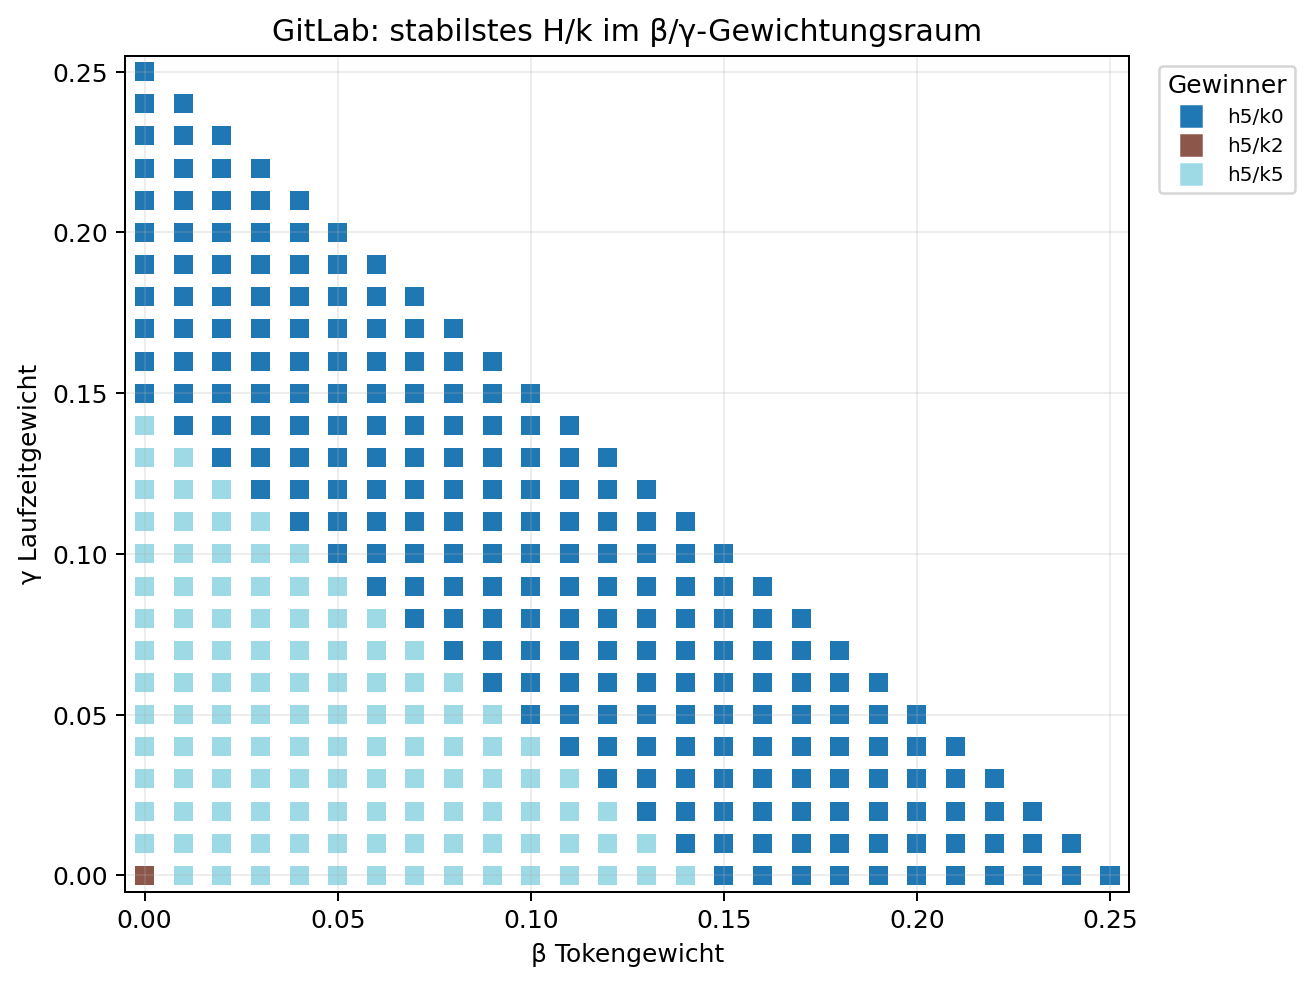
\includegraphics[width=.92\textwidth]
    {figures/fig_09_beta_gamma_winner_gitlab.png}
    \caption{GitLab: stabilste H/k-Kombination im \(\beta/\gamma\)-Gewichtungsraum}
    \label{fig:app-beta-gamma-winner-gitlab}
\end{figure}

\begin{figure}[htbp]
    \centering
    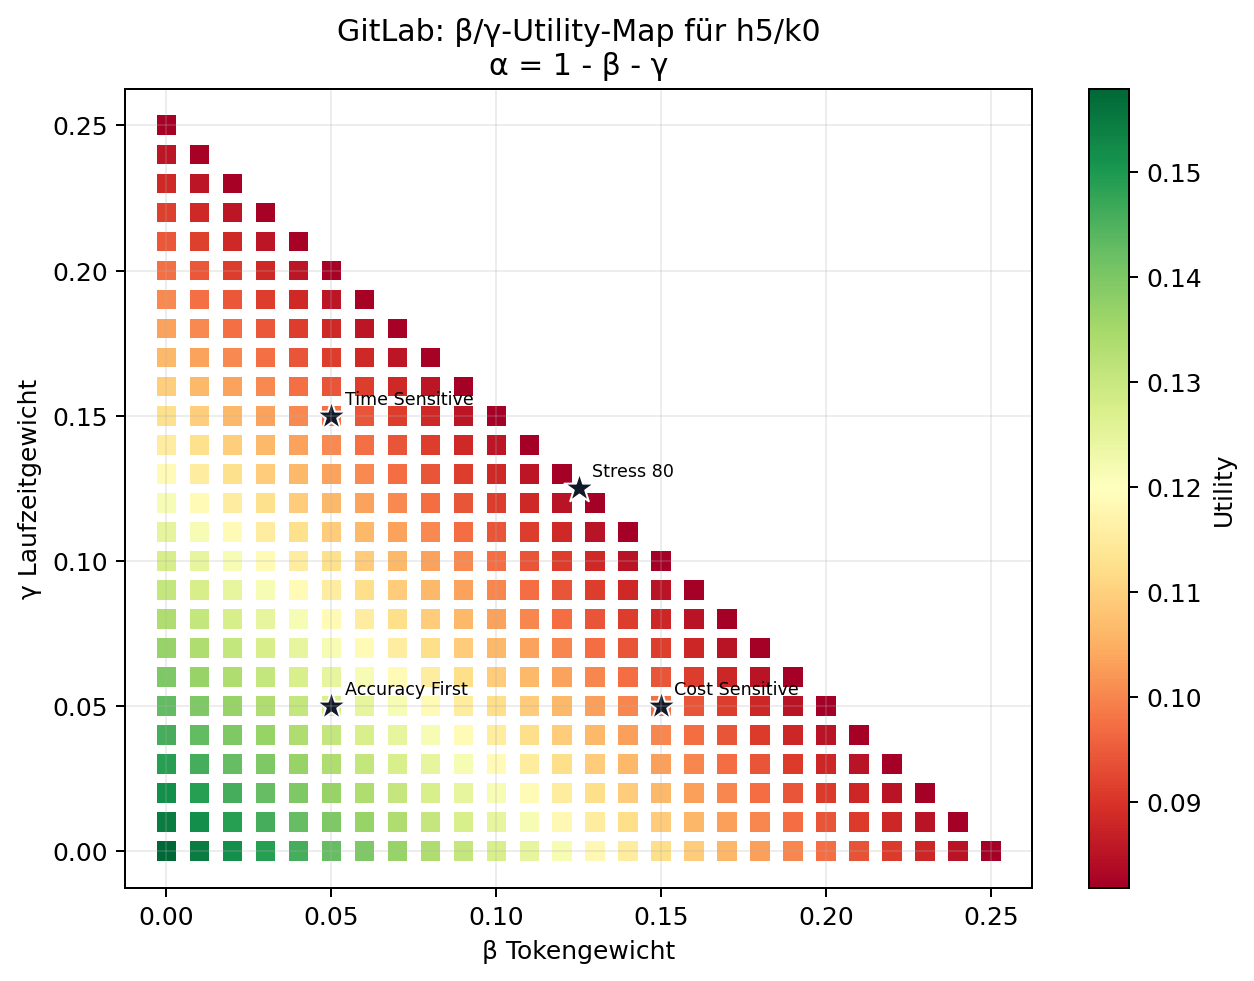
\includegraphics[width=.92\textwidth]
    {figures/fig_09_beta_gamma_utility_gitlab_h5k0.png}
    \caption{GitLab: \(\beta/\gamma\)-Utility-Map für die stabilste Kombination h5/k0}
    \label{fig:app-beta-gamma-utility-gitlab}
\end{figure}

\begin{figure}[htbp]
    \centering
    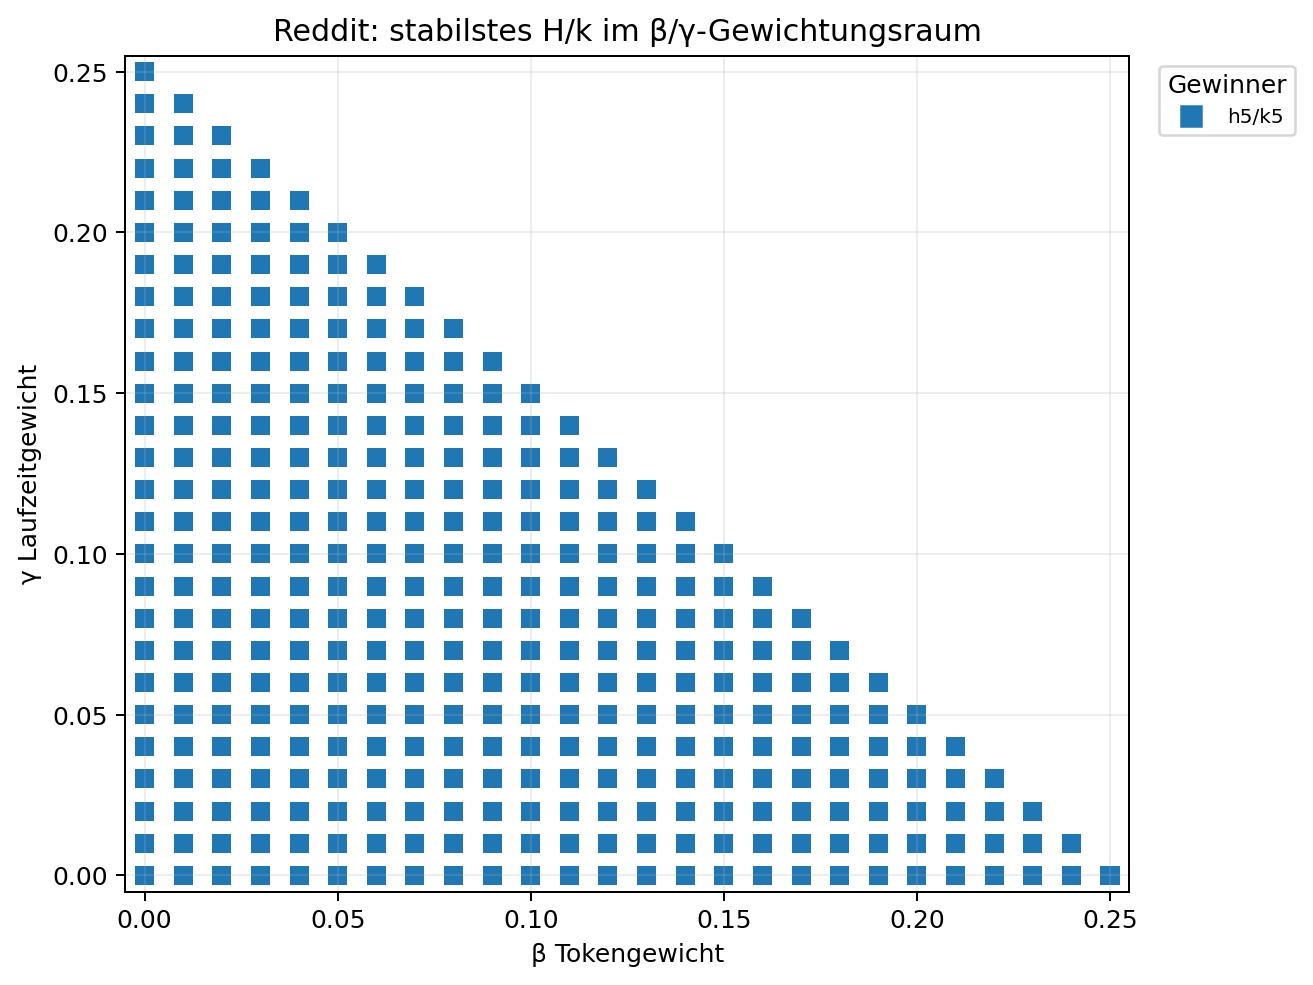
\includegraphics[width=.92\textwidth]
    {figures/fig_09_beta_gamma_winner_reddit.png}
    \caption{Reddit: stabilste H/k-Kombination im \(\beta/\gamma\)-Gewichtungsraum}
    \label{fig:app-beta-gamma-winner-reddit}
\end{figure}

\begin{figure}[htbp]
    \centering
    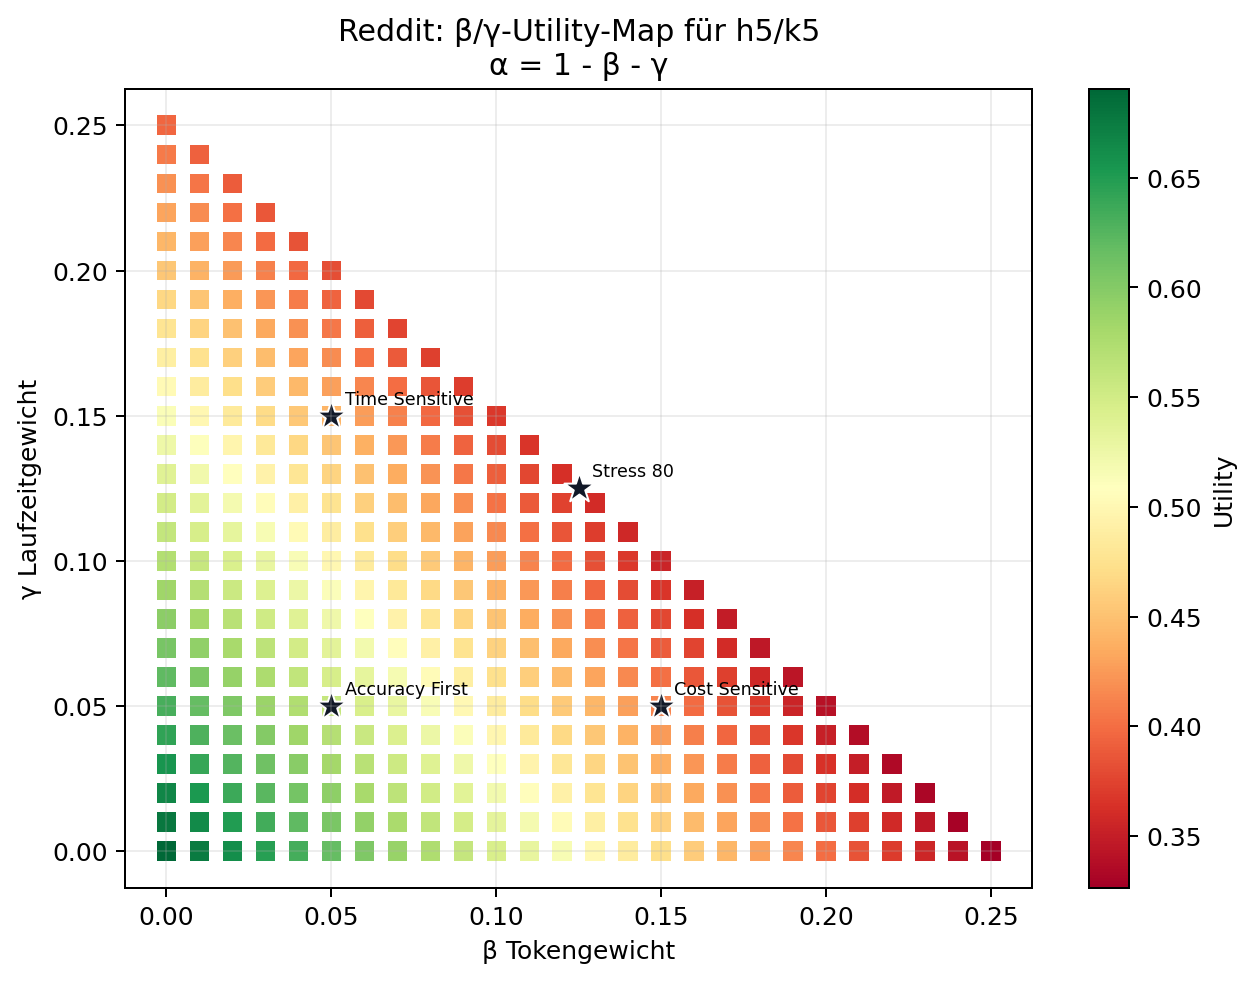
\includegraphics[width=.92\textwidth]
    {figures/fig_09_beta_gamma_utility_reddit_h5k5.png}
    \caption{Reddit: \(\beta/\gamma\)-Utility-Map für die stabilste Kombination h5/k5}
    \label{fig:app-beta-gamma-utility-reddit}
\end{figure}

\begin{figure}[htbp]
    \centering
    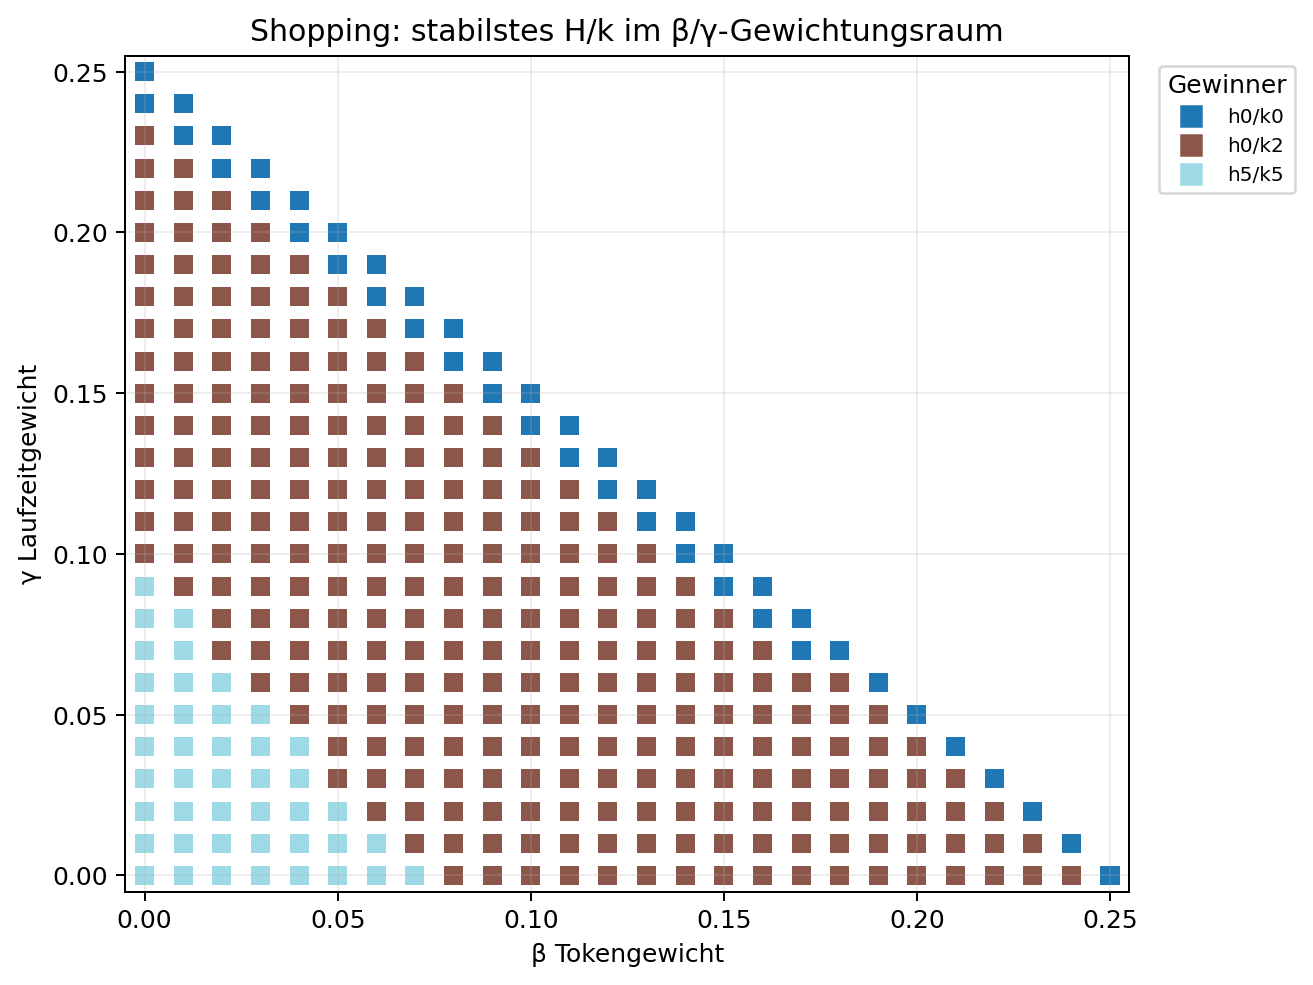
\includegraphics[width=.92\textwidth]
    {figures/fig_09_beta_gamma_winner_shopping.png}
    \caption{Shopping: stabilste H/k-Kombination im \(\beta/\gamma\)-Gewichtungsraum}
    \label{fig:app-beta-gamma-winner-shopping}
\end{figure}

\begin{figure}[htbp]
    \centering
    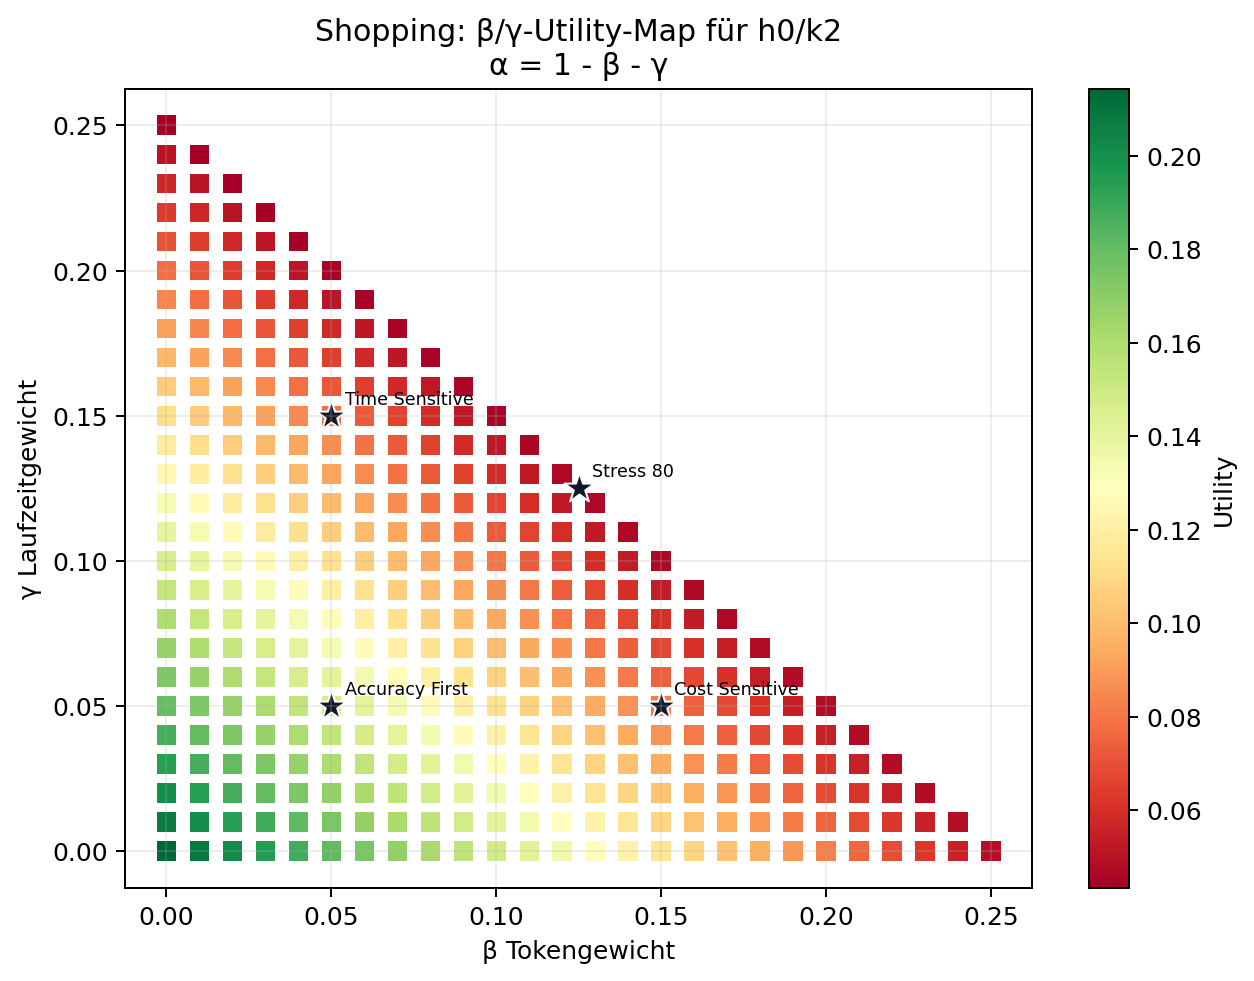
\includegraphics[width=.92\textwidth]
    {figures/fig_09_beta_gamma_utility_shopping_h0k2.png}
    \caption{Shopping: \(\beta/\gamma\)-Utility-Map für die stabilste Kombination h0/k2}
    \label{fig:app-beta-gamma-utility-shopping}
\end{figure}

\begin{figure}[htbp]
    \centering
    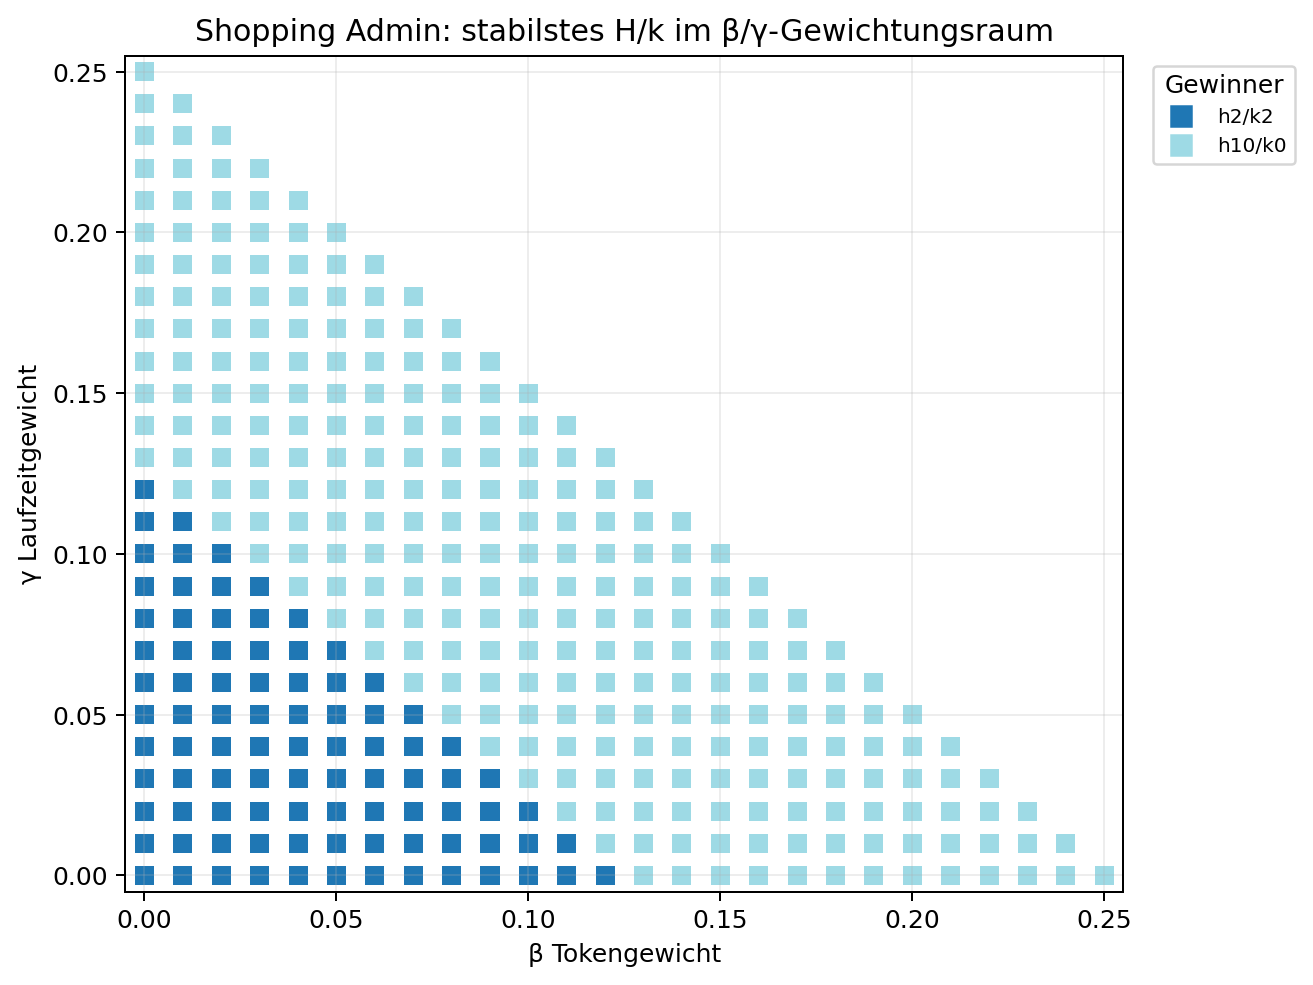
\includegraphics[width=.92\textwidth]
    {figures/fig_09_beta_gamma_winner_shopping_admin.png}
    \caption{Shopping Admin: stabilste H/k-Kombination im \(\beta/\gamma\)-Gewichtungsraum}
    \label{fig:app-beta-gamma-winner-shopping-admin}
\end{figure}

\begin{figure}[htbp]
    \centering
    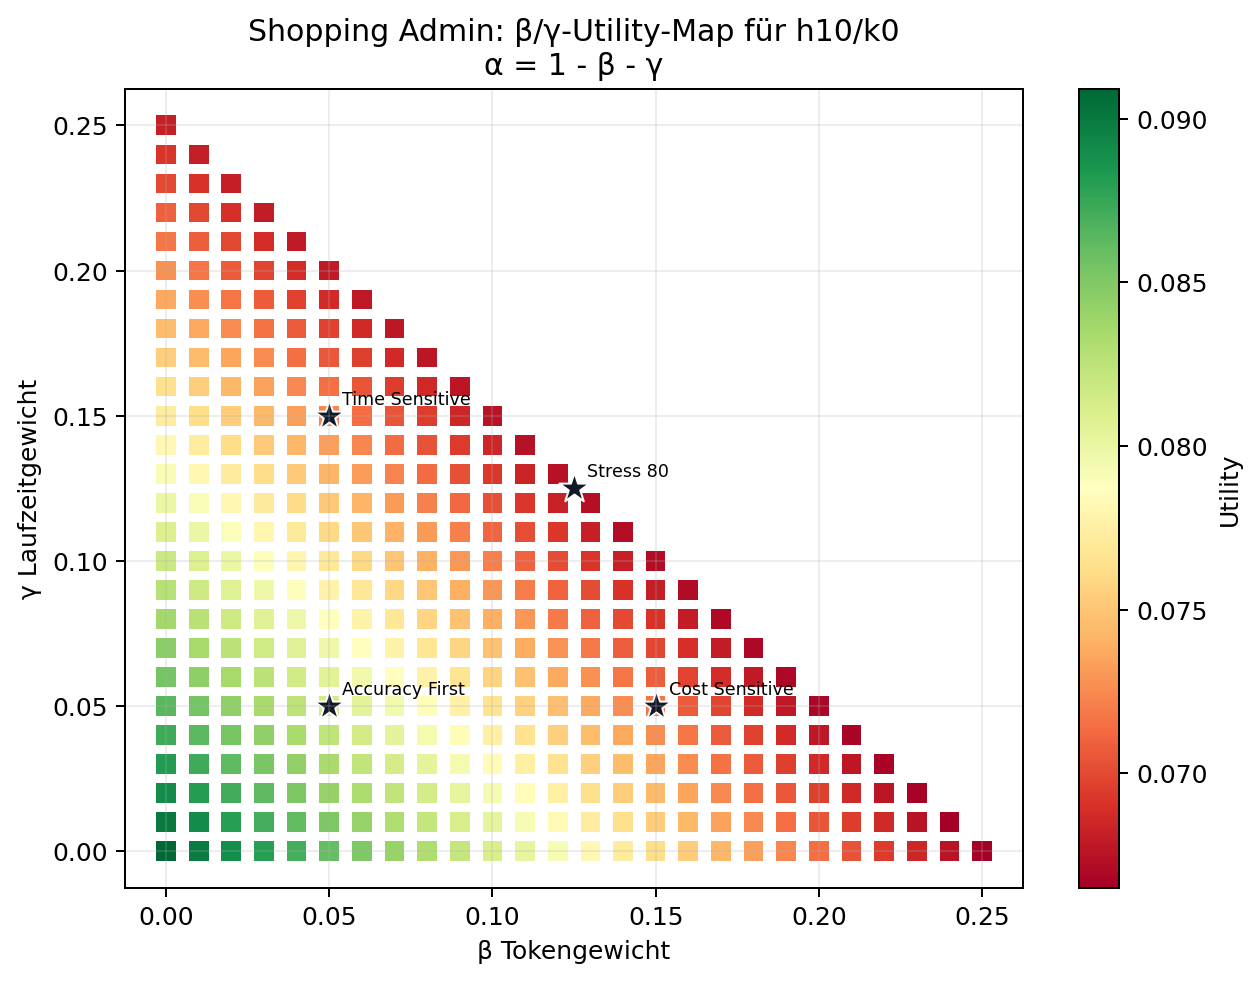
\includegraphics[width=.92\textwidth]
    {figures/fig_09_beta_gamma_utility_shopping_admin_h10k0.png}
    \caption{Shopping Admin: \(\beta/\gamma\)-Utility-Map für die stabilste Kombination h10/k0}
    \label{fig:app-beta-gamma-utility-shopping-admin}
\end{figure}

\clearpage
\subsection{Freier \(\alpha/\beta/\gamma\)-Gewichtungsraum für k=0-Baselines}
\label{app:freier-gewichtungsraum-k0}

Diese Sensitivitätsanalyse löst die success-dominante Nebenbedingung der Hauptanalyse und betrachtet den gesamten Simplex mit \(\alpha + \beta + \gamma\) = 1. Sie dient nur als Robustheitskontrolle und ersetzt nicht die im Haupttext definierte Utility-Auswertung.

\begin{longtable}{lllllrlrrlrrlrr}
\caption{Freier Gewichtungsraum: Optimum, Baselines und Utility-Spannweite für ausgewählte k=0-Treatments} \label{tab:free-weight-comparison} \\
\toprule
hk & success\_rate\_pct & avg\_tokens\_k & avg\_runtime\_s & Optimum Gewichte & U Optimum & Success-only Gewichte & U Success-only & Delta Optimum vs Success-only & Gleichgewichtet nahe & U Gleichgewichtet & Delta Optimum vs Gleichgewichtet & Minimum Gewichte & U Minimum & Utility-Spannweite \\
\midrule
\endfirsthead
\caption[]{Freier Gewichtungsraum: Optimum, Baselines und Utility-Spannweite für ausgewählte k=0-Treatments} \\
\toprule
hk & success\_rate\_pct & avg\_tokens\_k & avg\_runtime\_s & Optimum Gewichte & U Optimum & Success-only Gewichte & U Success-only & Delta Optimum vs Success-only & Gleichgewichtet nahe & U Gleichgewichtet & Delta Optimum vs Gleichgewichtet & Minimum Gewichte & U Minimum & Utility-Spannweite \\
\midrule
\endhead
\midrule
\multicolumn{15}{r}{Continued on next page} \\
\midrule
\endfoot
\bottomrule
\endlastfoot
h0/k0 & 4,3\% & 113,1k & 60,2s & \(\alpha\)=1.00, \(\beta\)=0.00, \(\gamma\)=0.00 & 0,0429 & \(\alpha\)=1.00, \(\beta\)=0.00, \(\gamma\)=0.00 & 0,0429 & +0,0000 & \(\alpha\)=0.34, \(\beta\)=0.32, \(\gamma\)=0.34 & 0,0146 & +0,0283 & \(\alpha\)=0.00, \(\beta\)=0.00, \(\gamma\)=1.00 & 0,0000 & 0,0429 \\
h5/k0 & 9,5\% & 215,4k & 85,2s & \(\alpha\)=1.00, \(\beta\)=0.00, \(\gamma\)=0.00 & 0,0952 & \(\alpha\)=1.00, \(\beta\)=0.00, \(\gamma\)=0.00 & 0,0952 & +0,0000 & \(\alpha\)=0.34, \(\beta\)=0.32, \(\gamma\)=0.34 & -0,0385 & +0,1337 & \(\alpha\)=0.00, \(\beta\)=1.00, \(\gamma\)=0.00 & -0,1305 & 0,2257 \\
h10/k0 & 9,0\% & 120,8k & 63,2s & \(\alpha\)=1.00, \(\beta\)=0.00, \(\gamma\)=0.00 & 0,0905 & \(\alpha\)=1.00, \(\beta\)=0.00, \(\gamma\)=0.00 & 0,0905 & +0,0000 & \(\alpha\)=0.34, \(\beta\)=0.32, \(\gamma\)=0.34 & 0,0242 & +0,0663 & \(\alpha\)=0.00, \(\beta\)=0.00, \(\gamma\)=1.00 & -0,0100 & 0,1005 \\
\end{longtable}

\begin{longtable}{llllrrrrrrrrrrrrrrrrrrrrr}
\caption{Freier Gewichtungsraum: Rohwerte der Gewichtskoordinaten und Extrempunkte} \label{tab:free-weight-extrema-raw} \\
\toprule
hk & success\_rate\_pct & avg\_tokens\_k & avg\_runtime\_s & T\_norm & runtime\_norm & best\_alpha & best\_beta & best\_gamma & utility\_best & worst\_alpha & worst\_beta & worst\_gamma & utility\_worst & utility\_range & alpha\_only\_alpha & alpha\_only\_beta & alpha\_only\_gamma & utility\_alpha\_only & equal\_alpha & equal\_beta & equal\_gamma & utility\_equal\_like & best\_minus\_alpha\_only & best\_minus\_equal\_like \\
\midrule
\endfirsthead
\caption[]{Freier Gewichtungsraum: Rohwerte der Gewichtskoordinaten und Extrempunkte} \\
\toprule
hk & success\_rate\_pct & avg\_tokens\_k & avg\_runtime\_s & T\_norm & runtime\_norm & best\_alpha & best\_beta & best\_gamma & utility\_best & worst\_alpha & worst\_beta & worst\_gamma & utility\_worst & utility\_range & alpha\_only\_alpha & alpha\_only\_beta & alpha\_only\_gamma & utility\_alpha\_only & equal\_alpha & equal\_beta & equal\_gamma & utility\_equal\_like & best\_minus\_alpha\_only & best\_minus\_equal\_like \\
\midrule
\endhead
\midrule
\multicolumn{25}{r}{Continued on next page} \\
\midrule
\endfoot
\bottomrule
\endlastfoot
h0/k0 & 4,3\% & 113,1k & 60,2s & 0,0000 & 0,0000 & 1,00 & 0,00 & 0,00 & 0,0429 & 0,00 & 0,00 & 1,00 & 0,0000 & 0,0429 & 1,00 & 0,00 & 0,00 & 0,0429 & 0,34 & 0,32 & 0,34 & 0,0146 & 0,0000 & 0,0283 \\
h5/k0 & 9,5\% & 215,4k & 85,2s & 0,1305 & 0,0856 & 1,00 & 0,00 & 0,00 & 0,0952 & 0,00 & 1,00 & 0,00 & -0,1305 & 0,2257 & 1,00 & 0,00 & 0,00 & 0,0952 & 0,34 & 0,32 & 0,34 & -0,0385 & 0,0000 & 0,1337 \\
h10/k0 & 9,0\% & 120,8k & 63,2s & 0,0098 & 0,0100 & 1,00 & 0,00 & 0,00 & 0,0905 & 0,00 & 0,00 & 1,00 & -0,0100 & 0,1005 & 1,00 & 0,00 & 0,00 & 0,0905 & 0,34 & 0,32 & 0,34 & 0,0242 & 0,0000 & 0,0663 \\
\end{longtable}


\begin{figure}[htbp]
    \centering
    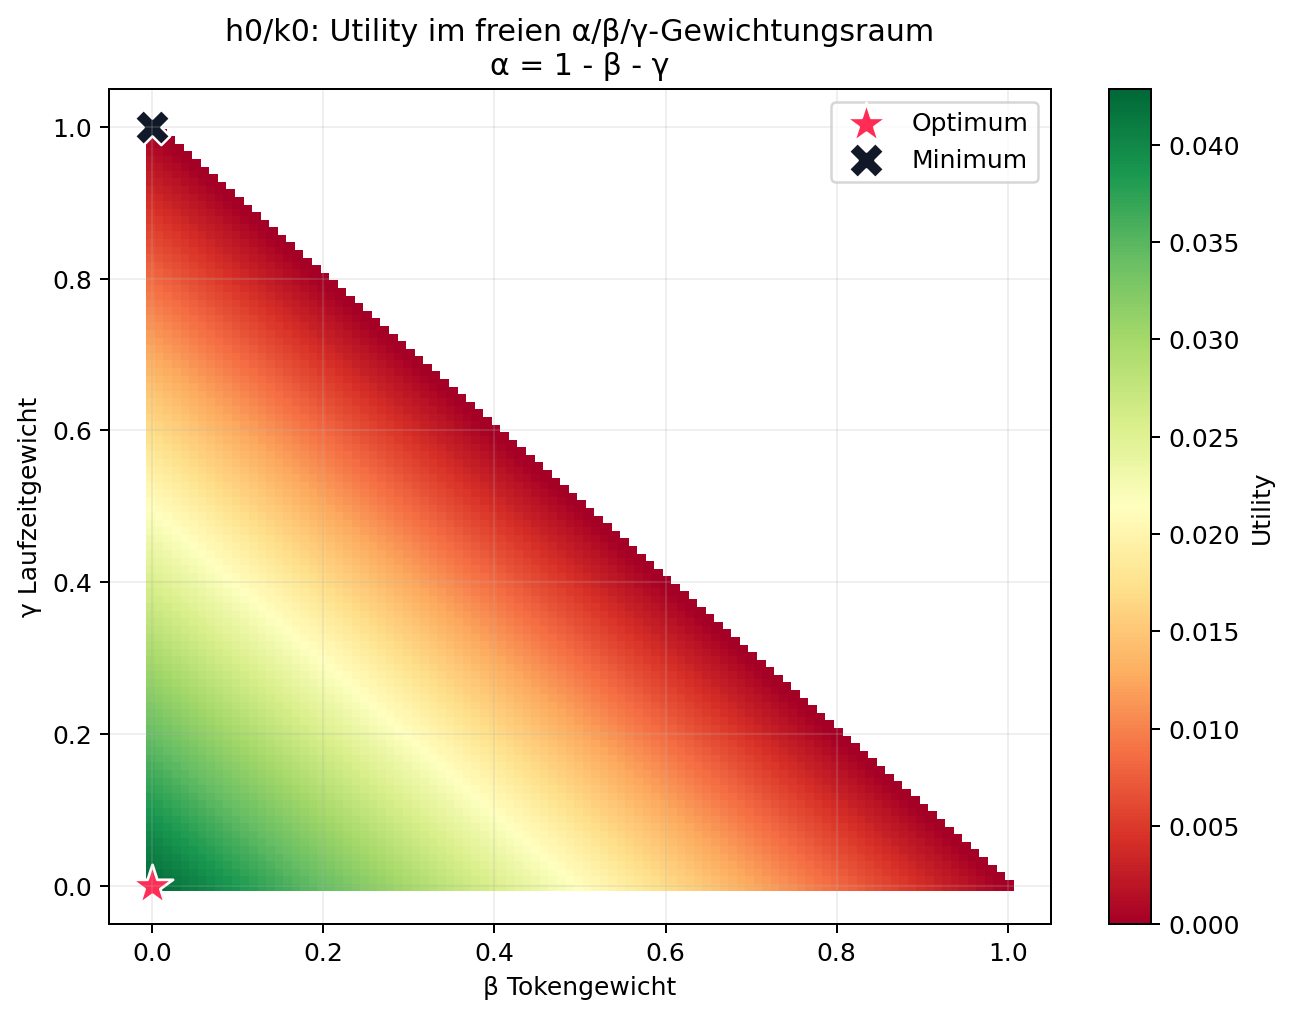
\includegraphics[width=.92\textwidth]
    {figures/fig_10_free_weight_h0k0.png}
    \caption{h0/k0: Utility im freien \(\alpha/\beta/\gamma\)-Gewichtungsraum}
    \label{fig:app-free-weight-h0k0}
\end{figure}

\begin{figure}[htbp]
    \centering
    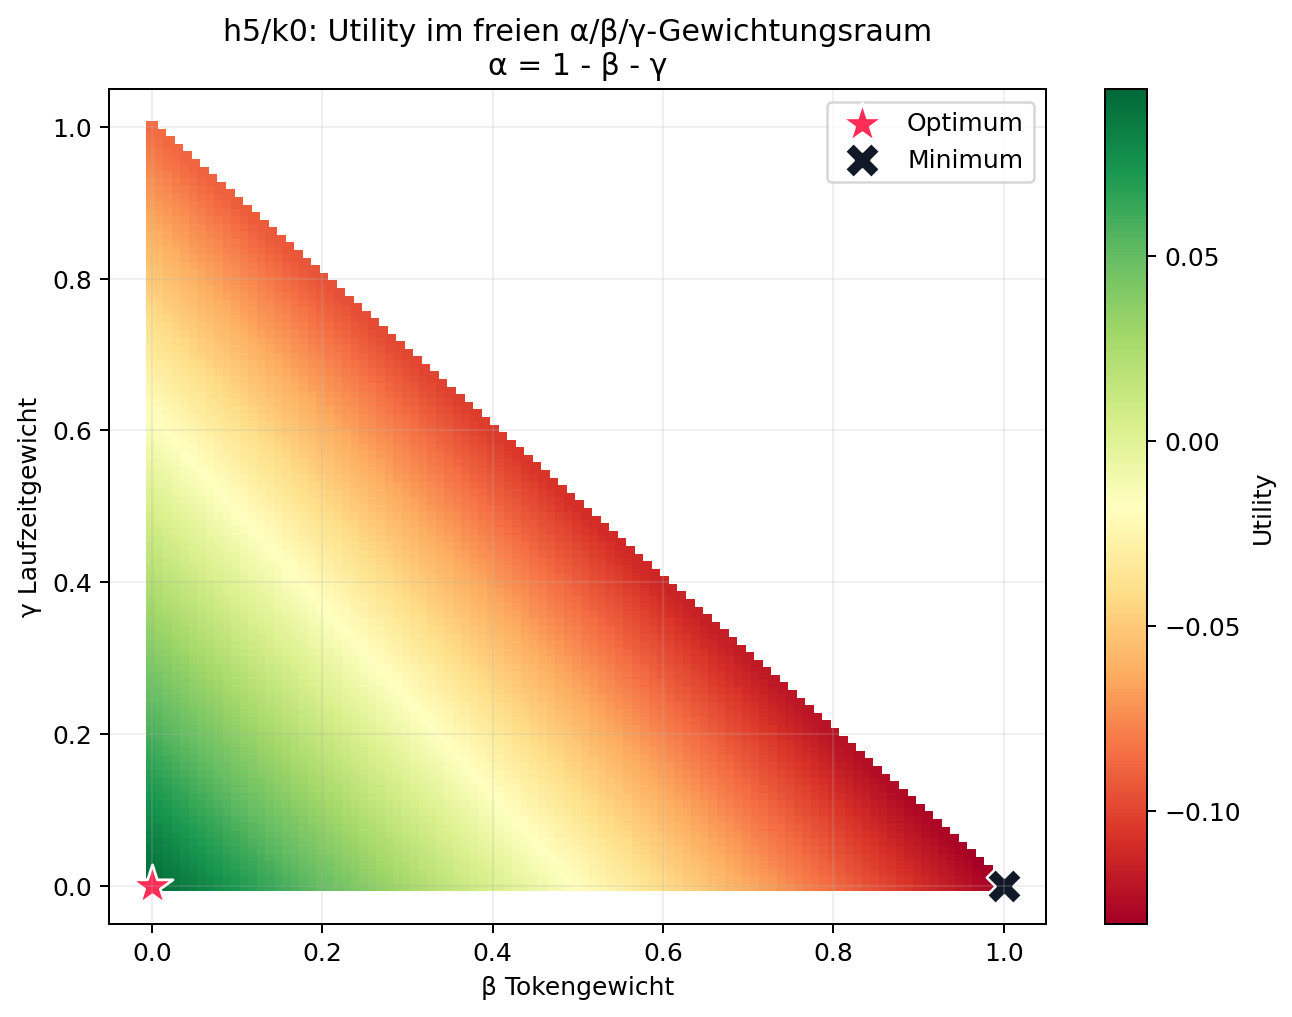
\includegraphics[width=.92\textwidth]
    {figures/fig_10_free_weight_h5k0.png}
    \caption{h5/k0: Utility im freien \(\alpha/\beta/\gamma\)-Gewichtungsraum}
    \label{fig:app-free-weight-h5k0}
\end{figure}

\begin{figure}[htbp]
    \centering
    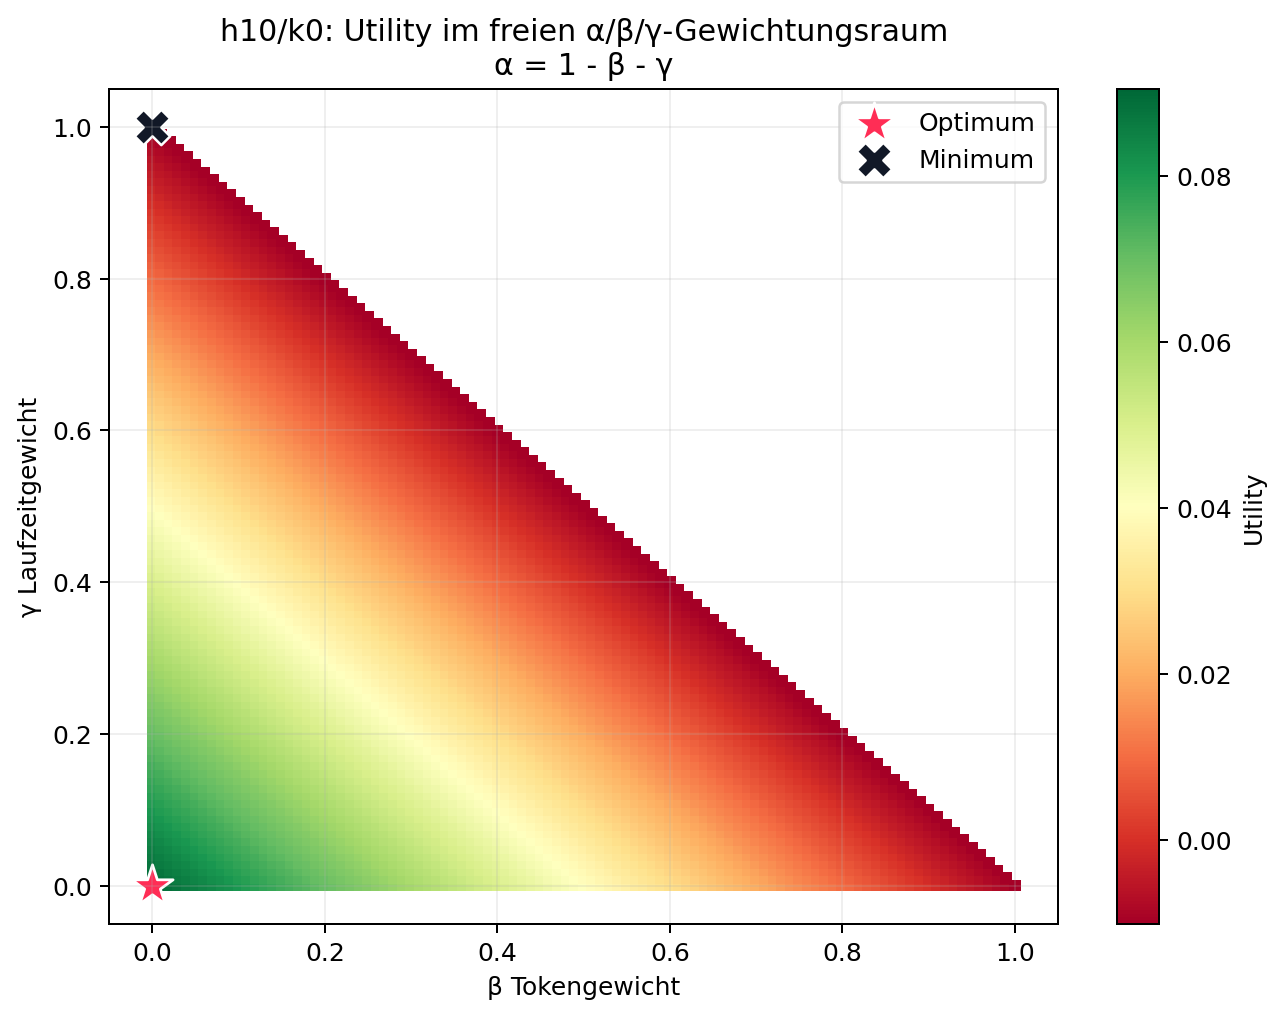
\includegraphics[width=.92\textwidth]
    {figures/fig_10_free_weight_h10k0.png}
    \caption{h10/k0: Utility im freien \(\alpha/\beta/\gamma\)-Gewichtungsraum}
    \label{fig:app-free-weight-h10k0}
\end{figure}
